\documentclass[pra,twocolumn,superscriptaddress,nofootinbib,floatfix]{revtex4-2}
\usepackage[T1]{fontenc}
\usepackage[utf8]{inputenc}
\usepackage{amsmath,amssymb,amsfonts,amsthm,bm}
\usepackage{physics}
\usepackage{graphicx}
\usepackage{booktabs}
\usepackage{array}
\newcolumntype{L}[1]{>{\raggedright\arraybackslash}p{#1}}
\usepackage{xcolor}
\usepackage[colorlinks=true,linkcolor=blue,citecolor=blue,urlcolor=blue]{hyperref}

\newtheorem{theorem}{Theorem}
\newtheorem{proposition}{Proposition}
\newtheorem{definition}{Definition}
\theoremstyle{remark}
\newtheorem*{remark}{Remark}

\newcommand{\dpr}{d_{\rm pr}}

\begin{document}

\title{Native nonlinear interactions versus programmable emulation in hybrid oscillator--qubit simulation}

\author{Elin Ranjan Das}
\author{Muqing Zheng}
\author{Tim Stavenger}
\author{Yuan Liu}
\affiliation{Pacific Northwest National Laboratory, Richland, Washington 99354, USA}

\date{\today}

\begin{abstract}
Superconducting oscillator--qubit processors contain nonlinear interactions, such as the Josephson cosine and the Kerr effect, that also appear in classical nonlinear equations of motion. We ask when such native interactions can supply the nonlinear part of a target Hamiltonian dynamics directly, and how much programmable control native evolution saves compared with emulating the same evolution with programmable gates. The comparison uses an ideal gate model, in which native evolution for a chosen time is one operation that can be switched on and off between gates. We organize the native interactions into dictionaries of Hamiltonian terms, bound the error of omitting a correction by a phase-insensitive residual bound along the native trajectory, and read classical trajectories from the quantum first moments only inside a mean-field window, which on a sine-Gordon Josephson lattice depends on the initial phase spread as well as on the Josephson energy. For a Duffing oscillator built from a Kerr mode, the omitted number-changing terms cannot be restored by any number-diagonal control, and a compiled correction keeps the state error below $\sqrt{10^{-3}}$ on ten development inputs and twelve held-out coherent states. Each native Kerr wait can, however, be replaced without loss of accuracy by one number-selective phase gate with analytic phases, so the native interaction saves only 11 of 131 such gates. For a two-site double sine-Gordon lattice, native evolution with a trigonometric correction meets the same criterion with 64 programmable primitives, against 209 for the best programmable circuit tested, which implements the quadratic terms as one Gaussian block. Native evolution leaves only the correction to be compiled and split from the rest of the Hamiltonian, and the saving stays between 2.6 and 4.6 over three second-harmonic strengths, a tenfold range of infidelity thresholds, and a three-site lattice.
\end{abstract}

\maketitle

\section{Introduction}
\label{sec:intro}

\begin{table*}[t]
\caption{Benchmarks of this work. The class is defined in Sec.~\ref{subsec:native-match}, and the counts refer to circuits of Sec.~\ref{sec:benchmarks} that meet its accuracy criterion in the ideal gate model, which for the double sine-Gordon lattice are the cheapest found. The lossy Kerr array of Appendix~\ref{app:lchs}, of class I--N, is analyzed without numerical simulation.}
\label{tab:classes}
\begin{ruledtabular}
\begin{tabular}{L{2.5cm}L{0.8cm}L{3.5cm}L{4.1cm}L{4.4cm}}
Benchmark & Class & Native evolution and correction & Programmable emulation of the native evolution & Result \\
\hline
Sine-Gordon lattice & I--U & Josephson lattice, no correction & not compared & first moments follow the classical field inside a mean-field window \\
Duffing oscillator & II--U & Kerr mode, number-changing quartic correction & one SNAP gate per native wait, with analytic phases & native waits save 11 of 131 SNAP gates \\
Double sine-Gordon lattice & II--U & Josephson lattice, second-harmonic correction & trigonometric gates for the cosine and a product formula & 64 against 209 programmable primitives on two sites \\
\end{tabular}
\end{ruledtabular}
\end{table*}

Nonlinear ordinary and partial differential equations govern a wide range of physical systems, including fluid dynamics, biological reaction-diffusion processes, coupled waveguide arrays \cite{Christodoulides2003Discretizing}, and nonlinear wave propagation in periodic media, where they describe phenomena such as discrete and gap solitons \cite{newell1985solitons}. General-purpose quantum algorithms for nonlinear dynamics typically begin by embedding the nonlinear problem into a larger linear system. Carleman linearization \cite{Liu_2021,doi:10.1137/24M1665799}, Koopman--von Neumann methods \cite{Joseph_2020,brunton2021modernkoopmantheorydynamical}, and multiple-copy constructions \cite{lloyd2020quantumalgorithmnonlineardifferential, tennie2024quantumcomputingnonlineardifferential} all employ variants of this strategy, with convergence guarantees under assumptions such as dissipation dominance \cite{Krovi_2023,tennie2024quantumcomputingnonlineardifferential}. These methods are broadly applicable, but the enlarged linear generator must still be represented and compiled on the target processor.
A recent oracle-free hybrid oscillator--qubit algorithm follows a density-based route \cite{chandramouli2026provableoraclefreequantumalgorithm}. It maps polynomial nonlinear ordinary differential equations to a Fokker--Planck evolution \cite{10.1098/rspa.2025.0016}, applies a warped-phase transformation to the resulting linear nonunitary generator \cite{Jin_2024_schrodingerization}, and carries the Fourier-mode parameter on a single continuous-variable mode \cite{Jin_2024_qumodization}. Its explicit decomposition into commuting families of monomial-controlled momentum displacements removes sparse-access oracles and block encodings. Related proposals use several bosonic modes coupled to qubits to solve nonlinear differential equations \cite{gan2025provablyefficientquantumalgorithms}.

The same nonlinear structures appearing in the differential equations themselves arise, in quantized form, as native interactions in hybrid superconducting oscillator--qubit processors \cite{Liu_2026}. The Josephson junction supplies a cosine potential \cite{JOSEPHSON1962251, Blais_2021}, a detuned cavity mode behaves as a Kerr oscillator \cite{Kirchmair_2013, Nigg_2012}, asymmetric Josephson elements generate three- and four-wave mixing \cite{Frattini_2017, Frattini_2018}, and coupled circuit elements form nonlinear bosonic lattices \cite{Fitzpatrick_2017, Fedorov_2021}. This correspondence between nonlinear differential-equation structure and native circuit interactions motivates a complementary approach: rather than first embedding the nonlinear dynamics into a larger linear problem and subsequently compiling the resulting generator, one may ask whether the nonlinear vector field itself can be approximated directly within the function class naturally supported by the hardware.

In this work, we ask the following question:

\emph{Given a nonlinear vector field \(\mathbf f\), what class of vector fields can a programmable Josephson circuit approximate directly, which part of the dynamics must be supplied by programmable corrections to reach error \(\epsilon\), how do the omitted and compiled parts propagate to the dynamical solution, and when does native evolution reduce the programmable cost compared with emulating the same evolution?}

A closed circuit generates Hamiltonian dynamics, so the directly accessible vector fields are Hamiltonian flows. The circuit also evolves the quantized model, whose first moments follow the classical equation only while a mean-field closure holds. The accuracy targets below therefore refer to the quantum state and to quantum observables, and the classical equation is read from the first moments only inside a mean-field window. Koopman--von Neumann embeddings avoid this restriction by evolving a classical wavefunction under the Liouville generator of the flow, with commuting position and momentum operators, and they have been studied for continuous-variable photonic processors \cite{gao2025implementingkoopmanvonneumannapproach}.

The native interaction also rarely equals the target Hamiltonian, and the remainder must either be omitted with a controlled error or be implemented with programmable controls. A native interaction then saves programmable resources only relative to a programmable emulation of the same evolution. Both routes have precedents for the models studied here. Josephson-junction arrays have been analyzed as analog simulators of the quantum sine-Gordon model, including its vertex correlations and entanglement \cite{Roy2021}, and arrays with \(0\)--\(\pi\) qubits add a second cosine harmonic \cite{RoyLukyanov2023Confinement,Roy2023Multicritical}. Selective number-dependent arbitrary phase (SNAP) gates implement any number-diagonal evolution, including Kerr evolution \cite{Krastanov_2015,Heeres_2015}, and trigonometric continuous-variable gates implement the Josephson cosine with an ancillary qubit and have been used to simulate the real-time dynamics, vertex correlations, and kink profiles of the lattice sine-Gordon model \cite{Rainaldi2026TrigonometricCV}. Digital--analog schemes combine native evolution with digital blocks \cite{ParraRodriguez2020DAQC,DigitalAnalogFermionBoson2025}, and gate-level resource estimates exist for bosonic simulation on hybrid oscillator--qubit processors \cite{Crane2024Hybrid}.

We add to them a comparison, under a common accuracy criterion, between native evolution with a compiled correction and programmable emulation of the same evolution. The cheapest programmable circuits tested implement all quadratic terms as one Gaussian block, and for every route we scan the number of steps and the block orders. In both benchmarks with a correction, the saving follows the cost of the best programmable emulation tested and not the nonlinearity of the interaction itself. The error analysis uses a residual bound along the native trajectory, which applies the Duhamel estimate of phase-agnostic residual methods \cite{Zoufal2023} with an available native Hamiltonian as the reference, and a composition bound on the exact target trajectory. For specified inputs these bounds give sufficient conditions for omitting a correction and for accepting a compiled one.

All circuit comparisons use an ideal gate model. Native evolution for a chosen time counts as one operation that can be switched on and off, so the native Hamiltonian is assumed to be off or refocused while programmable gates act, and programmable primitives are counted without noise, calibration error, or duration. The model isolates the part of the programmable cost that native evolution removes, the compilation of the native interaction and the extra product-formula steps forced by its commutators with the rest of the Hamiltonian. Switching adds a platform-dependent cost to each native wait, and residual drift affects both routes. The lattice benchmarks treat each Josephson phase as an extended coordinate (Sec.~\ref{subsec:sg-model}), and the Duffing benchmark uses a Kerr mode of either sign in a frame rotating at its carrier frequency (Sec.~\ref{subsec:df-reduction}). The switchable native block is the strongest of these assumptions for a Josephson lattice, whose native evolution cannot be paused in a fixed-capacitance array. The lattice results are therefore resource comparisons within the gate model, and Sec.~\ref{subsec:hardware} discusses what a device would have to provide.

Section~\ref{sec:framework} organizes the Josephson dictionaries, identifies the Hamiltonian flows they generate, and classifies a target by whether native evolution alone reproduces its Hermitian sector. It bounds the error of omitting a correction by a residual bound along the native trajectory, controls repeated hybrid steps by a composition bound on the exact target trajectory, and defines the emulation cost against which native evolution is measured. Section~\ref{sec:benchmarks} applies the framework to three unitary benchmarks with different roles, summarized in Table~\ref{tab:classes}. The sine-Gordon lattice needs no correction, and we use it to map the window in which the first moments follow the classical field. The Duffing oscillator needs a number-changing correction, and its native Kerr interaction is emulated exactly by SNAP gates, so native evolution saves few programmable gates. The double sine-Gordon lattice needs a cosine correction to a native Josephson lattice, whose emulation requires a product formula, and native evolution saves about a factor of three in programmable primitives relative to the best programmable circuit tested. Figure~\ref{fig:overview} summarizes the implementations and the two readings of the output. Section~\ref{sec:discussion} discusses what a native interaction is worth, physical duration, the hardware model, and the limits of these finite-model results.

\section{Framework}
\label{sec:framework}

\begin{figure*}[t]
\centering
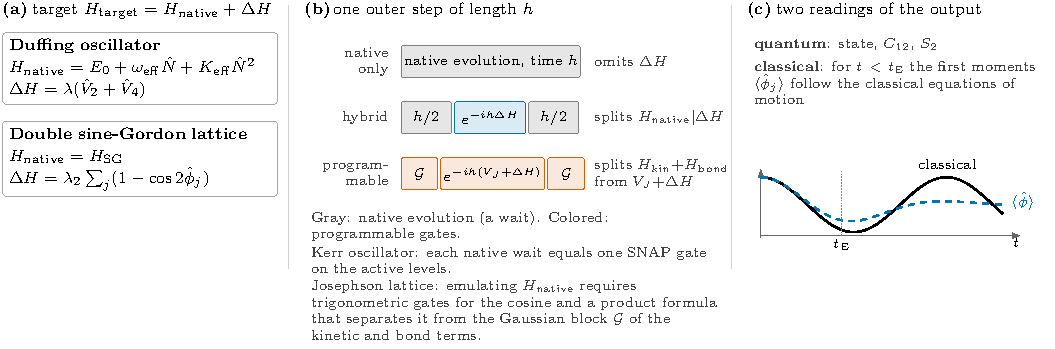
\includegraphics[width=\textwidth]{figures/fig_overview.pdf}
\caption{Native-plus-correction simulation. (a) The target Hamiltonian is split into a native part generated by the circuit and a correction \(\Delta H\). The two benchmarks with a correction differ in the type of native term. (b) One outer step of three implementations for the lattice. Native-only evolution omits the correction, a hybrid step brackets compiled gates for the correction by native half steps, and a programmable step emulates the native part as well, here by splitting the kinetic and bond terms, applied as one Gaussian block \(\mathcal G\), from the Josephson potential and the correction, \(V_J+\Delta H\) (Sec.~\ref{sec:dsg}). (c) The output is read either as a quantum state and its observables, such as the correlation \(C_{12}\) and entropy \(S_2\) of Sec.~\ref{sec:dsg}, or, through the first moments, as a classical trajectory that is valid only up to the mean-field validity time \(t_{\rm E}\) of Eq.~\eqref{eq:mean-field-validity-time}. Panel (c) is a schematic.}
\label{fig:overview}
\end{figure*}

\subsection{Josephson dictionaries and Hamiltonian flows}
\label{subsec:dictionaries}

We introduce a \emph{hardware-native nonlinearity dictionary}, a collection of nonlinear functions
$\mathcal D_{\rm hw} = \{\psi_\mu(\mathbf x) \}_{\mu\in\mathcal I},$
chosen so that each dictionary element corresponds to a native or parametrically activated nonlinear response of the underlying circuit. For Josephson-based hardware, the dictionary naturally includes trigonometric functions generated by the current-phase relation, polynomial nonlinearities arising from weakly anharmonic expansions, and multimode mixing terms generated by coupled nonlinear elements. Appendix~\ref{app:equation-classes} derives further dictionaries and the classes of nonlinear differential equations that they represent, and this subsection collects the elements used below.

A superconducting circuit containing a Josephson junction admits the quantized Hamiltonian
\begin{align}
\hat H_{JJ}=4E_C \hat n^2-E_J\cos\hat\phi,
\label{eq:jj-hamiltonian}
\end{align}
where \(\hat \phi\) and \(\hat n\) denote the superconducting phase and Cooper-pair number operators, respectively, and satisfy the canonical commutation relation
\([\hat\phi,\hat n]=i.\)
Here,
$E_C=\frac{e^2}{2C}, E_J=\frac{\hbar I_C}{2e},$
with \(C\) the junction capacitance and \(I_C\) the critical current.

The Josephson nonlinearity can be written exactly as
\(\cos\hat\phi=\frac{1}{2}\left(e^{i\hat\phi}+e^{-i\hat\phi}\right).\)
This structure motivates an \emph{exact Josephson dictionary}
\begin{align}
\mathcal D_{J}^{\rm exact}=\left\{I,\,\hat n,\,\hat n^2,\,e^{ik\hat\phi},\,e^{-ik\hat\phi}\,\right\}_{k\in\mathbb N},
\label{eq:exact-josephson-dictionary}
\end{align}
or, equivalently,
\begin{align}
\mathcal D_{J}^{\rm trig}=\left\{I,\,\hat n,\,\hat n^2,\,\cos(k\hat\phi),\,\sin(k\hat\phi)\right\}_{k\in\mathbb N}.
\label{eq:trig-josephson-dictionary}
\end{align}
For an ideal single junction, the fundamental harmonic \(k=1\) appears directly in the circuit Hamiltonian. Higher harmonics may be generated effectively by junction arrays, multijunction loops, multiphoton processes, or driven nonlinear interactions. This trigonometric dictionary is particularly natural when the target nonlinear vector field contains periodic functions, since the Josephson interaction provides such functions without first replacing them by a polynomial expansion.

In the transmon regime \(E_J\gg E_C\), fluctuations of the phase are localized near a minimum of the Josephson potential, and expanding the cosine gives the local polynomial dictionary of Appendix~\ref{app:equation-classes}.
Retaining the leading quartic correction and applying the rotating-wave approximation yields the familiar weakly anharmonic Kerr form
\begin{align}
\hat H_K\simeq\omega_q \hat N+\frac{K}{2}\hat a^{\dagger 2}\hat a^2,
\label{eq:kerr-hamiltonian}
\end{align}
where
$\hat N=\hat a^\dagger\hat a$
is the bosonic occupation-number operator. For the transmon,
\begin{align}
\omega_q\simeq\sqrt{8E_JE_C}-E_C,\qquad K\simeq -E_C,
\end{align}
in units where \(\hbar=1\), up to the convention used for the Kerr coefficient. Since
\(\hat a^{\dagger 2}\hat a^2=\hat N(\hat N-1),\)
the same Hamiltonian can be written as a polynomial in \(\hat N\),
\begin{align}
\hat H_K=\widetilde\omega\,\hat N+\widetilde K\,\hat N^2+{\rm const.}
\end{align}
This motivates a \emph{number-operator dictionary}
\begin{align}
\mathcal D_{J}^{N}=\left\{I,\,\hat N,\,\hat N^2,\,\hat N^3,\ldots\right\}.
\label{eq:number-dictionary}
\end{align}

For multiple coupled modes, the phase appearing across a nonlinear element generally contains contributions from several normal modes,
\(\hat\theta=\sum_{j=1}^{d}\eta_j\hat\phi_j+\phi_{\rm ext}.\)
The resulting Josephson term is
\begin{align}
\hat H_J^{(d)}=-E_J\cos\left(\sum_{j=1}^{d}\eta_j\hat\phi_j+\phi_{\rm ext}\right).
\label{eq:multimode-josephson}
\end{align}
This naturally generates nonlinear functions of several dynamical variables. Accordingly, we define the \emph{multimode Josephson dictionary}
\begin{align}
\mathcal D_{J}^{\rm mix}=\left\{\sin\left(\mathbf k\cdot\hat{\boldsymbol\phi}+\theta\right),\,\cos\left(\mathbf k\cdot\hat{\boldsymbol\phi}+\theta\right)\right\}_{\mathbf k,\theta},
\label{eq:multimode-dictionary}
\end{align}
where
$\hat{\boldsymbol\phi}=(\hat\phi_1,\ldots,\hat\phi_d)^T.$

The local polynomial dictionary \(\mathcal D_J^{\rm poly}\) and the flux-biased dictionary \(\mathcal D_J^{\rm bias}\), which describe small excursions about an operating point and flux-tunable three- and four-wave mixing, are defined in Appendix~\ref{app:equation-classes}.
Collecting these possibilities, the hardware-native nonlinear dictionary of a programmable Josephson platform may be written schematically as
\begin{align}
\mathcal D_{\rm SC}=\mathcal D_{J}^{\rm exact}\cup\mathcal D_{J}^{\rm poly}\cup\mathcal D_{J}^{N}\cup\mathcal D_{J}^{\rm bias}\cup\mathcal D_{J}^{\rm mix}.
\label{eq:complete-superconducting-dictionary}
\end{align}
These sets represent different descriptions of the nonlinear operator algebra accessible in distinct physical regimes. The exact trigonometric dictionary retains the full Josephson nonlinearity; the polynomial dictionary is appropriate for small excursions around a stable operating point; the number-operator dictionary describes the weakly anharmonic Kerr regime; and the multimode dictionary captures nonlinear interactions generated when several oscillator coordinates participate in the same Josephson element.

A closed circuit does not realize every vector field that these dictionaries represent, nor an arbitrary coefficient matrix \(C\) in their expansion (Appendix~\ref{app:equation-classes}). Its classical limit is a Hamiltonian flow in canonical coordinates \(\mathbf z=(\mathbf q,\mathbf p)\in\mathbb R^{2m}\),
\begin{align}
\mathbf f(\mathbf z)=J\nabla h(\mathbf z),\qquad J=\begin{pmatrix}0&I\\-I&0\end{pmatrix},
\label{eq:hamiltonian-flow}
\end{align}
and on a simply connected domain a \(C^1\) vector field has this form exactly when
\begin{align}
(D\mathbf f)^{T}J+J\,D\mathbf f=0.
\label{eq:realizability}
\end{align}
The dictionary expansion therefore applies to the Hamiltonian, \(h\approx\sum_\mu c_\mu\psi_\mu\), and every force component follows from derivatives of the same coefficients. For example, with \(M=M^T>0\), \(K=K^T\), and real \(E_\mu\), \(\mathbf k_\mu\), and \(\vartheta_\mu\),
\begin{align}
h={}&\tfrac12\mathbf p^{T}M^{-1}\mathbf p+\tfrac12\mathbf q^{T}K\mathbf q\nonumber\\
&+\sum_\mu E_\mu\big[1-\cos(\mathbf k_\mu\cdot\mathbf q+\vartheta_\mu)\big]
\label{eq:realizable-h}
\end{align}
generates \(\dot{\mathbf q}=M^{-1}\mathbf p\) and \(\dot{\mathbf p}=-K\mathbf q-\sum_\mu E_\mu\mathbf k_\mu\sin(\mathbf k_\mu\cdot\mathbf q+\vartheta_\mu)\), so the force coefficient of each harmonic is fixed by its wave vector. The field \((\dot q,\dot p)=(-q,0)\) violates Eq.~\eqref{eq:realizability}. Hardware realization imposes further conditions on the signs and ranges of the coefficients and on the coupling graph, for example \(K\succeq0\) for a passive inductive network. The condition refers to direct realization in these canonical coordinates and does not exclude enlarged encodings or open-system constructions. Among the vector fields that the dictionaries represent, the ones realized directly by a closed circuit are therefore the Hamiltonian flows with hardware-admissible coefficients, of which Eq.~\eqref{eq:realizable-h} is a typical form. First-order phase models such as the Kuramoto network and reaction--diffusion terms can be represented by the dictionaries but are dissipative and lie outside this unitary subclass (Appendix~\ref{app:equation-classes}).

Many equations of practical interest contain an additional linear dissipative contribution, such as the discretized diffusion operator in a reaction--diffusion model, which closed-system unitary evolution cannot generate. Appendix~\ref{app:lchs} describes a hybrid construction in which the nonlinear Hermitian sector remains native to the system hardware while a single ancillary oscillator supplies a linear positive-semidefinite nonunitary sector through a linear-combination-of-Hamiltonian-simulation (LCHS) dilation \cite{An_2023,An_2026,das2026quantumdifferentialequationsolver}. That construction acts on the Hilbert-space generator. Relating it to the first moments of a dissipative classical field requires a separate encoding argument, and the benchmarks in Sec.~\ref{sec:benchmarks} are unitary.

\subsection{Encoded field and the validity of the encoding}
\label{subsec:encoding}

Let the target be a classical nonlinear evolution equation for a field $u(x,t)$, semidiscretized on $N_{\rm site}$ points as $u_j(t)$. We assign one bosonic mode to each site and encode the field in the \emph{first moments} of the mode operators,
\begin{align}
u_j(t) \;\longleftrightarrow\; \langle \hat a_j(t)\rangle,
\qquad\text{or}\qquad
\bigl(u_j,\dot u_j\bigr) \;\longleftrightarrow\;
\bigl(\langle\hat q_j\rangle,\langle\hat p_j\rangle\bigr),
\label{eq:encoding}
\end{align}
according to whether the target equation is first or second order in time. No amplitude encoding is used: the field is not stored in the wavefunction amplitudes, and consequently the mode count scales linearly, not logarithmically, with $N_{\rm site}$.

For the Hermitian nonlinear sector, Heisenberg evolution generated by $\hat H_{\rm target}$ produces an open hierarchy in which the first moments couple to higher moments. Closing it at first order,
\(\bigl\langle f(\hat a^\dagger,\hat a)\bigr\rangle\;\approx\;f\bigl(\langle\hat a^\dagger\rangle,\langle\hat a\rangle\bigr),\)
yields the target classical equation. For arbitrary states, Hamiltonians of at most quadratic order close the first-moment equations exactly \cite{Adesso_2014}. Nonlinear Hamiltonians generally couple first moments to higher moments, although special states, symmetries, or restricted sectors may produce additional closures \cite{Plankensteiner_2022}.

In conventional semiclassical scalings the relative correction is often suppressed by $O(1/\bar n)$ (where $\bar n = \langle \hat N \rangle =\langle\hat a^\dagger\hat a\rangle$ denotes the mean occupation of a mode) \cite{Polkovnikov_2010}, but the precise power and prefactor depend on the Hamiltonian, state family, and observable. The discrepancy between the device and the classical target is therefore proportional to precisely the nonlinearity that motivates the construction. This is not a defect of the present scheme; it is a general property of encoding a classical field in the first moments of a quantum system, and it delimits where the classical reading of the dynamics applies \cite{Ballentine_1994}.

We present two illustrations, both realized in the examples below.
For the Josephson cosine, suppose that the spectral probability distribution of \(\hat\phi\) in the state is Gaussian, with mean \(\langle\hat\phi\rangle\) and variance \(\Delta\phi^2\) \cite{Adesso_2014}. Its characteristic function then gives
\begin{align}
\bigl\langle \sin\hat\phi\bigr\rangle=e^{-\Delta\phi^2/2}\,\sin\bigl\langle\hat\phi\bigr\rangle,
\label{eq:debye-waller}
\end{align}
so the dimensionless onsite coefficient entering the mean-field equation is renormalized to $E_J e^{-\Delta\phi^2/2}$.
Here
\(\Delta\phi^2 \equiv \bigl\langle\hat\phi^2\bigr\rangle- \bigl\langle\hat\phi\bigr\rangle^2\)
is the variance of the phase quadrature. Zero-point fluctuations therefore weaken the nonlinear restoring force by an amount set entirely by the oscillator's phase spread.

For the Kerr oscillator of Sec.~\ref{sec:duffing},
a coherent state \(\ket{\alpha}\) with \(\bar n=|\alpha|^2\) evolves with first moment \cite{Milburn1986,YurkeStoler1986}
\[
\bigl|\langle\hat a(t)\rangle\bigr|  = \sqrt{\bar n}\, \exp\!\bigl[ \bar n\bigl(\cos(2K_{\rm eff}t)-1\bigr) \bigr].
\]
For \(K_{\rm eff}\neq0\) and \(\bar n>0\), its small-time envelope is
\[
\bigl|\langle\hat a(t)\rangle\bigr| = \sqrt{\bar n}\, \exp\!\bigl[ -2\bar n K_{\rm eff}^2t^2+\mathcal O(t^4)\bigr],
\]
so the \(e^{-1}\) collapse timescale is
\(t_{\rm c}\simeq (|K_{\rm eff}|\sqrt{2\bar n})^{-1}.\)
The magnitude first returns at \(t_{\rm rev}=\pi/|K_{\rm eff}|\). At intermediate times it can be exponentially suppressed while the corresponding classical amplitude remains \(\mathcal O(1)\), even though no energy has been lost.

The phase variance \(\Delta\phi^2\) and the Kerr collapse estimate \(t_{\rm c}\) are model-specific diagnostics. For each benchmark compared with a classical reference, let \(d_{\rm MF}(t)\) be a normalized first-moment discrepancy defined for that benchmark and let \(\varepsilon_{\rm MF}^{\star}\) be the corresponding tolerance. We define
\begin{align}
t_{\rm E} \equiv \inf\left\{ t\geq0: d_{\rm MF}(t)>\varepsilon_{\rm MF}^{\star} \right\}, \qquad \inf\varnothing=\infty .
\label{eq:mean-field-validity-time}
\end{align}
For a finite observation horizon \(T\), absence of a threshold crossing is reported as \(t_{\rm E}>T\).
For each benchmark we give \(d_{\rm MF}\), \(\varepsilon_{\rm MF}^{\star}\), and the observation horizon. The Kerr quantity \(t_{\rm c}\) is reported separately and is identified with \(t_{\rm E}\) only when the same threshold test establishes that relation. Throughout we use \(\varepsilon_{\rm MF}^{\star}=0.10\) and locate a crossing on the sampled time grid by linear interpolation within its bracketing interval.

Accordingly we distinguish:
\begin{itemize}
\item \emph{Mean-field regime} (\(t\lesssim t_{\rm E}\), typically \(\bar n\gg1\)). The first moments agree with the classical reference within \(\varepsilon_{\rm MF}^{\star}\). We use this regime for validation and claim no advantage in it.
\item \emph{Beyond-mean-field regime} (\(t\gtrsim t_{\rm E}\), typically \(\bar n=O(1)\)). The processor realizes the cutoff quantum model. An exact dense state-vector representation has dimension \(n_{\rm cut}^{N_{\rm site}}\).
\end{itemize}

A Gronwall estimate, Eq.~\eqref{eq:classical-transfer} of Appendix~\ref{app:proofs}, bounds the distance between the first moments of the exact finite quantum model and the classical trajectory by the integrated closure residual, the cutoff residual, and the dictionary error. An implemented state within projective distance \(\epsilon_q\) of the exact finite state, as defined in Sec.~\ref{subsec:error-bounds}, shifts each first moment by at most \(2\max_j\|\hat Z_j\|_2\,\epsilon_q\), where \(\hat Z_j\) are the quadratures on the truncated space. The closure residual is not small beyond the mean-field regime, so the classical reading can fail even when the quantum implementation is exact, and Sec.~\ref{sec:benchmarks} measures \(t_{\rm E}\) directly.

\subsection{Native match and correction}
\label{subsec:native-match}

We write the Hermitian target as
\begin{align}
H_{\rm target}&=H_{\rm native}+\Delta H,\nonumber\\
H_{\rm native}&=\sum_{\mu=1}^{M}c_{\mu}D_{\mu},\qquad D_{\mu}\in\mathcal D_{\rm SC},
\label{eq:native-hamiltonian-dictionary}
\end{align}
where each \(D_{\mu}\) is a native or parametrically activated superconducting interaction. The correction \(\Delta H=H_{\rm target}-H_{\rm native}\) contains any residual contribution that is not captured exactly by the chosen finite hardware dictionary. Depending on the implementation, \(\Delta H\) may either be synthesized separately or neglected and treated as a controlled dictionary-approximation error. Although \(H_{\rm native}\) may contain strongly nonlinear operators such as \(\cos\hat\phi\), \(\hat X^3\), \(\hat X^4\), and \(\hat N^2\), it is still a fixed Hermitian operator on the cutoff-restricted system Hilbert space.

\paragraph{Phase-insensitive Hamiltonian mismatch.}
Because adding a scalar multiple of the identity to a Hermitian Hamiltonian changes only the global phase of unitary evolution, Hamiltonian mismatch diagnostics should be insensitive to the arbitrary choice of energy zero. For a Hermitian operator \(X\) on a finite space, define
\begin{align}
c(X)=\frac{\lambda_{\max}(X)+\lambda_{\min}(X)}{2},\qquad X_\circ=X-c(X)I .
\label{eq:energy-zero-convention}
\end{align}
The centered representative removes the optimal scalar energy offset in the spectral norm.

The phase-insensitive native mismatch is then defined by
\begin{align}
\eta_H\equiv\frac{\|\Delta H_\circ\|_2}{\|(H_{\rm target})_\circ\|_2},\qquad\|(H_{\rm target})_\circ\|_2>0,
\label{eq:phase-invariant-eta}
\end{align}
where the centering is applied consistently to the target and residual mismatch. Thus \(\eta_H\) measures the residual generator mismatch after removing physically irrelevant scalar energy offsets. When \(\Delta H=0\), the ideal native mismatch vanishes exactly. For the unbounded oscillator Hamiltonians used below, the norms refer to the stated numerical cutoff and grow with it.

\paragraph{Correction and splitting diagnostics.}
The noncommutativity introduced by the residual Hermitian sector is characterized by
\begin{align}
C_{\rm corr}\equiv\|[H_{\rm native},\Delta H]\|_2, \qquad C_{\rm LCHS}\equiv\|[L_{\rm lin},H_{\rm target}]\|_2 .
\label{eq:combined-cost-diagnostics}
\end{align}
The first quantity measures the degree to which the native nonlinear evolution and the programmable Hermitian correction fail to commute, and therefore serves as a diagnostic for the leading-order error introduced by splitting these two sectors. The second quantifies the noncommutativity between the linear nonunitary generator \(L_{\rm lin}\) of Appendix~\ref{app:lchs} and the complete Hermitian target sector, providing the corresponding diagnostic for LCHS/product-formula splitting. These quantities are not intended to replace complete product-formula error bounds, which may also depend on evolution time and higher-order nested commutators \cite{Childs2021Trotter}. In numerical studies they are evaluated in a finite Fock representation at the stated cutoff. For unbounded generators they grow with that cutoff (Appendix~\ref{app:class-diagnostics}). State-dependent product-formula bounds for unbounded operators avoid this growth \cite{AnFangLin2021,Sahinoglu2021,Burgarth2024Strong}, and the accuracy claims below rest on the state-dependent bounds of Sec.~\ref{subsec:error-bounds} and on direct simulation.

\paragraph{Classes of native match.}
A native-match criterion is meaningful only relative to a specified dynamical accuracy target. For a benchmark \(B\) with maximum trajectory infidelity \(\mathcal I_{\rm traj}^{\star}\), amplitude budget \(\epsilon_{\rm traj}^{\star}=\sqrt{\mathcal I_{\rm traj}^{\star}}\), and evolution time \(T\), the uniform bound of Theorem~\ref{thm:native-residual} shows that native evolution alone stays within one third of the budget on every input when \(T\|\Delta H_\circ\|_2\le\epsilon_{\rm traj}^\star/3\). The Hermitian sector then has a Class I native match. It is natively approximated, or Class II, when this condition fails but \(\eta_H<1\), and models with \(\eta_H\geq1\) lie outside both classes, since the native sector is not a leading approximation there. Throughout we use \(\mathcal I_{\rm traj}^\star=10^{-3}\). The one-third split fixes only this classification threshold. Circuit acceptance in Sec.~\ref{sec:benchmarks} instead adds the synthesis error and the numerical margins and compares the sum with the full \(\epsilon_{\rm traj}^\star\) (Appendix~\ref{app:numerics}). Appendix~\ref{app:native-match} writes the condition as a tolerance on \(\eta_H\), states the definitions formally, and gives a hardware-calibrated variant that adds calibration and model uncertainty to the mismatch.

The label Class I or Class II characterizes the Hermitian sector only. We append U when $L_{\rm lin}=0$ and N when $L_{\rm lin}\neq0$ is implemented through the ancillary-mode LCHS construction of Appendix~\ref{app:lchs}. Table~\ref{tab:classes} lists the class of each benchmark, and the classes differ in where the cost sits.

Class I carries a constraint absent from a fully digital implementation: its accessible parameters are restricted by fabrication values and by the available bias, drive, and parametric control ranges. They are not arbitrarily programmable. For Class I--U, the compiled logical depth of the evolution block may be independent of simulated time, although the native analog waiting time grows linearly with physical evolution time. For Classes I--N and II--N, the LCHS kernel preparation, hybrid evolution, and postselection introduce additional depth and sampling costs even when the nonlinear Hermitian sector is exactly native. A class label is a statement about the operator-level mismatch and does not by itself order the resource cost of two implementations, which requires a common accuracy criterion and the resource accounting of Sec.~\ref{sec:benchmarks}.

Both class conditions refer to the stated cutoff. For an unbounded correction \(T\|\Delta H_\circ\|_2\) grows without limit with the cutoff, so the target leaves Class I at a large enough cutoff whatever the effect of the correction on the states of interest. The ratio \(\eta_H\) does not measure that effect either. In the double sine-Gordon example of Sec.~\ref{sec:dsg} it is 0.008 at local cutoff 48, while native-only evolution departs from the target state by up to 0.41. The effect of a correction on specified inputs is measured by Theorem~\ref{thm:native-residual} and by direct simulation.

\subsection{Error of an omitted or compiled correction}
\label{subsec:error-bounds}

For normalized pure states we use the projective distance and the infidelity,
\begin{align}
\dpr(\psi,\varphi)=\min_{\theta\in\mathbb R}\|\psi-e^{i\theta}\varphi\|,\qquad \mathcal I=1-|\langle\psi|\varphi\rangle|^2 .
\label{eq:metrics}
\end{align}
They obey \(\mathcal I=\dpr^2(1-\dpr^2/4)\le\dpr^2\), so amplitude errors from different sources are added before conversion to an infidelity. For a bounded observable \(O\), \(|\langle\psi|O|\psi\rangle-\langle\varphi|O|\varphi\rangle|\le2\|O\|_2\,\dpr(\psi,\varphi)\).

\begin{theorem}[Native-reference residual bound]
\label{thm:native-residual}
Let \(H=H_0+R\) with \(H_0\) and \(R\) Hermitian on a finite-dimensional space, let \(\|\psi_0\|=1\), and set \(\psi_0(t)=e^{-itH_0}\psi_0\) and \(\psi(t)=e^{-itH}\psi_0\). With \(a(s)=\langle\psi_0(s)|R|\psi_0(s)\rangle\),
\begin{align}
\dpr\big(\psi(t),\psi_0(t)\big)\le B_\psi(t)\equiv\int_0^t\big\|\big(R-a(s)\big)\psi_0(s)\big\|\,ds ,
\label{eq:native-residual}
\end{align}
and hence \(\mathcal I(t)\le\min\{1,B_\psi(t)^2\}\). Uniformly over inputs, \(\min_\theta\|e^{-itH}-e^{i\theta}e^{-itH_0}\|_2\le t\|R_\circ\|_2\).
\end{theorem}

The integrand is the standard deviation of the omitted correction in the native reference state, so the bound vanishes for \(R\propto I\) and ignores any part of \(R\) that acts on the reference trajectory as a phase. The phase-agnostic residual method of Ref.~\cite{Zoufal2023}, the state-dependent step analysis of Ref.~\cite{Hatomura2022}, and state-dependent product-formula bounds \cite{AnFangLin2021,Burgarth2024Strong} rest on the same Duhamel estimate. The reference here is the trajectory of an available native Hamiltonian, which makes \(B_\psi\) an input-specific test of whether a given correction can be omitted. For an infidelity threshold \(\mathcal I_\star\) the test has three outcomes. Native-only evolution is \emph{sufficient} when \((B_\psi+\epsilon_{\rm num})^2\le\mathcal I_\star\), where \(\epsilon_{\rm num}\) collects the numerical margins of the evaluation. It \emph{fails} when a directly computed infidelity exceeds \(\mathcal I_\star\) by more than its numerical uncertainty. Otherwise the test is \emph{inconclusive}, and a large bound alone does not show that the correction is needed. Evaluating \(B_\psi\) requires the native trajectory, which is inexpensive for number-diagonal native Hamiltonians and generally as hard as the simulation itself for a coupled native lattice. Appendix~\ref{app:proofs} gives the proof.

A compiled step \(W\) of length \(h\) approximates the exact step \(U=e^{-ihH_{\rm target}}\) on the same finite space. For any phase \(\theta\) fixed for all steps and inputs,
\begin{align}
\dpr\big(W^r\psi,U^r\psi\big)\le\sum_{k=0}^{r-1}\big\|(W-e^{i\theta}U)\,U^k\psi\big\| ,
\label{eq:action-sum}
\end{align}
which we call the composition bound. It follows from telescoping (Appendix~\ref{app:proofs}), and its right-hand side requires the action of the compiled step only on the exact intermediate states \(U^k\psi\), not on the whole Hilbert space. A small training loss on initial states does not control these terms, which becomes important in Sec.~\ref{subsec:df-compile}. When the step uses an ancillary qubit that starts in \(\ket{0}\), Eq.~\eqref{eq:action-sum} holds with \(U\otimes I\) acting on \(U^k\psi\otimes\ket{0}\), and tracing out the qubit cannot increase the Bures distance \(d_B=\sqrt{2-2\sqrt F}\) with \(F=\langle\psi_{\rm ref}|\rho_{\rm sys}|\psi_{\rm ref}\rangle\), which reduces to \(\dpr\) for pure states.

\subsection{Programmable resources}
\label{subsec:resources}

\paragraph{Programmable primitives and resource accounting.}
The programmable primitive set \(\mathcal P\) is defined as the collection of externally controlled operations that are actively invoked to synthesize the non-native portion of the target dynamics. The set is platform dependent and may include, depending on the hardware realization, single-mode displacements, SNAP phases, squeezing operations, qubit rotations, dispersive controls, Gaussian two-mode hopping or gradient operations, and system-number-controlled ancillary displacements. Only operations contained in \(\mathcal P\) and explicitly used in a benchmark contribute to the programmable resource cost.

The resource accounting distinguishes between programmable and native contributions. We denote by \(G_{\rm step}\) the number of programmable primitive segments per simulation step and by \(D_{\rm step}\) their parallel depth. The corresponding full-trajectory quantities are obtained by summing over all simulation steps. Native analog evolution generated by \(H_{\rm native}\) is not included in \(G_{\rm step}\) or \(D_{\rm step}\), since it represents the hardware-native resource advantage. Instead, its contribution is characterized through the available evolution time, physical parameters, and native-match diagnostics. Resource tables therefore report programmable operation counts, native waits, and ancillary resources separately rather than combining physically distinct resources into a single gate count, and Sec.~\ref{subsec:duration} discusses depth and duration. The counts also leave out the classical cost of compiling a block. That cost vanishes for gates with analytic parameters, such as the SNAP phases of a Kerr evolution and the trigonometric gates of Sec.~\ref{sec:dsg}, and is substantial for numerically optimized blocks, such as the SNAP-plus-displacement circuits of Sec.~\ref{subsec:df-compile}.

\paragraph{Emulation cost of a native interaction.}
The saving from native evolution is measured against a programmable emulation of the same evolution, and the strongest available emulation determines it. When \(H_{\rm native}\) is diagonal in the number basis, as for a Kerr mode, one SNAP gate reproduces a native wait of any duration on the levels it addresses \cite{Krastanov_2015,Heeres_2015}, so native evolution saves at most one programmable operation per wait (Sec.~\ref{subsec:df-compile}). When \(H_{\rm native}\) contains noncommuting quadrature functions, as for a Josephson lattice, its emulation requires trigonometric gates for the cosine and a product formula that separates the cosine from the kinetic energy. Native evolution then removes the cosine from the compiled part and its commutators from the splitting error, whereas the quadratic kinetic and bond terms can be emulated as one Gaussian block, exactly for canonical operators (Sec.~\ref{sec:dsg}). The dictionaries of Sec.~\ref{subsec:dictionaries} differ in this respect. Elements of the number-operator dictionary \(\mathcal D_J^{N}\) are emulated exactly by SNAP phases on a finite set of levels, whereas the cosine and sine elements of \(\mathcal D_J^{\rm trig}\) and \(\mathcal D_J^{\rm mix}\) are not diagonal in the number basis and do not commute with the kinetic terms.

\paragraph{Resource-bounded simulability.}
Appendix~\ref{app:simulability} collects these resources, together with the ancillary oscillators and the sampling overhead of the nonunitary construction of Appendix~\ref{app:lchs}, in a definition of resource-bounded hybrid simulability.

\section{Benchmarks}
\label{sec:benchmarks}

The three detailed examples below lie on the unitary boundary of the general generator-level framework. For all of them, $L_{\rm lin}=0,$ so the one-oscillator LCHS block is inactive and no recovery postselection is required. They isolate the classification of the Hermitian nonlinear sector. The sine-Gordon lattice is Class I--U because its Hamiltonian is generated directly, whereas the Duffing oscillator and the deformed (double) sine-Gordon lattice are Class II--U. Class I--N and Class II--N models add a linear accretive sector implemented through the one-oscillator LCHS block (Appendix~\ref{app:lchs}).

All results are computed on truncated Fock spaces whose cutoffs are stated with each result. States from different cutoffs are compared after zero padding, and the changes between adjacent cutoffs, time steps, and circuit paddings are reported as empirical numerical margins rather than rigorous bounds. Appendix~\ref{app:numerics} describes the numerical methods, and Appendix~\ref{app:lean} lists the statements that are formally verified in Lean. Circuit comparisons use ideal primitives and treat native evolution for a chosen time as one switchable operation, and Sec.~\ref{subsec:hardware} discusses what this assumes about the device.

\subsection{Sine-Gordon lattice}
\label{sec:sg}

The sine-Gordon lattice belongs to Class I--U. Its target generator is purely Hermitian.
No LCHS ancillary oscillator, LCHS kernel preparation, or postselection is required. The Josephson cosine and the intersite circuit couplings generate the target Hamiltonian directly.

Because the nonlinear Hamiltonian is supplied directly by the native analog hardware, no programmable nonlinear correction layer or Hermitian-sector product formula is required. Accordingly \(\Delta H=0\) and \(\eta_H=C_{\rm corr}=0\) at every cutoff. The class holds by construction, since the target is defined as the circuit Hamiltonian, and the benchmark tests the classical reading of the native dynamics.

\subsubsection{The model and its circuit realization}
\label{subsec:sg-model}

The $(1+1)$-dimensional sine-Gordon equation for a real scalar field $\phi(x,t)$ is
\begin{align}
\partial_{tt}\phi(x,t) - c^2\partial_{xx}\phi(x,t) + \omega_J^2\sin\phi(x,t) = 0,
\label{eq:sinegordon}
\end{align}
where $x$ is the spatial coordinate, $t$ is time, $\phi(x,t)$ is the dimensionless sine-Gordon field, $c$ is the characteristic propagation velocity, and $\omega_J$ sets the local nonlinear oscillation frequency. The notation $\partial_{tt}\phi$ and $\partial_{xx}\phi$ denotes the second derivatives of the field with respect to time and space, respectively.
This equation is generated by the Hamiltonian density
\begin{align}
\mathcal H =\tfrac12\Pi^2+ \tfrac{c^2}{2}(\partial_x\phi)^2+ \omega_J^2\bigl(1-\cos\phi\bigr),
\label{eq:sg-density}
\end{align}
where $\mathcal H(x,t)$ is the energy density and $\Pi(x,t)$ is the canonical momentum conjugate to $\phi(x,t)$. In the normalization used here, $\Pi=\partial_t\phi$. The first term is the local kinetic-energy density, the second penalizes spatial variations of the field, and the third is the periodic sine-Gordon potential. To obtain a finite-dimensional lattice model, the spatial coordinate is discretized as \(x_j=jb\), \(j=1,\ldots,N_{\rm site}\), where $N_{\rm site}$ is the number of lattice sites, $b$ is the lattice spacing, and $j$ labels the individual sites. The continuum fields are then replaced by site variables, \(\phi_j(t)\equiv \phi(x_j,t)\) and \(\Pi_j(t)\equiv \Pi(x_j,t)\), with $\phi_j$ and $\Pi_j$ forming a canonical conjugate pair at site $j$. Using a nearest-neighbor finite-difference approximation for the spatial derivative, and after the standard rescaling of the lattice variables to canonical oscillator units, the discretized Hamiltonian takes the form
\begin{align}
H_{\rm SG} ={}&\sum_{j} \left[ \tfrac{\Pi_j^2}{2} + E_J\bigl(1-\cos\phi_j\bigr) \right]\nonumber\\
&+ \tfrac{\kappa}{2}\sum_{j}\bigl(\phi_{j+1}-\phi_j\bigr)^2,\qquad\kappa \equiv \tfrac{c^2}{b^2}.
\label{eq:sg-lattice}
\end{align}
Here, $H_{\rm SG}$ is the total lattice Hamiltonian, $E_J$ is the dimensionless strength of the onsite periodic potential in the convention adopted below, and $\kappa$ is the nearest-neighbor coupling strength. The quantity $\phi_{j+1}-\phi_j$ measures the field difference between adjacent sites, so the coupling term suppresses rapid spatial variation across the lattice. The precise range of the nearest-neighbor sum depends on the imposed boundary conditions; for example, periodic boundaries identify $\phi_{N_{\rm site}+1}$ with $\phi_1$, whereas open boundaries include only the $N_{\rm site}-1$ physical links. The onsite cosine interaction and the quadratic coupling terms therefore constitute the complete target Hermitian generator; no additional programmable nonlinear correction is required.

For an interior site, or with indices interpreted periodically, Hamilton's equations generated by Eq.~\eqref{eq:sg-lattice} are
\(\dot{\phi}_j = \Pi_j\) and \(\dot{\Pi}_j= -E_J\sin\phi_j+ \kappa\left(\phi_{j+1}-2\phi_j+\phi_{j-1}\right)\), or, equivalently,
\begin{align}
\ddot{\phi}_j- \kappa\left(\phi_{j+1}-2\phi_j+\phi_{j-1}\right)+ E_J\sin\phi_j = 0.
\end{align}
Since
$\tfrac{\phi_{j+1}-2\phi_j+\phi_{j-1}}{b^2}\longrightarrow \partial_{xx}\phi(x,t)$
as $b\rightarrow0$, the lattice equations recover Eq.~\eqref{eq:sinegordon} in the continuum limit, with the onsite coefficient identified according to the chosen dimensionless normalization, typically $E_J\leftrightarrow\omega_J^2$.

For a circuit description, let $\hat n_j$ denote the Cooper-pair number operator, $[\hat\phi_j,\hat n_k]=i\delta_{jk}$, and write the physical Hamiltonian as
\begin{align}
H_{JJ}={}&\sum_j\left[4E_C\hat n_j^2+E_J^{\rm phys}(1-\cos\hat\phi_j)\right]\nonumber\\
&+\tfrac{E_L}{2}\sum_{\langle j,k\rangle}(\hat\phi_j-\hat\phi_k)^2.
\label{eq:jj-array}
\end{align}
Dividing by $8E_C$ gives Eq.~\eqref{eq:sg-lattice} with
\(\hat\Pi_j=\hat n_j\), \(E_J=\tfrac{E_J^{\rm phys}}{8E_C}\), and \(\kappa=\tfrac{E_L}{8E_C}\).
The dimensionless simulation time \(t\) and the laboratory time are related by
\(t=\tfrac{8E_C}{\hbar}\,t_{\rm lab}.\)
Thus \(E_J^{\rm phys}\) denotes the physical Josephson energy, whereas \(E_J\) denotes the dimensionless onsite coefficient used below.
Josephson-junction arrays are established realizations of discrete sine-Gordon dynamics and fluxon propagation \cite{Ustinov1995DiscreteSG,Ustinov1998Solitons}, and Josephson circuits have been proposed as analog simulators of the quantum sine-Gordon model \cite{Roy2021}. Here the lattice calibrates the classical reading of native evolution, and Sec.~\ref{sec:dsg} compares native evolution with programmable synthesis for its double sine-Gordon deformation.

The oscillator representation used below treats each \(\hat\phi_j\) as an extended coordinate whose spectrum is the real line. This is exact when every node is connected inductively, as in an inductively shunted junction \cite{Manucharyan2009Fluxonium,Koch2009Rf}. The shunt then adds an onsite quadratic term to Eq.~\eqref{eq:jj-array}, which changes the target by a Gaussian term but not its class, and the benchmarks below omit it. In an array whose nodes reach ground only through junctions, the total charge is quantized and the collective phase is compact. The extended model then remains accurate while phase slips between neighboring minima of the cosine are negligible, which requires \(E_J^{\rm phys}\gg E_C\) and excursions well inside one potential well. Results at \(E_J\lesssim1\), that is \(E_J^{\rm phys}/E_C\lesssim8\), therefore describe the extended-phase model.

\subsubsection{Quantization, encoding, and the semiclassical parameter}
\label{subsec:sg-quantization}

Representing each site by a bosonic mode of basis frequency $\omega_b$,
\begin{align}
\hat\phi_j = \tfrac{\hat a_j + \hat a_j^\dagger}{\sqrt{2\omega_b}},\qquad\hat\Pi_j = i\sqrt{\tfrac{\omega_b}{2}}\bigl(\hat a_j^\dagger - \hat a_j\bigr).
\label{eq:sg-quadratures}
\end{align}
The parameter \(\omega_b\) defines the oscillator representation and does not modify the physical Hamiltonian. These definitions satisfy the canonical relation for \(\omega_b>0\). For the classical-calibration scan below, we choose \(\omega_b=\Omega\equiv\sqrt{E_J+2\kappa}\) as a basis scale. This choice corresponds to the local curvature of the harmonicized lattice Hamiltonian around \(\phi_j=0\), where the coupling contributes two nearest-neighbor restoring terms. For the two-site open chain used below, each site has one neighbor, and \(\Omega\) is the harmonic frequency of the antisymmetric normal mode, whereas the symmetric mode has harmonic frequency \(\sqrt{E_J}\). This is a basis convention, not a proof that the choice globally minimizes the required cutoff. Cutoff convergence is checked numerically.

Following Sec.~\ref{subsec:encoding}, the encoded classical field is $\phi_j(t) \leftrightarrow \langle\hat\phi_j(t)\rangle$, and the classical lattice equation is recovered only under the mean-field closure. The closure neglects higher moments of the quantum field, in particular the difference between \(\langle\sin\hat\phi_j\rangle\) and \(\sin\langle\hat\phi_j\rangle\).
For the coherent-state initialization, the zero-point phase variance is
\(\Delta\phi^2 = 1/(2\omega_b).\)
For the calibration choice \(\omega_b=\sqrt{E_J+2\kappa}\), this becomes \(\Delta\phi^2=1/(2\sqrt{E_J+2\kappa})\). Substituting this initial value into Eq.~\eqref{eq:debye-waller} gives the initial-state Debye--Waller diagnostic
\begin{align}
\bigl\langle\sin\hat\phi_j\bigr\rangle= e^{-\tfrac{\Delta\phi^2}{2}}\,\sin\langle\hat\phi_j\rangle\qquad\text{(Gaussian states)}.
\label{eq:sg-dw}
\end{align}
Increasing \(E_J\) at fixed \(\kappa\) decreases the initial zero-point phase spread in this basis and generally suppresses fluctuation-induced renormalization near the harmonic minimum. At \(E_J=O(1)\), the fluctuation correction is substantial and the finite quantum dynamics must be checked directly.

For an uncoupled site, $E_J=\tfrac{E_J^{\rm phys}}{8E_C}$ is the circuit classicality parameter. Transmon-like ratios $\tfrac{E_J^{\rm phys}}{E_C}\sim50$--$100$ correspond to $E_J\sim6$--$12$, whereas ratios of order unity place the site in a strong-fluctuation regime. In an array, however, $\kappa$, boundary conditions, and collective modes also affect the fluctuation scale, so $E_J$ alone is not a complete phase-diagram coordinate.

\subsubsection{Validation against the classical field}
\label{subsec:sg-classical}

\begin{figure*}[t]
\centering
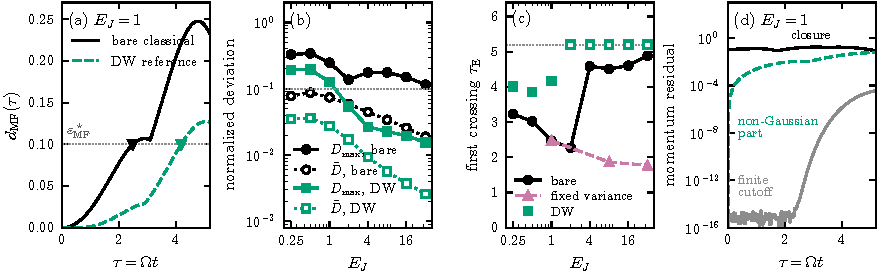
\includegraphics[width=\textwidth]{figures/fig_sg_classical.pdf}
\caption{Classical-field calibration of the two-site quantum sine-Gordon lattice (open boundaries, \(\kappa=1\), initial first moments \((1,0)\), local cutoff 80). Deviations are normalized by the classical oscillation amplitude \(A\), and time by \(\Omega=\sqrt{E_J+2\kappa}\). (a) Pointwise deviation of the quantum first moments from the bare classical and Debye--Waller (DW) references at \(E_J=1\), with triangles at the first crossings of \(\varepsilon^\star_{\rm MF}=0.1\) (dotted). (b) Maximum (filled) and mean (open) normalized deviations over the scan, with \(\varepsilon^\star_{\rm MF}\) dotted. (c) First crossing times for the primary preparation, \(\omega_b=\Omega\), and for the fixed-variance preparation \(\omega_b=\sqrt3\), which coincides with the primary one at \(E_J=1\). Open squares mark Debye--Waller references that do not cross before the end of the window at \(\tau=5.2\) (dotted). (d) Largest closure residual \(E_J|\langle\sin\hat\phi_j\rangle-\sin\langle\hat\phi_j\rangle|\) of the momentum equation over the two sites at \(E_J=1\), its non-Gaussian part \(E_J|\langle\sin\hat\phi_j\rangle-e^{-{\rm Var}\,\phi_j/2}\sin\langle\hat\phi_j\rangle|\), and the residual of the finite-cutoff commutator, with values below \(10^{-16}\) drawn at \(10^{-16}\).}
\label{fig:sg-classical-validation}
\end{figure*}

Because the identification $\phi_j(t)\leftrightarrow\langle\hat\phi_j(t)\rangle$ holds only under a mean-field closure, the first quantitative task is to locate the regime in which that closure is accurate. For open boundaries the classical reference is
\begin{align}
\ddot\phi_j=\kappa\sum_{k\in{\rm nn}(j)}(\phi_k-\phi_j)-E_J\sin\phi_j,
\label{eq:sg-classical-eom}
\end{align}
where the neighbor set contains one site at each endpoint and two in the interior, so that the bulk three-point stencil is not applied incorrectly at an open boundary. We compare this reference against numerically converged finite-cutoff evolution of Eq.~\eqref{eq:sg-lattice}, with the classical initial data matched to the state actually represented in the truncated oscillator basis,
\(\phi_j^{\rm cl}(0)=\langle\hat\phi_j(0)\rangle_{n_{\rm cut}}\) and \(\dot\phi_j^{\rm cl}(0)=\langle\hat\Pi_j(0)\rangle_{n_{\rm cut}}\),
rather than to the infinite-dimensional coherent-state parameters. We additionally integrate a \emph{fluctuation-renormalized} (Debye--Waller) reference in which the initial variance \(\Delta\phi^2(0)\) is used to replace \(E_J\) by $E_Je^{-\Delta\phi^2/2}$ \cite{PhysRevLett.49.681}, testing the leading Gaussian correction of Eq.~\eqref{eq:sg-dw}. That correction is not expected to remain accurate once the evolving state becomes non-Gaussian or develops intersite correlations.

To quantify the validity of the mean-field identification, the comparison must distinguish physical disagreement from trivial differences in scale. The relevant quantity is therefore not the absolute field deviation alone, but the deviation of the quantum first moment from the corresponding classical trajectory,
\(\langle\hat\phi_j(t)\rangle-\phi_j^{\rm cl}(t).\)
Because the characteristic oscillation frequency and field amplitude vary substantially across the \(E_J\) parameter sweep, we report errors using dimensionless quantities. The evolution time is scaled by a harmonic frequency of the lattice, and the field error is normalized by the classical oscillation amplitude. We use a maximum deviation to characterize the earliest and worst-case breakdown of the mean-field description and an average deviation to quantify the typical trajectory disagreement over all sites and times.

\paragraph{Metrics.}
The numerical scan uses two sites with open boundaries, \(\kappa=1\), initial first moments \((\phi_1,\phi_2)=(1,0)\) and \((\Pi_1,\Pi_2)=(0,0)\) in a product coherent state, and \(E_J\in\{0.25,0.5,1,2,4,8,16,32\}\). Each point is computed at local cutoffs \(n_{\rm cut}=48\), 64, and 80, and adjacent cutoffs are compared. Because the harmonic frequency
\(\Omega=\sqrt{E_J+2\kappa}\)
varies from \(1.50\) to \(5.83\) over this range, comparisons are performed at a fixed scaled evolution horizon,
\(\tau_{\max}=\Omega T=5.2,\)
or equivalently
\(T(E_J)=5.2/\sqrt{E_J+2\kappa} .\)
This choice fixes the number of periods of the antisymmetric normal mode, about 0.83. Within the same window the symmetric mode completes between 0.28 of its harmonic period at \(E_J=0.25\) and 0.80 at \(E_J=32\).

The field-error normalization is obtained from the classical reference trajectory,
\[
A=\max_j\frac{\max_\tau\phi_j^{\rm cl}(\tau)-\min_\tau\phi_j^{\rm cl}(\tau)}{2},
\]
which accounts for the variation of oscillation amplitude across the parameter sweep. Defining
\(\delta\phi_j^{({\rm ref})}(\tau)=\langle\hat\phi_j(\tau)\rangle-\phi_j^{\rm ref}(\tau),\)
we report the maximum and mean normalized deviations,
\begin{align}
D_{\max}^{({\rm ref})}&=\max_{\tau,j}\frac{|\delta\phi_j^{({\rm ref})}(\tau)|}{A},\nonumber\\
\overline D^{({\rm ref})}&=\left\langle\frac{|\delta\phi_j^{({\rm ref})}(\tau)|}{A}\right\rangle_{\tau,j}.
\label{eq:sg-Dbar}
\end{align}
The maximum deviation captures the earliest or worst-case breakdown of the mean-field trajectory, whereas the averaged deviation measures the typical agreement over the full lattice and evolution window.

For the mean-field validity threshold, the primary comparison is made against the bare classical solution of Eq.~\eqref{eq:sg-classical-eom},
\(d_{\rm MF}^{\rm SG}(\tau)=\max_j|\langle\hat\phi_j(\tau)\rangle-\phi_j^{\rm cl}(\tau)|/A,\)
with the prescribed tolerance \(\varepsilon_{\rm MF}^{\star}=0.10\). The corresponding scaled mean-field validity time \(\tau_{\rm E}=\Omega t_{\rm E}\) is the first crossing of this threshold, Eq.~\eqref{eq:mean-field-validity-time}. If no crossing occurs within the simulated interval, the result is reported as \(\tau_{\rm E}>5.2\). The Debye--Waller-corrected trajectory is reported separately as a fluctuation-dressed diagnostic rather than as the primary mean-field criterion.

\paragraph{Results.}
We first verify that the observed quantum--classical deviations are not limited by numerical truncation or integration error. Across the parameter scan, adjacent-cutoff comparisons and time-step halving tests were performed for every \(E_J\). The largest cutoff-induced change in the normalized field first moment was \(5.7\times10^{-4}\), occurring at \(E_J=0.25\), while the largest time-step refinement error was \(3.2\times10^{-6}\). The maximum population reaching the top Fock level was \(7.6\times10^{-7}\) over the entire scan at \(n_{\rm cut}=80\). These values are substantially smaller than the observed quantum--classical deviations, indicating that the reported trends are dominated by physical quantum fluctuations rather than numerical truncation or integration error.

Figure~\ref{fig:sg-classical-validation}(a) shows the comparison at \(E_J=1\). For this case, the zero-point phase spread is \(\Delta\phi=0.5373\), corresponding to a Debye--Waller reduction of the effective restoring force by \(13.4\%\). The bare classical reference reaches a maximum normalized deviation \(D_{\max}=0.248\), while the fluctuation-renormalized reference reduces this value to \(D_{\max}^{\rm DW}=0.127\). The corresponding trajectory-averaged deviations are \(\bar D=0.074\) and \(\bar D^{\rm DW}=0.027\). Thus, the leading Gaussian fluctuation correction reduces the worst-case discrepancy by approximately \(49\%\) and the average discrepancy by approximately \(63\%\) at this operating point. The remaining deviation reflects two effects that the initial-variance reference omits. The phase variance grows from 0.289 to as much as 0.870 during the window, and the Gaussian relation itself fails, with \(\langle\sin\hat\phi_j\rangle-e^{-{\rm Var}\,\phi_j/2}\sin\langle\hat\phi_j\rangle\) reaching 0.061 at the end of the window. Figure~\ref{fig:sg-classical-validation}(d) compares the terms that separate the first-moment equation from the classical one. The closure residual \(E_J|\langle\sin\hat\phi_j\rangle-\sin\langle\hat\phi_j\rangle|\) is 0.11 at \(\tau=0\), where it is the Debye--Waller reduction of the force, and reaches 0.18, whereas the residual of the finite-cutoff commutator stays below \(4\times10^{-5}\). The departure from the classical field therefore comes from the moment hierarchy and not from the truncation. The first moments cross the threshold at \(\tau_{\rm E}=2.47\), and the Debye--Waller reference extends this to \(\tau=4.17\).

Panels (b) and (c) summarize the full \(E_J\) scan. The bare classical description is least accurate at intermediate fluctuation strength: the maximum deviation increases from \(D_{\max}=0.329\) at \(E_J=0.25\) to a peak of \(D_{\max}=0.341\) at \(E_J=0.5\), before decreasing toward the semiclassical regime. In contrast, the trajectory-averaged deviation decreases more smoothly across the scan. The non-monotonic behavior of the worst-case metric arises because the maximum deviation is determined by the largest local phase excursion, whose location can change during the evolution.

The Debye--Waller reference improves agreement throughout the parameter range, with the improvement becoming increasingly quantitative as the Josephson energy increases. At large \(E_J\), where phase fluctuations are suppressed, the Gaussian fluctuation correction captures a substantial fraction of the remaining discrepancy, and for \(E_J\ge2\) it stays within the threshold over the whole window. At small \(E_J\), however, the dynamics become increasingly non-Gaussian, and the maximum of \(|\langle\sin\hat\phi_j\rangle-e^{-{\rm Var}\,\phi_j/2}\sin\langle\hat\phi_j\rangle|\) rises from \(0.005\) at \(E_J=32\) to \(0.10\) at \(E_J=0.5\), limiting the accuracy of this correction. The Debye--Waller description therefore provides an intermediate approximation between the classical mean-field trajectory and the full quantum evolution, but does not replace the quantum description when the evolving state departs from a Gaussian.

Using the pointwise criterion \(d_{\rm MF}^{\rm SG}(\tau)>\varepsilon_{\rm MF}^{\star}\), we extract the mean-field validity time for each parameter point. The scaled crossing times range from \(\tau_{\rm E}=2.27\) at \(E_J=2\) to \(\tau_{\rm E}=4.88\) at \(E_J=32\), with all trajectories crossing the threshold within the simulated horizon \(\tau_{\max}=5.2\). In simulation time, \(t_{\rm E}=\tau_{\rm E}/\Omega\) falls from 2.15 at \(E_J=0.25\) to 0.84 at \(E_J=32\), except between \(E_J=2\) and 4, where it rises from 1.14 to 1.87. The crossing time jumps between \(E_J=2\) and 4 because \(d_{\rm MF}^{\rm SG}\) oscillates, and the first threshold crossing moves from one maximum of the deviation to a later one. For the same reason \(\tau_{\rm E}\) depends on the threshold. At \(E_J=1\), \(d_{\rm MF}^{\rm SG}\) stays between 0.101 and 0.107 for \(2.5<\tau<3.1\), so the first crossing moves from \(\tau_{\rm E}=2.47\) at \(\varepsilon^\star_{\rm MF}=0.10\) to 3.13 at 0.11.

In this scan, raising \(E_J\) also narrows the initial coherent state, since \(\Delta\phi^2(0)=1/(2\omega_b)\). To separate the two effects, we repeat the calculation at \(E_J=8\) and 32 with the preparation used at \(E_J=1\), \(\omega_b=\sqrt3\), which fixes \({\rm Var}\,\phi_j(0)=1/(2\sqrt3)\), and keep the Hamiltonian, the prescribed initial first moments, and the scaled horizon \(\tau=\Omega t\) unchanged. The first crossing then moves from \(\tau_{\rm E}=4.52\) to 1.87 at \(E_J=8\) and from 4.88 to 1.77 at \(E_J=32\) [Fig.~\ref{fig:sg-classical-validation}(c)], and \(D_{\max}\) increases from 0.177 to 0.234 and from 0.116 to 0.261. At \(E_J=32\) these runs change by \(1.9\times10^{-3}\) between cutoffs 48 and 64 and by \(1.3\times10^{-4}\) between 64 and 80. At \(E_J=8\) and 32 the longer windows of the primary scan, measured in units of \(1/\Omega\), therefore disappear when the initial phase distribution is not narrowed, and the window becomes shorter than at \(E_J=1\). The prepared state is then broader than the harmonic ground state of frequency \(\Omega\) by a factor \([(E_J+2\kappa)/3]^{1/2}\) in variance, so its width is not stationary, which is consistent with the earlier crossings.

The purpose of this benchmark is not to demonstrate a computational advantage over classical simulation. In the large-\(E_J\) regime, the classical lattice equation is already inexpensive, and the observed agreement reflects the expected semiclassical limit. Instead, this calculation calibrates the regime in which a native quantum sine-Gordon device reproduces classical field trajectories and identifies the intermediate regime where quantum fluctuations become essential.

Replacing the native cosine by a programmable approximation adds an approximation layer that native evolution avoids. For one site with \(E_J=1\), a polynomial replacement needs degree 14 as a Taylor expansion and 8 to 12 as a Chebyshev interpolant to keep the trajectory infidelity below \(10^{-3}\) at the largest tested displacement, \(\phi_0=3\) (Appendix~\ref{app:sg-poly}). Because a polynomial degree is not a gate count, the programmable baseline for the cosine in Sec.~\ref{sec:dsg} is instead the trigonometric construction of Ref.~\cite{Rainaldi2026TrigonometricCV}.

\subsection{Duffing dynamics from a Kerr resonator}
\label{sec:duffing}

The Duffing oscillator has a native-plus-correction decomposition and is evaluated as a Class II--U benchmark. Its target generator is purely Hermitian, and \(H_{\rm native}=E_0I+H_{\rm K}\), where \(H_{\rm K}\) is the rotating-wave Kerr Hamiltonian supplied by the circuit. The correction \(\Delta H\) contains the number-changing terms required to recover the cutoff Duffing Hamiltonian. The scalar term \(E_0I\) generates a global phase. At cutoff \(N\), the diagnostics \(\eta_H\) and \(C_{\rm corr}\) of Sec.~\ref{subsec:native-match} are evaluated with the strict-sandwich operators defined in Sec.~\ref{subsec:df-reduction}, while \(C_{\rm LCHS}=0\). No LCHS oscillator or recovery postselection is required.

We consider the conservative oscillator,
\begin{align}
\ddot x+\alpha x+\beta x^3=0,
\end{align}
obtained from the general Duffing equation by setting the damping and drive to zero. This is the simplest setting in which the native/correction split can be quantified, and we adopt it for that reason. It is also a one-degree-of-freedom autonomous Hamiltonian system and is therefore integrable. Consequently, it does not display the bistability, hysteresis, or dissipative chaotic dynamics associated with driven--damped Duffing models. Those phenomena require the addition of an external drive and dissipation.

\subsubsection{Duffing--Kerr reduction and the native/correction split}
\label{subsec:df-reduction}

For \(\alpha>0\) and \(\beta\in\mathbb{R}\), we set the mass and \(\hbar\) to one and write the quantized Hamiltonian as
\begin{align}
\hat H_{\rm D}=\tfrac{\hat p^2}{2}+\tfrac{\omega_0^2\hat q^2}{2}+\tfrac{\beta\hat q^4}{4},\qquad\omega_0=\sqrt\alpha .
\label{eq:df-ham}
\end{align}
With $\hat q=(\hat a+\hat a^\dagger)/\sqrt{2\omega_0}$ and $\hat p=i\sqrt{\omega_0/2}(\hat a^\dagger-\hat a)$,
\begin{align}
\hat H_{\rm D}=\omega_0\Bigl(\hat N+\tfrac12\Bigr)+\lambda(\hat a+\hat a^\dagger)^4,\qquad\lambda=\tfrac{\beta}{16\omega_0^2}.
\end{align}
The quartic operator separates exactly into a number-conserving part and a remainder,
\begin{align}
(\hat a+\hat a^\dagger)^4&=6\hat N^2+6\hat N+3I+\hat V_{\rm cr},\nonumber\\
\hat V_{\rm cr}&=\hat a^{\dagger4}+4\hat a^{\dagger3}\hat a+\hat a^4+4\hat a^\dagger\hat a^3+6\hat a^2+6\hat a^{\dagger2}.
\label{eq:df-vcr}
\end{align}
We define the rotating-wave Kerr Hamiltonian and assign the scalar identity term to the native sector,
\begin{align}
\hat H_{\rm K} &= \omega_{\rm eff}\hat N+K_{\rm eff}\hat N^2,\qquad E_0=\frac{\omega_0}{2}+3\lambda,\\
\hat H_{\rm native} &= E_0 I+\hat H_{\rm K},\qquad \Delta H=\lambda\hat V_{\rm cr}.
\label{eq:df-split}
\end{align}
The exact operator identity is \(\hat H_{\rm D}=\hat H_{\rm native}+\Delta H=E_0 I+\hat H_{\rm K}+\lambda\hat V_{\rm cr}\). The Kerr coefficients are
\begin{align}
\omega_{\rm eff} &= \omega_0+\frac{3\beta}{8\omega_0^2},\qquad K_{\rm eff}=\frac{3\beta}{8\omega_0^2}.
\label{eq:df-fock-kerr}
\end{align}
Superconducting cavities and transmons can realize the effective Kerr Hamiltonian \(\hat H_{\rm K}\) natively \cite{Drummond1980QuantumTO, Koch_2007, Blais_2021}, so $\hat H_{\rm K}$ requires no gates. Dropping $\hat V_{\rm cr}$ is the rotating-wave approximation. In the finite Fock space of dimension \(N\) we use the strict sandwich \(\hat H_{\rm D}^{(N)}=P_N\hat H_{\rm D}P_N\), with the quartic polynomial formed before the projection, so the split of Eq.~\eqref{eq:df-split} holds exactly at every cutoff.

The identification rests on two properties of the device. Positive \(\beta\) requires \(K_{\rm eff}>0\), whereas a transmon expanded about an unbiased minimum has negative Kerr (Sec.~\ref{subsec:dictionaries}). The Kerr coefficient of a SNAIL-based mode can be tuned through zero and change sign with flux \cite{Sivak2019Kerrfree}, but a negative-Kerr mode also suffices. Because \(\hat H_{\rm D}\) has real matrix elements in the Fock basis, \(e^{-i\hat H_{\rm D}t}\psi\) is the complex conjugate of \(e^{i\hat H_{\rm D}t}\psi^*\). Evolving the conjugated input under \(-\hat H_{\rm D}\), with native Kerr coefficient \(-K_{\rm eff}\), frame frequency \(-\omega_{\rm eff}\), and correction \(-\Delta H\), therefore reproduces the dynamics for \(\beta>0\) once the measured observables are conjugated, which reverses the sign of \(\langle\hat p\rangle\). The laboratory quartic term of a Josephson mode also contains number-changing terms, but in the frame rotating at the carrier frequency they oscillate at multiples of the carrier and average out in the rotating-wave approximation. The simulated frequency \(\omega_{\rm eff}\) is therefore an interaction-picture parameter, and the stationary number-changing terms \(\Delta H\) of the Duffing target have to be supplied by programmable controls. When the native Kerr sign and the frame are matched, simulated and laboratory times are related by \(t_{\rm lab}=t\,K_{\rm eff}/K_{\rm phys}\), where \(K_{\rm phys}\) is the physical Kerr rate.

The operator-level diagnostics place this target in Class II--U at every cutoff we use. The correction is unbounded, and \(T\|\Delta H_\circ\|_2\) exceeds \(\epsilon^\star_{\rm traj}/3\) by four orders of magnitude, while \(\eta_H\) rises from 0.79 at \(N=48\) to 0.87 at \(N=80\) and \(C_{\rm corr}\) from 859 to 4108 (Appendix~\ref{app:class-diagnostics}). Neither number converges with the cutoff, and the accuracy assessment below uses the state-dependent quantities of Sec.~\ref{subsec:error-bounds}.

\subsubsection{Benchmark point and size of the counter-rotating correction}
\label{subsec:df-eta}

\begin{figure*}[t]
\centering
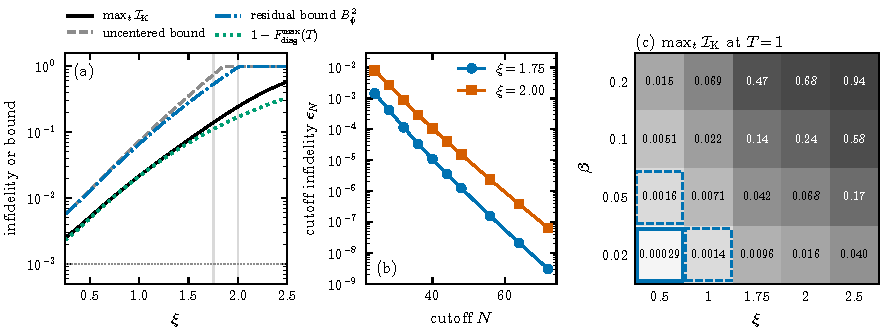
\includegraphics[width=\textwidth]{figures/fig_duffing_native.pdf}
\caption{Native Kerr evolution versus the Duffing target at \(\omega_0=1\) and \(T=1\). (a) Maximum infidelity of the native Kerr trajectory, the uncentered Duhamel bound of Eq.~\eqref{eq:df-bound}, the residual bound \(B_\psi^2\) of Theorem~\ref{thm:native-residual} (bounds capped at one), and the final-time floor \(1-F^{\max}_{\rm diag}(T)\) left by any number-diagonal control, as functions of the coherent amplitude at \(\beta=0.1\) and cutoff 80. Vertical lines mark the benchmark amplitudes and the dotted line \(10^{-3}\). (b) Convergence of the exact target trajectory with cutoff \(N\), measured by the maximum infidelity \(\epsilon_N\) against cutoff 80. (c) Maximum native-Kerr infidelity on the \((\beta,\xi)\) grid. A solid outline marks the point where Theorem~\ref{thm:native-residual} certifies native sufficiency at \(10^{-3}\), and dashed outlines the additional points certified at \(10^{-2}\). At \(\beta=0\) (not shown) native evolution is exact.}
\label{fig:df-diagnostics}
\end{figure*}

We set \(\omega_0=1\), which fixes the units of frequency and time. The corresponding bare harmonic period is \(2\pi/\omega_0\simeq6.28\). The initial states are real-displaced coherent states \(\ket{\xi}\), defined by \(\hat a\ket{\xi}=\xi\ket{\xi}\), with initial mean occupation
\(\langle\hat N\rangle_0=|\xi|^2 .\)
Coherent states provide a natural semiclassical probe of Duffing dynamics \cite{Dias_2006}. Increasing \(\xi\) also populates higher oscillator levels, where the number-changing matrix elements in Eq.~\eqref{eq:df-vcr} become larger.

We choose \(\beta=0.10\) as a representative benchmark and consider \(\xi=1.75\) and \(2.00\), corresponding to \(\langle\hat N\rangle_0=3.0625\) and \(4.00\), respectively. Each state is evolved over \(0\leq t\leq T\), with \(T=1.0\), or approximately \(0.16\) bare oscillation periods. These parameters are not presented as a universal threshold for breakdown of the rotating-wave approximation (RWA). Instead, the amplitude scan below directly establishes that the full Duffing and native Kerr trajectories are distinguishable over the selected interval.

For this benchmark, Eq.~\eqref{eq:df-fock-kerr} gives \(K_{\rm eff}=0.0375\). The analytic Kerr collapse estimates are \(t_{\rm c}=10.775\) for \(\xi=1.75\) and \(t_{\rm c}=9.428\) for \(\xi=2.00\). Thus \(T/t_{\rm c}=0.0928\) and \(0.1061\), respectively. These values are distinct from the threshold-based \(t_{\rm E}\) in Eq.~\eqref{eq:mean-field-validity-time}.

\paragraph{Trajectory-dependent action of the correction.}
To characterize the correction along the simulated trajectory, we define the shift-invariant ratio
\begin{align}
r_\psi(t)=\tfrac{\left\|\left[\lambda\hat V_{\rm cr}-\langle\lambda\hat V_{\rm cr}\rangle_{\psi_{\rm D}(t)}\right]\ket{\psi_{\rm D}(t)}\right\|}{\left\|\left[\hat H_{\rm D}-\langle\hat H_{\rm D}\rangle_{\psi_{\rm D}(t)}\right]\ket{\psi_{\rm D}(t)}\right\|}=\tfrac{\sigma_{\psi_{\rm D}(t)}(\lambda\hat V_{\rm cr})}{\sigma_{\psi_{\rm D}(t)}(\hat H_{\rm D})},
\label{eq:df-state-ratio}
\end{align}
where
\(\ket{\psi_{\rm D}(t)}=e^{-i\hat H_{\rm D}t}\ket{\xi}.\)
Subtracting the expectation values removes components that generate only an overall phase. Thus, \(r_\psi(t)\) measures the relative projective action of the correction on the state being evolved.

Using \(N=80\), we obtain $\max_{0\leq t\leq1}r_\psi(t)=0.600$ for $\xi=1.75$ and $\max_{0\leq t\leq1}r_\psi(t)=0.771$ for $\xi=2.00.$
Over the same interval, the maximum infidelity between the full Duffing and native Kerr trajectories,
\begin{align}
\mathcal I_{\rm K}(t)=1-\left|\braket{\psi_{\rm D}(t)}{\psi_{\rm K}(t)}\right|^2,\qquad\ket{\psi_{\rm K}(t)}=e^{-i\hat H_{\rm K}t}\ket{\xi},
\label{eq:df-native-infidelity}
\end{align}
is
\(\max_{0\leq t\leq1}\mathcal I_{\rm K}(t)=0.1388\) for $\xi=1.75$ and
$\max_{0\leq t\leq1}\mathcal I_{\rm K}(t)=0.2428$ for $\xi=2.00,$ evaluated on a 401-point grid. The target states at cutoffs 64 and 80 differ by at most \(1.5\times10^{-4}\) and \(6.2\times10^{-4}\) in projective distance at the two amplitudes [Fig.~\ref{fig:df-diagnostics}(b)].
These trajectory-resolved results, rather than the cutoff-space operator norms, establish that the number-changing remainder is dynamically important at the benchmark.

A complementary final-time diagnostic follows from the fact that a number-diagonal unitary can change only the phases of the initial Fock amplitudes. For each input separately, the largest fidelity attainable at time \(T\) by any number-diagonal unitary is therefore
\begin{align}
F_{\rm diag}^{\max}(T;\xi)=\left[\sum_n\left|\braket{n}{\psi_{\rm D}(T)}\right|\left|\braket{n}{\xi}\right|\right]^2 .
\label{eq:df-diagonal-ceiling}
\end{align}
This is an instance of the following statement, proved in Appendix~\ref{app:proofs}.

\begin{proposition}[Number-diagonal ceiling]
\label{prop:diagonal}
For normalized finite Fock states \(\psi\) and \(\varphi\), \(\max_{\Lambda}|\langle\varphi|\Lambda|\psi\rangle|^2=\bigl(\sum_n|\varphi_n||\psi_n|\bigr)^2\), where the maximum runs over number-diagonal unitaries \(\Lambda\) and is attained by \(\Lambda_{nn}=e^{i(\arg\varphi_n-\arg\psi_n)}\).
\end{proposition}

At \(T=1\), Eq.~\eqref{eq:df-diagonal-ceiling} gives \(0.8890\) for \(\xi=1.75\) and \(0.8309\) for \(\xi=2.00\). These are state-specific, final-time ceilings; they are not the fidelity of a single diagonal unitary optimized simultaneously for both inputs. Nevertheless, they show directly that a purely number-diagonal correction cannot reproduce the complete Duffing state at these benchmark points. The ceiling applies to any combination of Kerr waits and SNAP gates, since both are number diagonal, whereas displacement and squeezing change the number distribution and are not constrained by it.

\paragraph{Amplitude dependence and the Duhamel diagnostic.}
Within the finite Fock space, we suppress the superscript \((N)\) on the strict-cutoff operators and state vectors. For \(t\geq0\), Appendix~\ref{app:proofs} proves the phase-aligned Duhamel bound
\begin{align}
\left\|\ket{\psi_{\rm D}(t)}-e^{-iE_0t}\ket{\psi_{\rm K}(t)}\right\| &\leq |\lambda|\int_0^t\left\|\hat V_{\rm cr}\ket{\psi_{\rm K}(s)}\right\|\,{\rm d}s .
\label{eq:df-duhamel}
\end{align}
For normalized states, the global phase does not change the fidelity, and hence
\begin{align}
\mathcal I_{\rm K}(t) &\leq \lambda^2\left[\int_0^t\left\|\hat V_{\rm cr}e^{-i\hat H_{\rm K}s}\ket{\xi}\right\|\,{\rm d}s\right]^2 .
\label{eq:df-bound}
\end{align}
Because \(\hat H_{\rm K}\) is diagonal in the number basis, the integrand can be evaluated directly. Refining the quadrature grid from 401 to 801 points changes the integrals by less than \(2\times10^{-7}\).

At \(N=80\) and \(T=1\), the right-hand side of Eq.~\eqref{eq:df-bound} is \(0.7393\) for \(\xi=1.75\), compared with a direct maximum infidelity of \(0.1388\). For \(\xi=2.00\), the bound is \(1.4936\) and is therefore meaningless. The amplitude scan places the crossing of unity near \(\xi=1.86\), or \(\langle\hat N\rangle_0\simeq3.44\).

Over the sampled points with \(\langle\hat N\rangle_0>1\), log--log fits give the empirical relations
\begin{align}
\max_t\mathcal I_{\rm K}(t)\propto\langle\hat N\rangle_0^{1.89},\qquad\mathcal B_{\rm Duhamel}(T)\propto\langle\hat N\rangle_0^{2.43},
\end{align}
where \(\mathcal B_{\rm Duhamel}\) denotes the right-hand side of Eq.~\eqref{eq:df-bound}. These exponents describe only the finite parameter window sampled here and are not asymptotic scaling laws. Their difference explains why this particular norm-based estimate becomes rapidly uninformative. Theorem~\ref{thm:native-residual} removes the part of \(\lambda\hat V_{\rm cr}\) that acts as a phase on the Kerr trajectory. The resulting bound \(B_\psi(T)^2\) equals \(0.531\) at \(\xi=1.75\) and \(0.965\) at \(\xi=2.00\), crosses unity near \(\xi=2.01\), and grows as \(\langle\hat N\rangle_0^{2.10}\) over the same window [Fig.~\ref{fig:df-diagnostics}(a)]. It improves on Eq.~\eqref{eq:df-bound} but remains a sufficient condition, and we base the quantitative assessment at the benchmark amplitudes on the directly simulated trajectory infidelity.

Figure~\ref{fig:df-diagnostics}(c) extends the comparison to \(\beta\in\{0.02,0.05,0.1,0.2\}\) and \(\xi\in\{0.5,1,1.75,2,2.5\}\) at \(T=1\), with reference cutoffs 48, 64, and 80. At the threshold \(\mathcal I_\star=10^{-3}\), native Kerr evolution fails at 19 of these 20 points, and Theorem~\ref{thm:native-residual} certifies sufficiency at the remaining point, \(\beta=0.02\) and \(\xi=0.5\), where the maximum infidelity is \(2.9\times10^{-4}\). At \(\mathcal I_\star=10^{-2}\), the bound certifies three points, direct simulation shows failure at 14, and three points remain inconclusive. Wherever \(B_\psi^2<1\), the bound including its numerical margin exceeds the maximum infidelity by a factor between 1.8 and 4.2, so it certifies sufficiency when the actual error lies a few times below the threshold. At the three inconclusive points the simulated infidelities, \(5.1\times10^{-3}\), \(7.1\times10^{-3}\), and \(9.6\times10^{-3}\), lie below \(10^{-2}\), so native evolution does suffice there. The test leaves them open because it uses direct simulation only to establish failure, which keeps it applicable when the target cannot be simulated. At \(\beta=0\) the native and target Hamiltonians coincide, and all five points are sufficient. Over this window, less than a sixth of an oscillation period, the counter-rotating sector is therefore dynamically important at every tested point except the weakest nonlinearity with the smallest amplitude.

For a number-diagonal native Hamiltonian the uncentered bound of Eq.~\eqref{eq:df-duhamel} can also be evaluated without time evolution. Each monomial of \(\hat V_{\rm cr}\) shifts the photon number by a fixed amount, so its norm on \(e^{-i\hat H_{\rm K}s}\ket{\psi_0}\) depends only on the conserved number distribution. The triangle inequality applied to Eq.~\eqref{eq:df-duhamel} then gives
\begin{align}
\mathcal I_{\rm K}(t)\le\lambda^2t^2\Big[&\|\hat a^4\psi_0\|+\|\hat a^{\dagger4}\psi_0\|+4\|\hat a^{\dagger3}\hat a\psi_0\|\nonumber\\
&+4\|\hat a^\dagger\hat a^3\psi_0\|+6\|\hat a^2\psi_0\|+6\|\hat a^{\dagger2}\psi_0\|\Big]^2 ,
\label{eq:df-apriori}
\end{align}
which requires only the initial state and, by moment bounds on each term, is controlled by \(\langle\hat N^4\rangle_0\) and \(\langle\hat N^2\rangle_0\). On the grid of Fig.~\ref{fig:df-diagnostics}(c) this a priori bound certifies the same three points as \(B_\psi\) at \(10^{-2}\). At \(10^{-3}\) it gives \(1.1\times10^{-3}\) at \(\beta=0.02\), \(\xi=0.5\), just above the threshold.

Over this short window the first moments of the exact Duffing state stay within \(\varepsilon^\star_{\rm MF}=0.1\) of the classical Duffing trajectory at every grid point with \(\beta\le0.1\), with \(d_{\rm MF}(t)=\max\{|\langle\hat q\rangle-q_{\rm cl}|,|\langle\hat p\rangle-p_{\rm cl}|/\omega_0\}/\max\{1,|q(0)|,|p(0)|/\omega_0\}\). At \(\beta=0.2\) the threshold is crossed at \(t=0.62\) and \(0.40\) for \(\xi=0.5\) and 1. There the closure term \(-\beta[3\langle\hat q\rangle{\rm Var}(q)+\langle(\hat q-\langle\hat q\rangle)^3\rangle]\) in the momentum equation is comparable to or larger than the classical cubic force, because the zero-point variance is not small compared with \(\langle\hat q\rangle^2\). Over one bare period, \(T=2\pi\), the first moments at \(\beta=0.1\) cross the threshold at \(t=2.05\) and \(1.96\) for \(\xi=1.75\) and \(2.00\), and the native Kerr infidelity reaches \(0.650\) and \(0.852\). The compiled comparison below uses \(T=1\), inside the mean-field window.

\subsubsection{Compiling the counter-rotating sector}
\label{subsec:df-compile}

\begin{figure}[t]
\centering
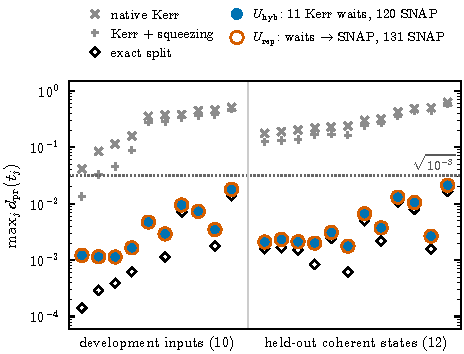
\includegraphics[width=\columnwidth]{figures/fig_duffing_correction.pdf}
\caption{Duffing correction at \(\beta=0.1\), \(T=1\), and \(r=10\) steps. Maximum projective distance from the cutoff-80 target over the grid \(t_j=jT/10\) for ten development inputs and twelve held-out coherent states, sorted by the native Kerr error within each group: native Kerr evolution, Kerr evolution with the exact squeezing correction, the exact symmetric split of Eq.~\eqref{eq:df-hybrid-step}, the compiled hybrid circuit \(U_{\rm hyb}\), and the circuit \(U_{\rm rep}\) in which all native waits are replaced by SNAP gates. The compiled circuits use padding cutoff 96. The dotted line is \(\sqrt{10^{-3}}\).}
\label{fig:df-correction}
\end{figure}

\begin{table}[t]
\caption{Resources and worst-case state error of the passing Duffing circuits (\(\beta=0.1\), \(T=1\), \(r=10\), \(L=12\)). Counts are ideal gates, with one SNAP phase vector per SNAP gate. The state error is the largest over the 22 inputs of the maximum distance plus the reference-cutoff, solver, and padding margins at padding cutoffs 96/112.}
\label{tab:duffing-resources}
\begin{ruledtabular}
\begin{tabular}{lccccc}
Circuit & SNAP & Displ. & Squeezing & Kerr waits & State error \\
\hline
\(U_{\rm hyb}\) & 120 & 120 & 20 & 11 & 0.0234 \\
\(U_{\rm rep}\) & 131 & 120 & 20 & 0 & 0.0235 \\
\end{tabular}
\end{ruledtabular}
\end{table}

Beyond the RWA, the correction can be separated into Gaussian and non-Gaussian parts,
\begin{align}
\hat V_{\rm cr}&=\hat V_2+\hat V_4,\qquad\hat V_2=6(\hat a^2+\hat a^{\dagger2}),\nonumber\\
\hat V_4&=\hat a^{\dagger4}+4\hat a^{\dagger3}\hat a+\hat a^4+4\hat a^\dagger\hat a^3 .
\label{eq:df-v2-v4}
\end{align}
The quadratic contribution is implemented exactly, within the chosen truncation, as a squeezing operation,
\begin{align}
e^{-i\lambda\hat V_2\Delta t}=S(\zeta),\qquad S(\zeta)&=\exp\left[\tfrac{1}{2}\left(\zeta^*\hat a^2-\zeta\hat a^{\dagger2}\right)\right],\nonumber\\
\zeta&=12i\lambda\Delta t.
\label{eq:df-squeezing}
\end{align}
The residual quartic operator \(\hat V_4\) is non-Gaussian and number-changing and must therefore be synthesized with programmable non-Gaussian gates.

\paragraph{SNAP-plus-displacement ansatz.}
We approximate the non-Gaussian short-time block $U_{4,\rm target} = e^{-i\lambda\hat V_4\Delta t}$ with the SNAP-plus-displacement (SNAP+D) decomposition \cite{Krastanov_2015,Fosel2020SNAP,Kudra2022SNAPD}
\begin{align}
U_{\rm comp}&=\prod_{\ell=1}^{L}D(\alpha_\ell)\,S_d(\boldsymbol\theta_\ell),\nonumber\\
S_d(\boldsymbol\theta)&=\sum_{n<d}e^{i\theta_n}\ketbra{n}{n}+(I-P_d),
\label{eq:snapd-ansatz}
\end{align}
where \(D(\alpha)=\exp(\alpha\hat a^\dagger-\alpha^*\hat a)\) and \(P_d\) projects onto the first \(d\) levels, in a padded circuit space of dimension \(D_{\rm pad}\). The distinction between \(d\) and \(D_{\rm pad}\) is essential. Displacements can populate levels above the active SNAP space even though the SNAP phases act only on the first \(d\) number states. The compiled circuit must therefore be simulated in a larger padded space, and both population above \(d\) and population near the padded boundary must be checked explicitly.

The native Kerr evolution, analytic squeezing, and compiled quartic block are combined using the symmetric step \cite{Strang1968}
\begin{align}
U_{\rm hyb}(\Delta t) ={}& e^{-iE_0\Delta t}e^{-i\hat H_{\rm K}\Delta t/2}e^{-i\lambda\hat V_2\Delta t/2}\nonumber\\
&\quad U_{\rm comp}\,e^{-i\lambda\hat V_2\Delta t/2}e^{-i\hat H_{\rm K}\Delta t/2}.
\label{eq:df-hybrid-step}
\end{align}
The scalar prefactor restores the evolution generated by the full \(\hat H_{\rm D}\).
Replacing \(U_{\rm comp}\) by the exact block \(U_{4,\rm target}\) defines the exact symmetric split, which isolates the product-formula error at the selected time step. The additional difference produced by replacing \(U_{4,\rm target}\) with \(U_{\rm comp}\) measures the effect of compilation.

\paragraph{Training and evaluation.}
Equation~\eqref{eq:action-sum} requires the compiled block to act correctly on the states that enter it along the exact target trajectory. We therefore fit \(U_{\rm comp}\) to the exact action of \(U_{4,\rm target}\) on the states \(U^k\psi_a\), \(k=0,\ldots,r-1\), after the preceding Kerr and squeezing half steps, where \(U\) is the exact Duffing step and \(\psi_a\) runs over 24 coherent initial states with amplitudes \(\rho e^{im\pi/4}\), \(\rho\in\{1,1.5,2.25\}\), and \(m=0,\ldots,7\). The objective is the Frobenius distance between the compiled and target columns with one common phase, plus a small displacement penalty (Appendix~\ref{app:numerics}). We use \(\beta=0.1\), \(T=1\), \(r=10\) steps, \(L=12\) layers, \(d=48\), \(D_{\rm pad}=96\), and reference cutoff 80. The selected circuit is evaluated on 22 inputs outside the training set. Ten development inputs, used to diagnose the real-amplitude training set of Appendix~\ref{app:duffing-training}, are the coherent states with amplitudes \(1.75\) and 2 and phases 0, \(\pi/4\), and \(\pi/2\), together with \(\ket0\), \(\ket1\), \((\ket0+\ket1)/\sqrt2\), and \((\ket0+i\ket2)/\sqrt2\). Twelve held-out coherent states have amplitudes and phases drawn at random before training. Their amplitudes, from 1.13 to 2.10, lie inside the training range, so extrapolation to larger amplitudes is not tested.

\paragraph{Results.}
Figure~\ref{fig:df-correction} compares five constructions on the grid \(t_j=jT/10\). Native Kerr evolution reaches projective distances up to 0.62 from the target, and adding the exact Gaussian correction lowers them only to 0.58. The number-changing quartic term \(\hat V_4\) therefore carries most of the correction, as Proposition~\ref{prop:diagonal} anticipates for number-diagonal controls. The exact symmetric split stays within 0.017 of the target, and the compiled hybrid circuit exceeds it by at most \(5\times10^{-3}\) on every input. Its largest distance is 0.021 on the held-out inputs and 0.018 on the development inputs. Including the reference-cutoff, solver, and padding margins, the largest state error is \(0.0234\), below \(\sqrt{10^{-3}}\approx0.0316\), and the same gate parameters give 0.0222 at padding cutoffs 128 and 160, with boundary populations below \(10^{-9}\). The composition bound of Eq.~\eqref{eq:action-sum} reaches 0.053 on one held-out input, above \(\sqrt{10^{-3}}\), so the accuracy of this circuit rests on direct simulation. A circuit trained only on real coherent amplitudes reproduces the two real benchmark states but reaches distances above 0.85 on rotated inputs (Appendix~\ref{app:duffing-training}), because the states entering the quartic block then leave the region of phase space covered by training.

\paragraph{Replacing native Kerr waits by SNAP gates.}
Every native wait \(K(\tau)=e^{-i\tau\hat H_{\rm K}}\) in the circuit \(U_{\rm hyb}^r\) is number diagonal. After adjacent half waits are merged, \(r+1\) waits remain, and each can be replaced by the SNAP gate
\begin{align}
\widetilde K_d(\tau)=\sum_{n<d}e^{-i\tau(\omega_{\rm eff}n+K_{\rm eff}n^2)}\ketbra{n}{n}+(I-P_d),
\label{eq:kerr-snap}
\end{align}
whose phases follow from \(\hat H_{\rm K}\) without optimization. The two operators agree on the first \(d\) levels and are unitary, so \(\|(\widetilde K_d-K)\chi\|\le2\|(I-P_d)\chi\|\), and telescoping over the replaced gates gives
\begin{align}
\big\|(U_{\rm rep}-U_{\rm hyb}^r)\psi\big\|\le2\sum_{j=1}^{r+1}\big\|(I-P_d)\chi_j\big\| ,
\label{eq:kerr-tail}
\end{align}
where \(U_{\rm rep}\) is the circuit with all waits replaced and \(\chi_j\) is the state of \(U_{\rm hyb}^r\psi\) just before the \(j\)th wait (Appendix~\ref{app:proofs}). The replaced circuit uses 131 SNAP gates in place of 120 SNAP gates and 11 native waits, with the same displacements and squeezing pulses (Table~\ref{tab:duffing-resources}). Its distances coincide with those of \(U_{\rm hyb}\) to within \(2.1\times10^{-5}\) on all 22 inputs (Fig.~\ref{fig:df-correction}), and its largest state error is \(0.0235\). The tail bound of Eq.~\eqref{eq:kerr-tail} reaches 0.021 for the most populated input, so the agreement of the two circuits is established by direct simulation rather than by the bound. The two circuits share the optimized block \(U_{\rm comp}\), and the replacement phases need no optimization, so the replacement adds no compilation cost either. In the ideal gate model the native Kerr interaction therefore saves 11 of 131 SNAP gates, or 11 of 271 programmable primitives, and its remaining value lies in the duration of those gates relative to the native waits (Sec.~\ref{subsec:duration}).


\subsection{Deformed (double) sine-Gordon lattice}
\label{sec:dsg}

\begin{figure*}[t]
\centering
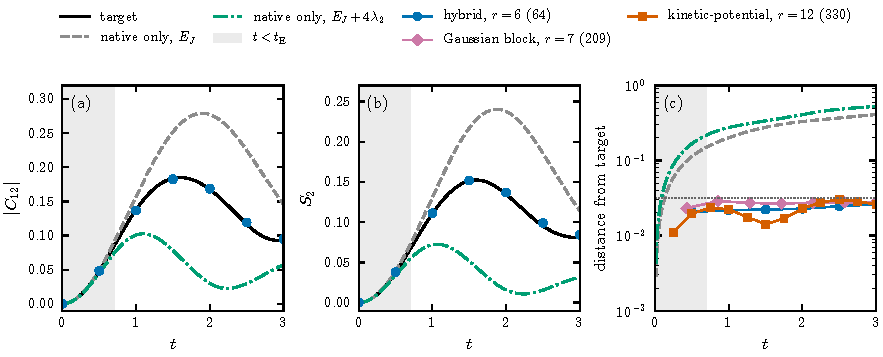
\includegraphics[width=\textwidth]{figures/fig_dsg_dynamics.pdf}
\caption{Two-site double sine-Gordon lattice at \(E_J=1\), \(\lambda_2=0.3\), \(\kappa=1\), with the product coherent preparation \(\langle\hat\phi\rangle=(1,0)\), \(\omega_b=\sqrt3\), and local cutoff 128. (a) Modulus of the connected vertex correlation, (b) second R\'enyi entropy of one site, and (c) distance from the target state, projective for native-only evolution with the original and the retuned onsite energy and Bures for the reduced state of the cheapest hybrid, Gaussian-block, and kinetic--potential circuits of Table~\ref{tab:dsg-resources} at \(\lambda_2=0.3\), labeled by \(r\) and primitive count. Circuit values are shown at the outer-step times, and the circles in (a) and (b) are the hybrid circuit. Shading marks the window \(t<t_{\rm E}\) in which the first moments follow the classical field, and the dotted line in (c) is \(\sqrt{10^{-3}}\).}
\label{fig:dsg-dynamics}
\end{figure*}

Adding a second harmonic to the onsite potential of Eq.~\eqref{eq:sg-lattice} gives the deformed, or double, sine-Gordon lattice,
\begin{align}
H_{\rm target}=H_{\rm SG}+\lambda_2\sum_j\bigl[1-\cos(2\phi_j)\bigr].
\label{eq:dsg-target}
\end{align}
The double sine-Gordon model is a nonintegrable deformation of the sine-Gordon model \cite{Delfino1998DSG}. A Josephson array that includes \(0\)--\(\pi\) circuits realizes such a second cosine and has been proposed to study soliton confinement \cite{RoyLukyanov2023Confinement,Roy2023Multicritical}, and circuit elements dominated by \(\cos2\phi\) have been designed and measured \cite{Smith2020cos2phi,Larsen2020Parity}. Here the second harmonic is the correction to a native sine-Gordon lattice, \(H_{\rm native}=H_{\rm SG}\) and \(\Delta H=\lambda_2\sum_j(1-\cos2\phi_j)\). Its centered norm approaches \(2\lambda_2\) as the phase resolution grows, so \(T\|\Delta H_\circ\|_2\) exceeds \(\epsilon^\star_{\rm traj}/3\) by two orders of magnitude and the target is Class II--U. The ratio \(\eta_H\) falls from 0.027 to 0.008 between local cutoffs 16 and 48 and keeps falling at larger cutoffs, because the kinetic energy increases the target norm (Appendix~\ref{app:class-diagnostics}).

We study two sites with open boundaries, \(\kappa=1\), \(E_J=1\), and \(\lambda_2=0.3\), with \(\cos(m\hat\phi_j)\) and \(\hat\Pi_j^2\) defined as functions of the truncated quadratures (Appendix~\ref{app:numerics}). The initial state is the product coherent state with \(\langle\hat\phi\rangle=(1,0)\), \(\langle\hat\Pi\rangle=(0,0)\), and \(\omega_b=\sqrt3\), and we evolve to \(T=5.2/\sqrt3\approx3.00\), as in the \(E_J=1\) calibration of Sec.~\ref{subsec:sg-classical}. At local cutoff 128 the target state differs from the cutoff-96 state by at most \(1.31\times10^{-3}\) in projective distance, and an independent adaptive integration agrees to \(3\times10^{-9}\) (Appendix~\ref{app:dsg-convergence}).

Besides the original native lattice, we consider a retuned native lattice based on the exact identity
\begin{align}
&E_J(1-\cos\phi)+\lambda_2(1-\cos2\phi)\nonumber\\
&\quad=(E_J+4\lambda_2)(1-\cos\phi)-2\lambda_2(1-\cos\phi)^2 .
\label{eq:retuning}
\end{align}
With \(E_J'=E_J+4\lambda_2=2.2\), the retuned native Hamiltonian matches the curvature of the target potential at \(\phi=0\) and leaves the correction \(-2\lambda_2\sum_j(1-\cos\phi_j)^2\), which is quartic in \(\phi_j\) at small amplitude. The retuning keeps the basis, the initial state, and the horizon unchanged, and it assumes that the onsite Josephson energy can be tuned independently of the kinetic and bond terms.

We compare two quantum observables that the classical field does not contain, the connected vertex correlation
\begin{align}
C_{12}=\langle e^{i\hat\phi_1}e^{-i\hat\phi_2}\rangle-\langle e^{i\hat\phi_1}\rangle\langle e^{-i\hat\phi_2}\rangle
\end{align}
and the second R\'enyi entropy \(S_2=-\log{\rm Tr}\,\rho_1^2\) of the reduced state \(\rho_1\) of site 1, which quantifies the entanglement between the two sites when the two-site state is pure.

\subsubsection{Native-only evolution and quantum observables}

Figure~\ref{fig:dsg-dynamics} shows that omitting the correction changes both observables by amounts comparable to their magnitudes. In the target evolution \(|C_{12}|\) peaks at 0.185 and \(S_2\) at 0.152. The original native lattice overestimates both, with maximum deviations of 0.115 in \(C_{12}\) and 0.105 in \(S_2\), and the retuned lattice underestimates them, with deviations of 0.138 and 0.121. These differences exceed the numerical uncertainty of \(C_{12}\), below \(2\times10^{-6}\), by more than four orders of magnitude. Both observables decrease as the onsite curvature \(V''(\phi_j)\), averaged over each trajectory and both sites, increases from 0.66 for the original native lattice to 1.02 for the target and 1.63 for the retuned lattice. This is consistent with a stiffer onsite potential weakening the relative effect of the bond coupling, although three trajectories do not establish that mechanism. The curvatures are not ordered at every phase. The difference \(V_{\rm target}''-V_{\rm native}''=4\lambda_2\cos2\phi\) changes sign at \(|\phi|=\pi/4\), and its expectation for site 1 is negative in the initial state, so Eq.~\eqref{eq:retuning} alone does not order the observables. The state distances from the target reach 0.411 and 0.528, so curvature matching does not reduce the error on this preparation.

With \(d_{\rm MF}\) defined as in Sec.~\ref{subsec:sg-classical} against the classical double sine-Gordon lattice, the first moments cross \(\varepsilon^\star_{\rm MF}=0.1\) at \(t_{\rm E}=0.703\), within the grid bracket \([0.692,0.704]\) and before a quarter of the window. The correlation and entanglement differences that follow therefore arise in the regime where the classical field no longer describes the dynamics. Reproducing them requires simulating the quantum target, which is still classically tractable at two sites (Sec.~\ref{subsec:hardware}).

\subsubsection{Hybrid versus programmable circuits}

\begin{figure*}[t]
\centering
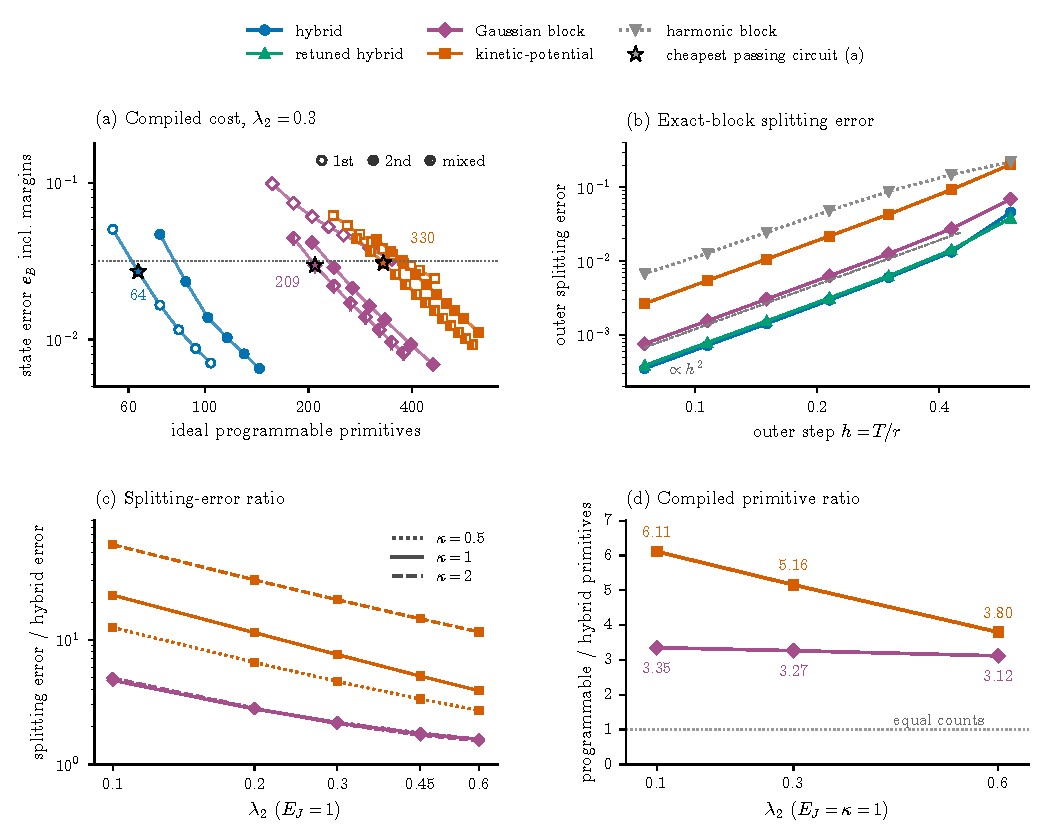
\includegraphics[width=\textwidth]{figures/fig_dsg_resources.pdf}
\caption{Hybrid and programmable circuits for the double sine-Gordon instance of Fig.~\ref{fig:dsg-dynamics}. (a) State error including numerical margins at cutoffs 128/160 against the number of ideal programmable primitives at \(\lambda_2=0.3\), with \(s=1\) and the number \(r\) of outer steps varying along each line. Open and filled symbols use first- and second-order blocks for every harmonic, and half-filled symbols second-order blocks for the Josephson harmonic and first-order blocks for the \(\lambda_2\) harmonic. The dotted line is \(\sqrt{10^{-3}}\), and stars mark the cheapest circuit of each route that meets all criteria, labeled by its primitive count. (b) Outer splitting error with exact blocks at local cutoff 80, maximized over the outer-step times, against the outer step \(h=T/r\) for the hybrid split \(H_{\rm SG}|\Delta H\), the retuned hybrid split, the Gaussian-block split \((H_{\rm kin}+H_{\rm bond})|(V_J+\Delta H)\), the kinetic--potential split \(H_{\rm kin}|(H_{\rm bond}+V_J+\Delta H)\), and the harmonic-block split, which also moves the harmonic part of the onsite potential into the Gaussian block. The dashed guide is proportional to \(h^2\). (c) Lines: splitting errors of the Gaussian-block and kinetic--potential formulas relative to the hybrid one at \(r=20\) and local cutoff 64, as functions of \(\lambda_2\) for \(E_J=1\) and \(\kappa=0.5\), 1, and 2. Stars: primitive counts of the cheapest compiled programmable circuits relative to the cheapest hybrid circuit at \(\kappa=1\) (Table~\ref{tab:dsg-resources}).}
\label{fig:dsg-resources}
\end{figure*}

\begin{table*}[t]
\caption{Cheapest double sine-Gordon circuit of each route that meets all numerical criteria at cutoffs 128/160 (\(E_J=1\), \(\kappa=1\), one ancillary qubit, \(s=1\)). The circuit marked \(\ast\) exceeds the boundary limit only at padding 128 and is evaluated at cutoffs 160/192, where it meets every criterion. At cutoffs 128/160 the cheapest Gaussian-block circuit at \(\lambda_2=0.6\) has second-order blocks, \(r=9\), and 301 primitives. The last four rows are for three sites, where the hybrid circuit is also listed with one more outer step, and the others are for two sites. Orders give the block order of the Josephson and \(\lambda_2\) harmonics. Counts are ideal primitives after exact merging: qubit-controlled displacements (CD), qubit rotations about \(y\) and \(z\), and Gaussian quadratic gates. The two \(R_z\) rotations belong to the qubit basis change applied once per circuit. The state error \(e_B\) and the observable errors \(e_C\) and \(e_S\) include numerical margins. Preparation, readout, and physical pulse durations are additional resources.}
\label{tab:dsg-resources}
\begin{ruledtabular}
\begin{tabular}{llcccccccccc}
\(\lambda_2\) & Circuit & \(r\) & Orders & CD & \(R_y\) & \(R_z\) & Gaussian & Total & Native waits & \(e_B\) & \(e_C\), \(e_S\) \\
\hline
0.1 & Hybrid & 5 & --/1 & 30 & 22 & 2 & 0 & 54 & 6 & 0.0141 & 0.0008, 0.0010 \\
  & Gaussian block & 6 & 2/1 & 72 & 62 & 2 & 45 & 181 & 0 & 0.0280 & 0.0066, 0.0055 \\
  & Kinetic--potential & 12 & 2/1 & 144 & 122 & 2 & 62 & 330 & 0 & 0.0291 & 0.0081, 0.0074 \\
0.3 & Hybrid & 6 & --/1 & 36 & 26 & 2 & 0 & 64 & 7 & 0.0271 & 0.0028, 0.0037 \\
  & Gaussian block & 7 & 2/1 & 84 & 72 & 2 & 51 & 209 & 0 & 0.0298 & 0.0047, 0.0071 \\
  & Kinetic--potential & 12 & 2/1 & 144 & 122 & 2 & 62 & 330 & 0 & 0.0307 & 0.0088, 0.0077 \\
0.6 & Hybrid & 9 & --/1 & 54 & 38 & 2 & 0 & 94 & 10 & 0.0272 & 0.0042, 0.0049 \\
  & Gaussian block\(^\ast\) & 10 & 2/1 & 120 & 102 & 2 & 69 & 293 & 0 & 0.0247 & 0.0061, 0.0078 \\
  & Kinetic--potential & 13 & 2/1 & 156 & 132 & 2 & 67 & 357 & 0 & 0.0302 & 0.0086, 0.0093 \\
\hline
0.3 & Hybrid & 6 & --/1 & 54 & 38 & 2 & 0 & 94 & 7 & 0.0315 & 0.0026, 0.0032 \\
  & Hybrid & 7 & --/1 & 63 & 44 & 2 & 0 & 109 & 8 & 0.0187 & 0.0017, 0.0021 \\
  & Gaussian block & 8 & 2/1 & 144 & 122 & 2 & 114 & 382 & 0 & 0.0262 & 0.0026, 0.0026 \\
  & Kinetic--potential & 13 & 2/1 & 234 & 197 & 2 & 107 & 540 & 0 & 0.0303 & 0.0050, 0.0056 \\
\end{tabular}
\end{ruledtabular}
\end{table*}

We compare the circuits on the same finite model and initial state. We write \(H_{\rm SG}=H_{\rm kin}+H_{\rm bond}+V_J\), with the kinetic energy \(H_{\rm kin}=\sum_j\hat\Pi_j^2/2\), the bond \(H_{\rm bond}=\tfrac{\kappa}{2}(\hat\phi_1-\hat\phi_2)^2\), and the Josephson potential \(V_J=E_J\sum_j(1-\cos\hat\phi_j)\), and we denote by \(A|B\) the symmetric product formula \(e^{-ihA/2}e^{-ihB}e^{-ihA/2}\) with outer step \(h=T/r\). The hybrid circuit implements \(H_{\rm SG}|\Delta H\),
\begin{align}
W_{\rm hyb}=e^{-i\frac h2H_{\rm SG}}\,C_{\lambda_2}(h)\,e^{-i\frac h2H_{\rm SG}},
\end{align}
where \(C_{\lambda_2}(h)\) implements \(e^{-ih\lambda_2\sum_j(1-\cos2\hat\phi_j)}\) with the trigonometric continuous-variable gates of Ref.~\cite{Rainaldi2026TrigonometricCV}. The construction uses a single ancillary qubit, reused coherently for every site and harmonic, together with qubit-controlled displacements and qubit rotations, and each harmonic block has \(s\) internal subdivisions with first- or second-order internal splitting. The qubit basis change that the construction requires is applied once at the start and once at the end of a circuit, so each elementary factor needs two controlled displacements and one rotation (Appendix~\ref{app:trig}). The retuned hybrid circuit replaces the native half steps by retuned ones and compiles the two-harmonic correction of Eq.~\eqref{eq:retuning}. Two programmable circuits use no native evolution and implement both harmonics with the same trigonometric gates. The kinetic--potential circuit implements \(H_{\rm kin}|(H_{\rm bond}+V_J+\Delta H)\), with the kinetic and bond terms as Gaussian gates. The Gaussian-block circuit implements \((H_{\rm kin}+H_{\rm bond})|(V_J+\Delta H)\). Its quadratic part generates a two-mode Gaussian unitary, which the circuit applies as a quadratic gate in the momenta \(\hat\Pi_j\) between two quadratic gates in the phases \(\hat\phi_j\). This factorization is exact for canonical operators, and at finite cutoff it differs from the truncated Gaussian block by less than \(10^{-3}\) on the states that enter it, a difference included in the circuit errors below (Appendix~\ref{app:trig}). The SNAP+D hybrid circuit compiles the local correction into SNAP+D layers by numerical optimization. We count ideal programmable primitives after exact merging of adjacent rotations and Gaussian factors, and we count native waits separately. Each circuit uses \(s=1\). Its harmonic blocks are all first order, all second order, or, for the programmable circuits, second order for the Josephson harmonic and first order for the \(\lambda_2\) harmonic, and a circuit is accepted when it meets all criteria at cutoffs 128/160. The state error is the Bures distance of the reduced system state from the target, maximized over the outer-step times, plus the reference-cutoff, solver, and padding margins. The observable errors of \(C_{12}\) and \(S_2\) and the population of the four highest levels of either mode, which must stay below \(10^{-6}\), are checked separately (Appendix~\ref{app:numerics}).

Figure~\ref{fig:dsg-resources}(a) shows the state error against the primitive count as the number \(r\) of outer steps is scanned, and Table~\ref{tab:dsg-resources} lists the cheapest circuit of each route that meets all criteria. At \(\lambda_2=0.3\) the hybrid circuit needs 64 primitives and 7 native waits (\(r=6\), first-order blocks), the Gaussian-block circuit 209 primitives (\(r=7\)), and the kinetic--potential circuit 330 (\(r=12\)). Both programmable circuits are cheapest with a second-order block for the Josephson harmonic, whose coefficient is \(E_J=1\), and a first-order block for the \(\lambda_2\) harmonic. Under a common accuracy criterion, native evolution therefore reduces the programmable primitive count by a factor of 3.3 relative to the Gaussian-block circuit and 5.2 relative to the kinetic--potential circuit, and it reduces the number of controlled displacements, the entangling operations of the trigonometric gates, by factors of 2.3 and 4.0. At equal step count the Gaussian-block circuit needs 2.8 times the primitives of the hybrid circuit, 209 against 74 at \(r=7\), because it compiles two harmonics per site and adds Gaussian gates. The remaining factor of 1.2 comes from the coarser step that the hybrid circuit tolerates. Lowering the infidelity threshold from \(10^{-3}\) to \(10^{-4}\), with the other criteria unchanged, raises the saving relative to the Gaussian-block circuit to 3.7, because the hybrid circuit then needs 9 outer steps and the Gaussian-block circuit 12. The acceptance rule maximizes each error over the outer-step times of the circuit, so circuits with different \(r\) are checked at different times. At the common readout times \(t_k=kT/20\), each reached by its own circuit of \(\lceil t_k/h\rceil\) equal steps, the three cheapest circuits still pass and every cheaper circuit still fails (Appendix~\ref{app:dsg-convergence}). Without changing any parameter, the three cheapest circuits also meet every criterion on a second coherent preparation with \(\langle\hat\phi\rangle=(0.75,0)\) and \(\langle\hat\Pi\rangle=(0.25,0)\), with state errors 0.0256, 0.0288, and 0.0284. Restricted to \(r=10\) and 20, the cheapest circuits that pass at cutoffs 128/160 have 104 primitives for the hybrid route and 466 for the kinetic--potential route, and in the same comparison at cutoffs 96/128 internal subdivisions up to \(s=32\) lower neither count (Appendix~\ref{app:trig}). The retuned hybrid circuit was evaluated only in that comparison, where it passes with second-order blocks at \(r=10\) and 264 primitives, against 144 for the hybrid circuit with the same blocks and step count, because its correction contains two harmonics.

Figure~\ref{fig:dsg-resources}(b) separates the outer splitting error from the compilation error. With exact blocks at local cutoff 80, the splitting errors of the hybrid, retuned, Gaussian-block, and kinetic--potential formulas scale approximately as \(h^2\) for \(r\ge7\). The hybrid circuit splits the native Hamiltonian from the correction, so its leading error terms are nested commutators that contain \(\Delta H\) at least once \cite{Childs2021Trotter}, and its splitting error is approximately proportional to \(\lambda_2\). The kinetic--potential formula has 7.1 times the hybrid splitting error at \(r=10\) and 7.5 times at \(r=20\), but most of this factor comes from splitting the kinetic energy from the bond, since the Gaussian-block formula has 2.1 to 2.2 times the hybrid error for \(r\ge7\). A harmonic-block formula that also moves the harmonic part of the onsite potential into the Gaussian block has a larger error, because the anharmonic remainder is not small at the phase amplitudes reached here. Figure~\ref{fig:dsg-resources}(c) repeats the comparison for \(\lambda_2\) from 0.1 to 0.6 and \(\kappa\) from 0.5 to 2 at \(E_J=1\), with the preparation, basis, and horizon unchanged. At \(r=20\) the Gaussian-block formula has 4.7 to 4.9 times the hybrid splitting error at \(\lambda_2=0.1\) and 1.55 to 1.59 times at 0.6, nearly independent of \(\kappa\), whereas the ratio for the kinetic--potential formula grows with \(\kappa\), from 2.7 at \(\kappa=0.5\) and \(\lambda_2=0.6\) to about 58 at \(\kappa=2\) and \(\lambda_2=0.1\).

The compiled circuits depend much less on \(\lambda_2\) than the splitting errors do (Table~\ref{tab:dsg-resources}). The hybrid circuit needs 54 primitives at \(\lambda_2=0.1\) and 94 at 0.6, and its saving relative to the Gaussian-block circuit is 3.4 and 3.1, whereas the saving relative to the kinetic--potential circuit falls from 6.1 to 3.8. At \(\lambda_2=0.6\) the Gaussian-block circuits with mixed block orders and \(r=10\) to 12 exceed the boundary limit at padding 128, although not at 160, and at cutoffs 160/192 they meet every criterion. We therefore list the one with \(r=10\) and 293 primitives. The rule at cutoffs 128/160 alone would select a circuit with 301 primitives and give a saving of 3.2. At equal step count the per-step cost of the programmable circuits, which compile the Josephson harmonic and apply Gaussian gates in every step, accounts for a factor of 2.8 at all three values of \(\lambda_2\). The cheapest hybrid circuit uses at most one outer step fewer than the cheapest Gaussian-block circuit, so the larger splitting advantage at small \(\lambda_2\) has little effect on the count. All nine cheapest circuits meet every criterion on the second preparation. The splitting advantage matters at tighter thresholds. At \(\mathcal I_\star=10^{-4}\) the saving relative to the Gaussian-block circuit is 4.6, 3.7, and 2.7 at \(\lambda_2=0.1\), 0.3, and 0.6 (Appendix~\ref{app:dsg-convergence}). It grows where the hybrid splitting error is several times smaller than the programmable one and falls at \(\lambda_2=0.6\), where the two splitting errors differ by a factor of 1.6 and the cheapest hybrid circuit needs second-order blocks.

On an open chain of three sites with the same parameters and the preparation \(\langle\hat\phi\rangle=(1,0,0)\), the Gaussian-block and kinetic--potential routes need 382 and 540 primitives at cutoffs 128/160 (\(r=8\) and 13), and the hybrid route with \(r=7\) needs 109 primitives and has a state error of 0.0187 (Table~\ref{tab:dsg-resources}). The savings, 3.5 and 5.0, are close to the two-site values, and the controlled displacements are reduced by factors of 2.3 and 3.7. The cheapest passing hybrid circuit has \(r=6\) and 94 primitives, but its state error of 0.0315 lies just below \(\sqrt{10^{-3}}\approx0.0316\), so the larger savings it gives, 4.1 and 5.7, depend on where the threshold falls between two step numbers. The three-site target is more compact in the Fock basis than the two-site one. Its population with some mode above level 60 stays below \(9\times10^{-8}\), whereas on two sites it reaches \(4\times10^{-5}\), and the three-site target changes by \(1.7\times10^{-6}\) between local cutoffs 128 and 160 (Appendix~\ref{app:numerics}). We did not evaluate the second preparation or the common readout times of Appendix~\ref{app:dsg-convergence} on three sites.

The SNAP+D correction does not reach the threshold. The six circuits selected from zero-displacement starts have state errors between 0.103 and 0.144, and starts that break the displacement symmetry, a larger training space, and longer optimization lower the best error only to 0.057 (Appendix~\ref{app:dsg-snap}). The local target and the Fock-state training inputs are closed under parity, which makes the training objective even in the displacements, so vanishing displacements are a stationary point. Many runs converge to nearly number-diagonal circuits, which cannot reproduce the correction by Proposition~\ref{prop:diagonal}. The trigonometric construction avoids this difficulty because it implements each harmonic analytically.

In the frame of the elementary factors, which differs from that of the compiled pulses by the qubit basis change (Appendix~\ref{app:trig}), the ancillary qubit returns close to \(\ket0\) after every potential block. For every circuit of Table~\ref{tab:dsg-resources} its excited population at the outer-step times stays below \(5\times10^{-4}\), and for the nine two-site circuits the loss of system purity stays below \(10^{-3}\), which enters the state error through the Bures distance. Because the system state of a compiled circuit is then slightly mixed, its value of \(S_2\) also contains the residual correlation with the qubit, and we use it as an observable to be reproduced without reading it as intersite entanglement. For the hybrid circuit with second-order blocks, the composition bound of Eq.~\eqref{eq:action-sum} equals 0.051 at \(r=10\), above \(\sqrt{10^{-3}}\), although the simulated error is 0.0065, and 0.013 at \(r=20\), so it is sufficient but not tight at coarse steps.


\section{Discussion}
\label{sec:discussion}

\subsection{What a native interaction is worth}
\label{subsec:worth}

The three benchmarks separate two questions that a class label alone does not answer. Whether a correction is needed depends on the input states and the time window, and Theorem~\ref{thm:native-residual} together with direct simulation answers it for specified inputs. How much a native interaction saves depends on how cheaply the same evolution can be emulated with the available programmable primitives. The Kerr interaction belongs to the number-operator dictionary \(\mathcal D_J^{N}\), whose elements a SNAP gate reproduces exactly on a finite set of levels, so replacing the 11 native Kerr waits of the Duffing circuit by SNAP gates adds 11 gates to 120 and changes neither the accuracy nor the other gates. The Josephson cosine belongs to the trigonometric dictionary and does not commute with the kinetic energy. Its programmable emulation needs trigonometric gates with an ancillary qubit and a product formula that separates it from the kinetic energy. Native evolution removes both costs for the Josephson harmonic and leaves only the correction to be compiled and split. In the double sine-Gordon instance the hybrid circuit meets the accuracy criterion with 3.1 to 3.4 times fewer primitives than the best programmable circuit tested at the three tested values of \(\lambda_2\), and with 3.8 to 6.1 times fewer than a kinetic--potential circuit. Most of the first factor comes from compiling the Josephson harmonic in every programmable step, so it depends little on the size of the correction. The rest depends on how the splitting errors compare, and over infidelity thresholds up to ten times stricter the factor stays between 2.6 and 4.6. On three sites the factor is 3.5 for the hybrid circuit with seven outer steps and 4.1 for the cheapest passing one, whose error lies at the threshold, and two lattice sizes do not establish a dependence on size. The counts also leave out classical compilation, which is the same for the two Duffing circuits and absent for the analytic trigonometric gates, and the physical duration discussed in Sec.~\ref{subsec:duration}. In these two examples native implementation pays when the interaction is not diagonal in the basis of a cheap programmable phase gate and does not commute with the rest of the Hamiltonian.

Native retuning is not a substitute for a correction in the double sine-Gordon example. Matching the curvature of the double sine-Gordon potential leaves a correction that is small near \(\phi=0\) but not at the prepared amplitude, and it increases both the state error and the observable errors of native-only evolution. A retuned native lattice with a compiled correction does meet the accuracy target, but its correction contains two harmonics and costs 264 primitives with second-order blocks at \(r=10\), against 144 for the hybrid circuit with the same blocks and step count.

\subsection{Physical duration}
\label{subsec:duration}

Primitive counts do not order physical durations, because a native wait has zero programmable cost but a finite duration. For the Duffing pair of Table~\ref{tab:duffing-resources}, with identical displacement and squeezing schedules and no overlap between pulses and waits, the durations are
\begin{align}
t_{U_{\rm hyb}}&=t_{\rm common}+t_K,\qquad t_K=\frac{T K_{\rm eff}}{K_{\rm phys}},\nonumber\\
t_{U_{\rm rep}}&=t_{\rm common}+\sum_{j=1}^{r+1}t_{{\rm SNAP},j},
\label{eq:break-even}
\end{align}
so the native circuit is faster when the total duration of the \(r+1\) replacement SNAP gates exceeds the total Kerr wait \(TK_{\rm eff}/K_{\rm phys}\). For the double sine-Gordon lattice, the native half steps last \(\hbar T/(8E_C)\) in total by the time conversion of Sec.~\ref{subsec:sg-model}, about 60~ps for \(E_C/h=1\)~GHz, and the hybrid duration adds the trigonometric blocks and any switching of the native couplings, whereas the programmable circuit consists of Gaussian and trigonometric pulses alone. These comparisons require device rates for the Kerr coefficient, the SNAP and controlled-displacement gates \cite{Heeres_2015,Eickbusch2022ECD}, and the switching of the native Hamiltonian, and we leave them symbolic.

\subsection{Hardware model and limitations}
\label{subsec:hardware}

The circuit comparisons assume ideal primitives. A SNAP gate counts as one operation regardless of the number of levels it addresses, a qubit-controlled displacement as one operation regardless of its amplitude, and native evolution for a chosen time as one switchable operation, so the native Hamiltonian is assumed to be off or refocused during programmable blocks, and switching it on and off around each wait is not counted. A device in which the native couplings cannot be paused would evolve under \(H_{\rm native}\) during the gates, and that drift must enter the target of both routes. The assumption is strongest for the Josephson lattice. The charging term of a fixed-capacitance array cannot be switched off, and at \(E_J^{\rm phys}/E_C=8\) the entire native evolution of Sec.~\ref{sec:dsg} lasts tens to hundreds of picoseconds, whereas the controlled displacements of Ref.~\cite{Eickbusch2022ECD} use qubit and displacement pulses of 24 and 44~ns and a conditional-displacement rate of about 1~MHz on a nearly harmonic cavity. Section~\ref{sec:dsg} is therefore a gate-model comparison. A physical realization needs a platform in which the lattice Hamiltonian is an effective interaction that can be switched at rates comparable to the programmable gates, or a correction scheme in the interaction picture of the always-on lattice, and we do not analyze either. The Duffing benchmark can use either sign of the Kerr coefficient (Sec.~\ref{subsec:df-reduction}), and the lattice benchmarks assume an extended phase variable (Sec.~\ref{subsec:sg-model}).

Noise, calibration error, and measurement cost are not simulated. For a selected circuit with numerical state error \(e_{\rm num}\), a calibration error \(\delta H\) of the native Hamiltonian and pulse errors \(\eta_g\) remain within the budget when \(e_{\rm num}+B_{\delta H}+\sum_g\eta_g\le\sqrt{\mathcal I_\star}\), by Theorem~\ref{thm:native-residual} and Eq.~\eqref{eq:action-sum}. Here \(B_{\delta H}\) is the residual bound of Theorem~\ref{thm:native-residual} for \(\delta H\) summed over the native segments, which is at most \(T_{\rm nat}\|\delta H_\circ\|_2\) for a bounded error acting for a total native time \(T_{\rm nat}\). The cheapest circuits of Table~\ref{tab:dsg-resources} lie close to the threshold by construction, so device errors need their own share of the budget. More steps lower the splitting error but add gates and native switching, each with its own error, so these errors also change the best number of steps. With second-order blocks at \(r=10\), the hybrid circuit leaves an amplitude allowance of 0.025 and the Gaussian-block circuit 0.018.

The numerical results are finite-model evidence. They hold for the stated cutoffs, time grids, parameter points, and input states, and the reported margins are differences between numerical resolutions rather than rigorous error bounds. The Duffing compiler was validated on 22 inputs and the double sine-Gordon circuits on two preparations, which does not establish accuracy uniformly over a continuous family of inputs. The compiled double sine-Gordon circuits cover three values of \(\lambda_2\) at \(E_J=\kappa=1\) with two sites and \(\lambda_2=0.3\) with three sites, where exact classical verification is still possible, and the dependence on \(\kappa\) rests on splitting errors alone. With local cutoff 160, a state of three sites has \(4.1\times10^6\) amplitudes, and the cost of exact verification grows as \(n_{\rm cut}^{N_{\rm site}}\). Most of the saving in Sec.~\ref{sec:dsg} comes from compiling the Josephson harmonic and applying Gaussian gates in every programmable step, and a smaller part from the splitting errors. Neither argument fixes how the saving scales with the lattice size, and the compiled saving for longer lattices and other parameters remains to be measured.

\subsection{Outlook}

Dissipative targets combine a native nonlinear Hermitian sector with a linear accretive sector implemented through the one-oscillator LCHS dilation, and Appendix~\ref{app:lchs} works out the classification, the first-moment equations, and the resources for a lossy Kerr-resonator array described by the Lugiato--Lefever equation. That example shows that postselected nonunitary evolution adds a connected moment to the first-moment equation, so the classical reading of a dissipative simulation requires its own closure analysis, and that the postselection probability falls exponentially with the photon number in the mean-field regime. Larger lattices are where the quantum observables of Sec.~\ref{sec:dsg} become hard to compute classically, and where the resource comparison and the mean-field window can be measured beyond exact verification. Device-level estimates require noise models and the measurement cost of \(C_{12}\) and \(S_2\).

\section{Conclusion}
\label{sec:conclusion}

A programmable Josephson circuit can supply the nonlinear part of a Hamiltonian dynamics directly, and the dictionaries of native interactions determine which Hamiltonian flows it realizes. The circuit simulates the quantized model, whose first moments follow the classical equation only up to a mean-field validity time. In the sine-Gordon scan this time, in units of the inverse harmonic frequency, is 2.3 to 3.2 for \(E_J\le2\) and 4.5 to 4.9 for \(E_J\ge4\) when the initial phase spread shrinks with \(E_J\), and 1.9 and 1.8 at \(E_J=8\) and 32 when the spread is held fixed. When the native Hamiltonian differs from the target, a residual bound along the native trajectory certifies, for specified inputs, when the correction can be omitted, and direct simulation shows when it cannot. A composition bound on the exact trajectory bounds the error of a compiled correction, but here it certified only circuits with fine steps. In ideal gate counts, the saving from native evolution differs sharply between the two benchmarks with a correction. For the Duffing oscillator the omitted number-changing terms are essential, a compiled correction trained on the relevant region of phase space reaches the target accuracy, and the native Kerr waits save only 11 of 131 SNAP gates because SNAP gates emulate them exactly. For the double sine-Gordon lattice, native evolution leaves only the correction to be compiled and split, and the hybrid circuit meets the accuracy criterion with 3.1 to 3.4 times fewer programmable primitives than the best programmable circuit tested at three second-harmonic strengths, 2.6 to 4.6 times fewer at infidelity thresholds up to ten times stricter, and 3.5 to 4.1 times fewer on three sites. These results hold for ideal primitives without noise, two and three lattice sites, and finite sets of inputs, and the lattice comparison assumes a native Hamiltonian that can be switched on and off between gates.

\section*{Data availability}
The code and data that support the findings of this article are openly available in the repository \url{https://github.com/ElinRanjan/nonlinear-PDE-simulator}. The repository contains the scripts that produce every number, table, and figure of this article from the recorded simulations, the numerical records they read, including reference trajectories, compiled circuit parameters, optimizer termination records, and the step scans with their acceptance margins, and the Lean formalization of Appendix~\ref{app:lean}.

\bibliography{ref}

\clearpage
\appendix

\section{Josephson dictionaries and accessible equation classes}
\label{app:equation-classes}

\subsection{Cooper-pair translation and local dictionaries}

Because \(\hat\phi\) and \(\hat n\) are canonically conjugate and, for an isolated island, \(\hat n\) has integer eigenvalues, the phase-displacement operators translate Cooper-pair number,
\begin{align}
e^{i\hat\phi}\ket{n}=\ket{n+1},\qquad e^{-i\hat\phi}\ket{n}=\ket{n-1},
\end{align}
up to an overall phase convention. Consequently,
\begin{align}
\cos\hat\phi=\frac{1}{2}\sum_{n}\left(\ketbra{n+1}{n}+\ketbra{n}{n+1}\right),
\end{align}
so that the Josephson interaction represents coherent hopping between neighboring Cooper-pair-number states.

Expanding the cosine around \(\phi=0\) gives
\(-E_J\cos\hat\phi=-E_J+\frac{E_J}{2}\hat\phi^2-\frac{E_J}{24}\hat\phi^4+\frac{E_J}{720}\hat\phi^6+\mathcal O(\hat\phi^8).\)
Introducing bosonic creation and annihilation operators through
\begin{align}
\hat\phi=\phi_{\rm zpf}\left(\hat a+\hat a^\dagger\right),\qquad \hat n=i n_{\rm zpf}\left(\hat a^\dagger-\hat a\right),
\end{align}
with
$\phi_{\rm zpf}=\left(\frac{2E_C}{E_J}\right)^{1/4},\ n_{\rm zpf}=\left(\frac{E_J}{32E_C}\right)^{1/4},$
the quadratic contribution defines the harmonic mode, whereas the higher powers generate anharmonic interactions.

It is therefore useful to define a \emph{local polynomial dictionary}
\begin{align}
\mathcal D_{J}^{\rm poly}=\left\{I,\,\hat X,\,\hat P,\,\hat X^2,\,\hat X^3,\,\hat X^4,\,\ldots\right\},
\label{eq:polynomial-dictionary}
\end{align}
where
\(\hat X=\frac{\hat a+\hat a^\dagger}{\sqrt{2}},\ \hat P=\frac{\hat a-\hat a^\dagger}{i\sqrt{2}}.\)
For a symmetric Josephson potential expanded about an unbiased minimum, odd powers vanish and the native local dictionary contains predominantly even powers,
\begin{align}
\mathcal D_{J,{\rm sym}}^{\rm poly}=\left\{I,\,\hat X^2,\,\hat X^4,\,\hat X^6,\ldots\right\}.
\end{align}
By contrast, expansion about a flux-biased operating point or the use of asymmetric Josephson elements can produce odd-order terms such as \(\hat X^3\), thereby enlarging the accessible local nonlinear function class.

Keeping the leading quartic correction and applying the rotating-wave approximation gives the Kerr form of Eq.~\eqref{eq:kerr-hamiltonian} and the number-operator dictionary of Eq.~\eqref{eq:number-dictionary}.

A flux bias further enlarges the accessible dictionary. Consider
\begin{align}
\hat H_J(\phi_{\rm ext})=-E_J\cos\left(\hat\phi+\phi_{\rm ext}\right).
\end{align}
Using
$\cos(\hat\phi+\phi_{\rm ext})=\cos\phi_{\rm ext}\cos\hat\phi-\sin\phi_{\rm ext}\sin\hat\phi,$
the external phase bias controls the relative weights of the sine and cosine components. The corresponding biased-phase dictionary is therefore
\begin{align}
\mathcal D_{J}^{\rm bias}=\left\{I,\,\sin(k\hat\phi+\theta),\,\cos(k\hat\phi+\theta)\right\}_{k,\theta}.
\label{eq:biased-dictionary}
\end{align}
Locally expanding around a biased operating point,
$\hat\phi=\phi_0+\delta\hat\phi,$
gives
\begin{align}
\hat H=c_0+c_1\delta\hat\phi+c_2\delta\hat\phi^2+c_3\delta\hat\phi^3+c_4\delta\hat\phi^4+\cdots,
\end{align}
where the coefficients \(c_j\) depend on the circuit geometry and flux bias. Asymmetric elements such as superconducting nonlinear asymmetric inductive elements (SNAILs) are particularly useful because the cubic and quartic coefficients can be tuned relative to one another, providing direct access to three- and four-wave mixing interactions \cite{Frattini_2017,Sivak2019Kerrfree}.

In the small-fluctuation regime, expansion of Eq.~\eqref{eq:multimode-josephson} produces cross-mode polynomial terms which correspond, after suitable rotating-wave approximations and parametric activation, to beam-splitter, two-mode squeezing, three-wave-mixing, cross-Kerr, and related multimode processes. This motivates a complementary \emph{mixing dictionary}
\begin{align}
\mathcal D_{J}^{\rm mix,poly}=\left\{\prod_{j=1}^{d}\hat X_j^{m_j}\right\}_{\mathbf m},
\label{eq:multimode-polynomial-dictionary}
\end{align}
within the range of orders accessible to the physical circuit.

\subsection{Classical dictionary and the native target class}

For the nonlinear differential-equation framework considered here, the corresponding classical hardware dictionary is obtained by replacing the operators by the circuit coordinates appearing in the semiclassical equations of motion,
\begin{align}
\mathcal D_{\rm SC}^{\rm cl}=\Big\{&1,x_j,x_j^m,\sin(\mathbf k\cdot\mathbf x+\theta),\nonumber\\
&\cos(\mathbf k\cdot\mathbf x+\theta),\prod_j x_j^{m_j}\Big\}.
\label{eq:classical-hardware-dictionary}
\end{align}
A target vector field
\begin{align}
\dot{\mathbf x} = \mathbf f(\mathbf x), \qquad \mathbf x\in\Omega\subset\mathbb R^d,
\label{eq:general-nonlinear-system}
\end{align}
can then be approximated componentwise as
\begin{align}
f_j(\mathbf x)\approx\sum_{\mu=1}^{M}c_{j\mu}\psi_\mu(\mathbf x),\qquad\psi_\mu\in\mathcal D_{\rm SC}^{\rm cl},
\label{eq:vector-field-hardware-expansion}
\end{align}
or, equivalently,
\(\mathbf f_M(\mathbf x) = C\,\boldsymbol{\Psi}_M(\mathbf x)\) with \(\boldsymbol{\Psi}_M(\mathbf x) = [\psi_1(\mathbf x)\ \cdots\ \psi_M(\mathbf x) ]^\top\) and \(C=\{c_{j\mu}\}\). The central premise of the hardware-native approach is that the functions \(\psi_\mu\) are associated with a nonlinear constitutive relation or parametrically activated interaction of the superconducting circuit. Hence the approximation in Eq.~\eqref{eq:vector-field-hardware-expansion} can, in principle, be implemented by tuning circuit parameters rather than by evaluating the nonlinear basis functions through a separate digital arithmetic procedure. For a closed circuit this holds for Hamiltonian flows, for which the expansion applies to the Hamiltonian, \(h_M=\sum_\mu c_\mu\psi_\mu\) with \(\mathbf f_M=J\nabla h_M\) (Sec.~\ref{subsec:dictionaries}). A general vector field expanded componentwise needs, in addition, an encoding, a dissipative mechanism, or another physical construction.

The hardware-native dictionary in Eq.~\eqref{eq:classical-hardware-dictionary} defines the class of nonlinear vector fields that can be represented directly by the superconducting circuit. If
\(\left\|\mathbf f-\mathbf f_M\right\|_{\Omega}\leq\epsilon_M,\)
with
\(\mathbf f_M(\mathbf x)=\sum_{\mu=1}^{M}\mathbf c_{\mu}\psi_{\mu}(\mathbf x),\)
then, for a realizable \(\mathbf f_M\), the hardware implements an approximate nonlinear flow whose trajectory error can be related directly to the dictionary truncation error. Thus, the accessible problem class is determined by how efficiently its nonlinear vector field can be represented in the native circuit dictionary.

The next subsection discusses in detail polynomial systems such as the Duffing oscillator, trigonometric and periodic systems such as the pendulum, mixed polynomial--trigonometric systems, coupled nonlinear oscillator networks, and spatially discretized nonlinear wave equations such as the sine-Gordon and nonlinear Klein--Gordon equations. It also treats functions outside the native dictionary, whose utility depends on the native dictionary complexity \(M_{\rm hw}(f,\epsilon)\). In summary, the most natural equations for Josephson hardware are those of the form
\begin{align}
\boxed{
\begin{aligned}
\dot{\mathbf x}={}&A\mathbf x+\mathbf P(\mathbf x)\\
&+\sum_{\mathbf k}\left[\mathbf a_{\mathbf k}\sin(\mathbf k\cdot\mathbf x+\theta_{\mathbf k})+\mathbf b_{\mathbf k}\cos(\mathbf k\cdot\mathbf x+\theta_{\mathbf k})\right],
\end{aligned}
}
\label{eq:native-target-class}
\end{align}
where \(\mathbf P(\mathbf x)\) is a low-order polynomial vector field. This class encompasses nonlinear oscillators, coupled phase models, nonlinear lattices, and spatially discretized nonlinear wave equations. The role of the hardware-native dictionary is not to guarantee exact realization of an arbitrary nonlinear differential equation, but to identify and quantify those nonlinear systems whose vector fields can be represented compactly by the intrinsic nonlinear interactions of superconducting circuitry.

\subsection{Equation classes}

For each class we note whether its members are Hamiltonian flows in the sense of Eq.~\eqref{eq:realizability}, which is required for direct realization by a closed circuit.

\paragraph{Polynomial nonlinear systems.}
The weakly anharmonic regime of Josephson circuits naturally provides polynomial nonlinearities. Consequently, systems of the form
\begin{align}
\dot x_j=\sum_{\boldsymbol{\alpha}}c_{j,\boldsymbol{\alpha}}\mathbf x^{\boldsymbol{\alpha}},\qquad\mathbf x^{\boldsymbol{\alpha}}=\prod_{\ell=1}^{d}x_{\ell}^{\alpha_{\ell}},
\label{eq:polynomial-vector-field}
\end{align}
fall naturally within the local polynomial dictionary whenever the required polynomial orders can be synthesized with sufficient accuracy.
A representative example is the Duffing oscillator,
\(\ddot x+\gamma\dot x+\omega_0^2x+\beta x^3=F(t),\)
which can be rewritten as
\begin{align}
\dot x_1 = x_2,\qquad\dot x_2 =-\gamma x_2-\omega_0^2x_1-\beta x_1^3+F(t).
\end{align}
The cubic force \(\beta x_1^3\) derives from the quartic potential \(\beta x_1^4/4\), which belongs to the even-order sector of the polynomial dictionary and appears with a sign set by the circuit (Sec.~\ref{subsec:df-reduction}). In the absence of dissipation and external forcing, the resulting dynamics can be generated entirely by conservative circuit nonlinearities. In the rotating frame used in Sec.~\ref{sec:duffing} only the number-conserving Kerr part of the quartic potential is native, and its number-changing terms must be compiled. Dissipative and driven terms require additional linear loss channels and time-dependent controls, respectively.

More generally, normal-form equations near nonlinear bifurcations, \(\dot x=\mu x-\beta x^3,\) and coupled polynomial systems such as
\begin{align}
\dot x_1&=a_1x_1+b_1x_1x_2+c_1x_1^3,\nonumber\\
\dot x_2&=a_2x_2+b_2x_1^2+c_2x_2^3,
\end{align}
can be represented using single-mode and multimode polynomial dictionary elements. These first-order systems are not Hamiltonian flows, and their direct realization requires dissipative resources beyond a closed circuit.

\paragraph{Trigonometric and periodic nonlinear systems.}
The strongest native correspondence arises for trigonometric nonlinearities. Because the Josephson current-phase relation is proportional to \(\sin\phi\), equations containing periodic nonlinear forces can be represented without replacing the trigonometric term by a high-order polynomial approximation.

The simplest example is the nonlinear pendulum equation
\(\ddot\phi+\omega_J^2\sin\phi=0,\)
or equivalently
\begin{align}
\dot\phi = p,\qquad\dot p =-\omega_J^2\sin\phi.
\end{align}
This vector field belongs directly to the Josephson dictionary
\(\mathcal D=\{p,\sin\phi\}.\)
Indeed, this equation has the same nonlinear structure as the classical Josephson phase dynamics.

More generally, periodically forced or coupled phase systems of the form
\begin{align}
\dot x_j={}&a_j(\mathbf x)+\sum_{\mathbf k}\Big[A_{j,\mathbf k}\sin(\mathbf k\cdot\mathbf x+\theta_{j,\mathbf k})\nonumber\\
&+B_{j,\mathbf k}\cos(\mathbf k\cdot\mathbf x+\theta_{j,\mathbf k})\Big]
\label{eq:fourier-vector-field}
\end{align}
are natural targets for the multimode Josephson dictionary. This class includes coupled phase oscillators and synchronization models. For example, a Kuramoto-type network,
\begin{align}
\dot\theta_i=\omega_i+\sum_{j=1}^{d}K_{ij}\sin(\theta_j-\theta_i),
\label{eq:kuramoto}
\end{align}
contains precisely the phase-difference nonlinearities generated by coupled Josephson elements. Overdamped series arrays of junctions reduce to a Kuramoto model with all-to-all coupling and a phase lag in the limit of weak coupling and weak disorder \cite{Wiesenfeld1996JJKuramoto}. Such first-order phase dynamics is dissipative and lies outside the unitary subclass considered in the main text.

\paragraph{Mixed polynomial--trigonometric systems.}
Many nonlinear systems contain both polynomial and periodic contributions. Such equations can be represented by combining the local polynomial and exact Josephson dictionaries. A general form is
\begin{align}
f_j(\mathbf x)={}&\sum_{\boldsymbol{\alpha}}c_{j,\boldsymbol{\alpha}}\mathbf x^{\boldsymbol{\alpha}}\nonumber\\
&+\sum_{\mathbf k}\left[A_{j,\mathbf k}\sin(\mathbf k\cdot\mathbf x)+B_{j,\mathbf k}\cos(\mathbf k\cdot\mathbf x)\right].
\label{eq:mixed-vector-field}
\end{align}
Such mixed nonlinearities appear, for example, in driven nonlinear oscillators, phase-amplitude models, and reduced descriptions of nonlinear wave systems.

This class is especially relevant to native Josephson simulation because the trigonometric component can be kept in its native form rather than expanded perturbatively, while polynomial corrections can be supplied by the same nonlinear circuit near a chosen operating point.

\paragraph{Coupled nonlinear oscillator networks.}
The multimode dictionary allows direct representation of nonlinear interactions between several dynamical coordinates. A broad accessible class is
\begin{align}
\dot x_j=f_j^{\rm loc}(x_j)+\sum_{k}g_{jk}(x_j,x_k),
\label{eq:coupled-network}
\end{align}
where \(f_j^{\rm loc}\) is a local polynomial or trigonometric nonlinearity and \(g_{jk}\) is generated by multimode mixing.

Examples include coupled Duffing oscillators,
\(\ddot x_j+\omega_j^2x_j+\beta_jx_j^3+\sum_kJ_{jk}(x_j-x_k)=0,\)
which are Hamiltonian for symmetric couplings \(J_{jk}=J_{kj}\), and nonlinear phase lattices,
\(\dot\theta_j=\omega_j+\sum_kK_{jk}\sin(\theta_k-\theta_j).\)
The latter is particularly well matched to the native phase-difference structure of Josephson networks, but as a first-order phase model it belongs to the dissipative class discussed above.

\paragraph{Nonlinear partial differential equations after spatial discretization.}
The framework also extends to nonlinear partial differential equations after discretization of the spatial coordinates. Consider
\begin{align}
\partial_t u(\mathbf r,t)=\mathcal L u(\mathbf r,t)+\mathcal N[u(\mathbf r,t)],
\label{eq:general-pde}
\end{align}
where \(\mathcal L\) is a linear differential operator and \(\mathcal N\) is a local or weakly nonlocal nonlinearity. Spatial discretization on \(N\) sites gives
\begin{align}
\dot{\mathbf u}=L_h\mathbf u+\mathbf N_h(\mathbf u),
\label{eq:semidiscrete-pde}
\end{align}
which is a finite-dimensional nonlinear ODE system of the form in Eq.~\eqref{eq:general-nonlinear-system}.
A particularly natural example is the sine-Gordon equation,
\(\partial_t^2\phi-c^2\nabla^2\phi+\omega_J^2\sin\phi=0.\)
After spatial discretization,
\begin{align}
\ddot\phi_j=c^2\frac{\phi_{j+1}-2\phi_j+\phi_{j-1}}{\Delta x^2}-\omega_J^2\sin\phi_j.
\label{eq:discrete-sine-gordon}
\end{align}
The nearest-neighbor Laplacian is linear, while the onsite \(\sin\phi_j\) term is directly native to Josephson circuitry. The discrete sine-Gordon equation is therefore one of the most natural target models for native Josephson simulation.

Similarly, nonlinear Klein--Gordon equations,
\begin{align}
\partial_t^2u-c^2\nabla^2u+m^2u+\lambda u^3=0,
\label{eq:nonlinear-klein-gordon}
\end{align}
lead after discretization to coupled oscillators with local cubic nonlinearities, which can be represented by the polynomial dictionary.

Reaction--diffusion equations,
\begin{align}
\partial_t \mathbf u=D\nabla^2\mathbf u+\mathbf R(\mathbf u),
\label{eq:reaction-diffusion}
\end{align}
can likewise be treated after spatial discretization when the reaction term \(\mathbf R(\mathbf u)\) admits an efficient polynomial or trigonometric dictionary representation. Unlike the conservative examples above, however, the diffusive contribution is genuinely dissipative and requires engineered loss, feedback, or another non-Hamiltonian circuit mechanism.

\paragraph{Functions outside the native dictionary.}
The proposed framework is not restricted to nonlinearities that appear exactly in the circuit. A nonlinear function \(f\) outside the native set may still be treated if it admits an efficient approximation
\begin{align}
f(\mathbf x)\approx\sum_{\mu=1}^{M}c_{\mu}\psi_{\mu}(\mathbf x),\qquad\psi_\mu\in\mathcal D_{\rm SC}^{\rm cl}.
\end{align}
Thus, analytic periodic functions can be approximated by trigonometric dictionary elements, while smooth nonperiodic functions can be approximated locally by polynomial elements or by a suitably rescaled mixed dictionary. Functions such as \(e^x\), \(\tanh x\), and \(\frac{x}{1+x^2}\) are therefore not excluded in principle, but their utility depends on the native dictionary complexity \(M_{\rm hw}(f,\epsilon)\) required to reach the desired approximation error. We do not estimate \(M_{\rm hw}\) in general, and Appendix~\ref{app:sg-poly} gives the polynomial degrees needed for the cosine in one example.

Nonsmooth vector fields, discontinuous switching laws, and strongly nonlocal nonlinearities are less naturally matched to smooth Josephson interactions and may require a large dictionary or additional digital control. The principal target class of the present framework is therefore smooth nonlinear dynamical systems whose vector fields are sparse or rapidly convergent in a polynomial--trigonometric dictionary.

Some nonlinear systems admit an exact transformation to a linear problem and therefore do not require a hardware-native nonlinear dictionary. A canonical example is the one-dimensional viscous Burgers equation, which can be mapped through the Cole--Hopf transformation to the linear heat equation. Such transformed systems can be treated directly using the hybrid qumodization framework~\cite{das2026quantumdifferentialequationsolver}, without explicitly implementing the original nonlinearity through the hardware-native dictionary.

\section{Native-match classes and operator-level diagnostics}
\label{app:native-match}
\label{app:class-diagnostics}

\paragraph{Calibration and model uncertainty.}
Ideal native equality does not by itself establish agreement with an experimental device. Let \(\widehat{\boldsymbol\theta}\) denote the calibrated native parameters and let \(\mathcal C_{\rm bound}\) denote their declared confidence region. The corresponding calibration uncertainty is characterized by
\begin{align}
\delta_{\rm cal}^{\rm bound}\equiv\sup_{\boldsymbol\theta\in\mathcal C_{\rm bound}}\left\|\bigl[H_{\rm native}(\boldsymbol\theta)-H_{\rm native}(\widehat{\boldsymbol\theta})\bigr]_\circ\right\|_2 ,
\end{align}
so that a pure scalar shift contributes nothing. A corresponding uncertainty-aware mismatch is
\begin{align}
\eta_{H,{\rm robust}}\equiv\frac{\|\Delta H_\circ\|_2+\delta_{\rm cal}^{\rm bound}+\delta_{\rm model}}{\|(H_{\rm target})_\circ\|_2},
\label{eq:robust-native-mismatch}
\end{align}
where \(\delta_{\rm model}\) bounds omitted physical Hamiltonian terms. Numerical cutoff errors are state distances and are reported separately in Sec.~\ref{sec:benchmarks}.
When calibrated uncertainty or a defensible model-error bound is unavailable, only the ideal-model native mismatch is reported; ideal equality should not be interpreted as an experimental calibration guarantee.

\paragraph{Benchmark-dependent native-match tolerance.}
Let \( \mathcal I_{\rm traj}^{\star} \) denote the maximum trajectory infidelity accepted for benchmark \(B\), and define the corresponding amplitude error budget \(\epsilon_{\rm traj}^{\star}=\sqrt{\mathcal I_{\rm traj}^{\star}}.\) We conservatively distribute this budget among three independent contributions: native-model and calibration mismatch, programmable synthesis and splitting error, and numerical truncation and leakage error. Using the uniform bound \(\min_\theta\|e^{-iH T}-e^{i\theta}e^{-i(H+\delta H)T}\|_2\le T\|\delta H_\circ\|_2\) (Theorem~\ref{thm:native-residual}), the admissible phase-insensitive native mismatch is therefore chosen as
\begin{align}
\boxed{
\varepsilon_{\rm nat}^{(B)}=\frac{\epsilon_{\rm traj}^{\star}}{3T\|(H_{\rm target})_\circ\|_2}.
}
\label{eq:calibration-tolerance}
\end{align}
A realization is considered native-match for benchmark \(B\) when the corresponding ideal or uncertainty-aware mismatch satisfies \(\eta_H\leq \varepsilon_{\rm nat}^{(B)}\) or \(\eta_{H,\rm robust}\leq \varepsilon_{\rm nat}^{(B)},\) respectively. This tolerance is not a universal property of the hardware; it depends on the simulated evolution time, target energy scale, and required dynamical accuracy of the benchmark. Consequently, different physical problems may impose different native-match requirements even when implemented on the same platform. Since \(\eta_H\le\varepsilon_{\rm nat}^{(B)}\) is equivalent to \(T\|\Delta H_\circ\|_2\le\epsilon_{\rm traj}^\star/3\), the criterion does not depend on the normalization by \(\|(H_{\rm target})_\circ\|_2\), which grows with the cutoff for unbounded Hamiltonians.

\paragraph{Definitions.}
\begin{definition}[Class I: natively generated Hermitian sector]
\label{def:class-I}
The Hermitian sector has an \emph{ideal Class I native match} if \(\eta_H\leq\varepsilon_{\rm nat}^{(B)}\). It has a \emph{hardware-calibrated Class I native match} if the stronger condition \(\eta_{H,{\rm robust}}\leq\varepsilon_{\rm nat}^{(B)}\) holds with stated calibration and model uncertainty bounds.
\end{definition}

\begin{definition}[Class II: natively approximated Hermitian sector]
\label{def:class-II}
The Hermitian sector is \emph{natively approximated} if \(H_{\rm target}=H_{\rm native}+\Delta H\) with \(\varepsilon_{\rm nat}^{(B)}<\eta_H<1\).
\end{definition}

We give the diagnostics \((\eta_H,C_{\rm corr})\) for each benchmark. The commutator norm $C_{\rm corr}$ provides the leading-order diagnostic for native--correction splitting error, higher-order product formulas depend on nested commutators, and neither enters the membership conditions.

\paragraph{Diagnostics at finite cutoff.}
Table~\ref{tab:class-diagnostics} lists \(\eta_H\) and \(C_{\rm corr}\) for the two Class II--U benchmarks at several cutoffs. For the Duffing oscillator both the correction and the target are unbounded, \(\|\Delta H_\circ\|_2\) grows from 85 to 258 between cutoffs 48 and 80, and \(C_{\rm corr}\) grows roughly as \(N^3\). For the double sine-Gordon lattice the correction is bounded, \(\|\Delta H_\circ\|_2\) approaches \(2\lambda_2=0.6\), and \(\eta_H\) decreases as the kinetic energy increases the target norm. In both cases the Class II assignment through \(T\|\Delta H_\circ\|_2>\epsilon^\star_{\rm traj}/3\) is independent of the cutoff, whereas the values of \(\eta_H\) and \(C_{\rm corr}\) are not.

\begin{table}[t]
\caption{Operator-level diagnostics at local cutoff \(N\) for the Duffing oscillator (\(\beta=0.1\)) and the two-site double sine-Gordon lattice (\(E_J=1\), \(\lambda_2=0.3\), \(\kappa=1\), \(\omega_b=\sqrt3\)).}
\label{tab:class-diagnostics}
\begin{ruledtabular}
\begin{tabular}{lcccc}
Model & \(N\) & \(\|\Delta H_\circ\|_2\) & \(\eta_H\) & \(C_{\rm corr}\) \\
\hline
Duffing & 48 & 85.3 & 0.789 & 859 \\
 & 64 & 159.7 & 0.841 & 2073 \\
 & 80 & 258.2 & 0.873 & 4108 \\
Double sine-Gordon & 16 & 0.571 & 0.027 & 3.8 \\
 & 24 & 0.598 & 0.018 & 5.5 \\
 & 32 & 0.586 & 0.013 & 7.3 \\
 & 48 & 0.600 & 0.008 & 11.5 \\
\end{tabular}
\end{ruledtabular}
\end{table}

\section{Extension to linear dissipative sectors via one-oscillator dilation}
\label{app:lchs}

The hardware-native dictionary developed above is most direct for conservative nonlinear dynamics, where the nonlinear part of the target evolution can be represented by native Josephson, Kerr, or multimode interactions. Many equations of practical interest, however, contain an additional linear dissipative contribution. For example, in Eq.~\eqref{eq:semidiscrete-pde}, \(L_h\) contains the discretized diffusion operator and \(\mathbf N_h\) contains the local nonlinear reaction terms. The nonlinear contribution may be represented by the hardware-native dictionary introduced above, whereas the diffusive term is genuinely non-Hamiltonian and cannot, in general, be generated by closed-system unitary evolution alone. This motivates a hybrid construction in which the nonlinear Hermitian sector remains native to the system hardware, while a separate continuous-variable dilation accounts for a linear positive-semidefinite nonunitary contribution.

Throughout this appendix, ``nonlinear Hamiltonian'' refers to nonlinear dependence on oscillator quadratures, phases, or number operators. The corresponding Schr\"odinger equation nevertheless remains linear in the Hilbert-space state.

Suppose that, after the chosen encoding or linear representation of the target problem, the effective evolution takes the homogeneous time-independent form
\begin{align}
\frac{d}{dt}\ket{\Psi(t)}=-A_{\rm target}\ket{\Psi(t)},\quad A_{\rm target}=L_{\rm lin}+iH_{\rm target},
\label{eq:general-nonunitary-evolution}
\end{align}
where \(L_{\rm lin}=L_{\rm lin}^{\dagger}\succeq0\) and \(H_{\rm target}=H_{\rm target}^{\dagger}=H_{\rm native}+\Delta H\) as in Eq.~\eqref{eq:native-hamiltonian-dictionary}. The positive-semidefinite operator \(L_{\rm lin}\) represents the linear dissipative sector, whereas \(H_{\rm target}\) contains the conservative dynamics. Although \(H_{\rm native}\) may contain strongly nonlinear operators, it is a fixed Hermitian operator on the cutoff-restricted system Hilbert space and therefore belongs to the Hermitian sector of the nonunitary generator.

To incorporate the linear dissipative sector, introduce a single ancillary oscillator with annihilation operator \(\hat b_{\rm a}\) and dimensionless position quadrature
$\hat x_{\rm a}=\frac{\hat b_{\rm a}+\hat b_{\rm a}^{\dagger}}{\sqrt{2}}.$
Assume that, on the finite cutoff-restricted system Hilbert space, \(g\) is an admissible exact-LCHS kernel for the pair \(\left(L_{\rm lin},H_{\rm target}\right)\) \cite{An_2023,An_2026}, and that it admits the normalized factorization
\(g(x)=\alpha_g\phi_g^{*}(x)\psi_g(x)\)
for almost every \(x\in\mathbb R\), with normalized \(\phi_g,\psi_g\in L^2(\mathbb R).\)
The corresponding hybrid Hermitian dilation is
\begin{align}
\widetilde H_{\rm target}=\hat x_{\rm a}\otimes L_{\rm lin}+I_{\rm a}\otimes\left(H_{\rm native}+\Delta H\right).
\label{eq:hybrid-target-hamiltonian}
\end{align}
The ancillary oscillator parametrizes only the Hermitian family associated with the linear nonunitary sector, while the Josephson or Kerr nonlinearities remain directly implemented on the system modes.

For \(t\geq0\), the exact-LCHS hypotheses yield the scaled postselected system map~\cite[Theorem~1]{das2026quantumdifferentialequationsolver}
\begin{align}
K_g(t)&=\alpha_g\bigl(\bra{\phi_g}_{\rm a}\otimes I_{\rm sys}\bigr)e^{-it\widetilde H_{\rm target}}\bigl(\ket{\psi_g}_{\rm a}\otimes I_{\rm sys}\bigr)\nonumber\\
&=e^{-tA_{\rm target}}.
\label{eq:exact-one-mode-dilation}
\end{align}
Thus, the total evolution of the enlarged oscillator--system Hilbert space remains unitary, whereas preparation and postselection of the ancillary continuous-variable kernel recover the desired nonunitary system propagator.

This construction separates the two physical resources in a useful way. The nonlinear conservative contribution is supplied directly by the hardware-native dictionary, while the single ancillary oscillator provides the continuous LCHS degree of freedom required to reproduce the linear positive-semidefinite dissipative sector \(L_{\rm lin}\). In this sense, the nonlinear and dissipative parts are not treated symmetrically: the former is implemented as native system dynamics, whereas the latter is reproduced through dilation and postselection.

If the native dictionary is only approximate and \(\Delta H\) is omitted, the resulting error is controlled by \(\epsilon_H=\left\|\Delta H\right\|.\) Using Duhamel's formula,
\begin{align}
e^{-tA_{\rm target}}-e^{-tA_M}=-i\int_0^te^{-(t-s)A_{\rm target}}\Delta He^{-sA_M}ds,
\end{align}
where \(A_M=L_{\rm lin}+iH_{\rm native}\). When both propagators are contractive, as follows under the corresponding accretivity assumptions,
\begin{align}
\left\|e^{-tA_{\rm target}}-e^{-tA_M}\right\|\leq t\left\|\Delta H\right\|.
\label{eq:dictionary-generator-error}
\end{align}
Equation~\eqref{eq:dictionary-generator-error} therefore provides a direct connection between finite hardware-dictionary error and the error of the resulting dissipative propagator. It bounds the unnormalized map. For normalized postselected states the difference is divided by the output norm \(\|e^{-tA_{\rm target}}\psi\|\), up to a factor of two, so the bound controls the normalized state only while that norm is not small.

The construction does not directly cover arbitrary state-dependent nonlinear dissipation. Its immediate domain is narrower: a hardware-realizable nonlinear Hermitian sector, generated from the native superconducting dictionary, combined with a linear positive-semidefinite nonunitary sector. Spatially discretized nonlinear wave models with linear loss, such as the lossy Kerr array below, have a generator of this form. Whether the first moments of the postselected state then follow a given dissipative classical equation is a separate question, which the example answers for that model.

\subsection*{Example: lossy Kerr-resonator array (Class I--N)}

The Lugiato--Lefever equation (LLE) was introduced as a mean-field model of pattern formation in a coherently driven passive optical cavity containing a Kerr medium \cite{PhysRevLett.58.2209}. It has subsequently become a standard model for temporal cavity solitons and Kerr-frequency-comb generation \cite{Coen_2013,PhysRevLett.113.123901}. For a field $\psi(\theta,t)$ on a ring with periodic coordinate $\theta\in[0,2\pi)$,
\begin{align}
\partial_t\psi=-\left(\tfrac{\kappa}{2}+i\Delta\right)\psi+i\tfrac{D_2}{2}\partial_{\theta}^{2}\psi-ig|\psi|^2\psi+F,
\label{eq:lle-continuum}
\end{align}
where $\kappa\ge0$ is the cavity linewidth, $\Delta$ is the pump--cavity detuning, $D_2$ is the second-order dispersion coefficient, $g$ is the Kerr coefficient, and $F$ is the coherent drive. Discretizing the ring on $M$ sites, $\theta_j=jh$ with $h=2\pi/M$ and indices modulo $M$, gives
\begin{align}
\dot\psi_j={}&-\tfrac{\kappa}{2}\psi_j-i\Delta\psi_j+i\tfrac{D_2}{2h^2}\left(\psi_{j+1}-2\psi_j+\psi_{j-1}\right)\nonumber\\
&-ig|\psi_j|^2\psi_j+F_j .
\label{eq:lle-discrete}
\end{align}

Assign one oscillator \(\hat a_j\) to each site, with $\hat n_j=\hat a_j^\dagger\hat a_j$ and $\hat N_{\rm tot}=\sum_j\hat n_j$. The Hermitian sector
\begin{align}
\hat H_{\rm LLE}={}&\Delta\sum_j\hat n_j+\tfrac{D_2}{2h^2}\sum_j\left(\hat a_{j+1}-\hat a_j\right)^\dagger\left(\hat a_{j+1}-\hat a_j\right)\nonumber\\
&+\tfrac{g}{2}\sum_j\hat a_j^{\dagger 2}\hat a_j^2+i\sum_j\left(F_j\hat a_j^\dagger-F_j^*\hat a_j\right)
\label{eq:lle-native-hamiltonian}
\end{align}
consists of detuning, dispersive intersite coupling, local Kerr evolution, and coherent displacement drives, all of which are available as native or analog-level operations in a coupled Kerr-resonator architecture. The linear accretive operator is \(\hat L_{\rm loss}=\tfrac{\kappa}{2}\hat N_{\rm tot}\succeq0\), and the target generator is \(\hat A_{\rm LLE}=\hat L_{\rm loss}+i\hat H_{\rm LLE}\) on the product of local cutoffs \(n_{\rm cut}\). Since \(\Delta H=0\), \(\eta_H=C_{\rm corr}=0\), and the model belongs to Class I--N.

\paragraph{First moments of the postselected branch.}
For the normalized state of the evolution \(\tfrac{d}{dt}\ket{\Psi}=-\hat A_{\rm LLE}\ket{\Psi}\), write \(\langle\hat O\rangle_t=\bra{\Psi(t)}\hat O\ket{\Psi(t)}/\braket{\Psi(t)}{\Psi(t)}\) and \(\alpha_j=\langle\hat a_j\rangle_t\). For any time-independent operator,
\begin{align}
\tfrac{d}{dt}\langle\hat O\rangle_t= i\left\langle [\hat H_{\rm LLE},\hat O]\right\rangle_t - \left\langle\{\hat L_{\rm loss},\hat O\}\right\rangle_t+ 2\langle\hat L_{\rm loss}\rangle_t \langle\hat O\rangle_t .
\label{eq:lle-normalized-expectation}
\end{align}
Define the connected moments
\(\mathcal C_{j}^{({\rm loss})}=\langle \hat N_{\rm tot}\hat a_j\rangle_t-\langle \hat N_{\rm tot}\rangle_t \alpha_j\) and \(\mathcal C_j^{(3)} = \langle \hat a_j^\dagger\hat a_j\hat a_j \rangle_t - |\alpha_j|^2\alpha_j\).
With the top-level projector \(\hat P_j^{\rm top}\) of site \(j\), the truncated ladder operators obey \([\hat a_j,\hat a_k^\dagger]=\delta_{jk}(I-n_{\rm cut}\hat P_j^{\rm top})\), which defines the boundary term
\(\mathcal B_j^{({\rm cut})}=-n_{\rm cut}F_j\langle\hat P_j^{\rm top}\rangle_t-i\tfrac{D_2n_{\rm cut}}{2h^2}\langle\hat P_j^{\rm top}(\hat a_{j+1}+\hat a_{j-1})\rangle_t\).
Using \([\hat N_{\rm tot},\hat a_j]=-\hat a_j\), which holds exactly at finite cutoff, Eq.~\eqref{eq:lle-normalized-expectation} gives the exact cutoff first-moment equation
\begin{align}
\dot\alpha_j={}& -\tfrac{\kappa}{2}\alpha_j -i\Delta\alpha_j +i\tfrac{D_2}{2h^2}\left( \alpha_{j+1}-2\alpha_j+\alpha_{j-1} \right)\nonumber\\
&-ig|\alpha_j|^2\alpha_j +F_j - \kappa\mathcal C_j^{({\rm loss})} -ig\mathcal C_j^{(3)} + \mathcal B_j^{({\rm cut})}.
\label{eq:lle-first-moment-exact}
\end{align}
The semidiscrete LLE of Eq.~\eqref{eq:lle-discrete} follows when the connected moments and the boundary term vanish, as for a product of coherent states. The loss term enters the first-moment equation through the connected moment \(\mathcal C_j^{({\rm loss})}\) because postselection renormalizes the state, so the classical reading of the dissipative simulation requires this additional closure.

\paragraph{One-oscillator realization and resources.}
With an admissible kernel for \((\hat L_{\rm loss},\hat H_{\rm LLE})\), the dilation \(\widetilde H_{\rm LLE}=\hat x_{\rm a}\otimes\hat L_{\rm loss}+I_{\rm a}\otimes\hat H_{\rm LLE}\) reproduces \(e^{-t\hat A_{\rm LLE}}\) through Eq.~\eqref{eq:exact-one-mode-dilation}. The total number operator commutes with the detuning, dispersion, and Kerr terms, and only the drive \(\hat H_F=i\sum_j(F_j\hat a_j^\dagger-F_j^*\hat a_j)\) fails to commute with the loss,
\begin{align}
[\hat L_{\rm loss},\hat H_{\rm LLE}]&=i\tfrac{\kappa}{2}\sum_j\left(F_j\hat a_j^\dagger+F_j^*\hat a_j\right),\nonumber\\
C_{\rm LCHS}&\le\kappa\sqrt{n_{\rm cut}}\sum_j|F_j| .
\end{align}
The leading splitting diagnostic \(C_{\rm LCHS}\) therefore depends on the pump and not on the Kerr strength, and the two sectors commute exactly without drive. With drive, the nested commutators that enter a second-order product formula, such as \([\hat H_{\rm LLE},[\hat L_{\rm loss},\hat H_{\rm LLE}]]\), contain the Kerr, dispersion, and detuning terms, so the splitting error itself depends on the Kerr strength. In a second-order product formula \(S_2(\Delta t)=e^{-i\frac{\Delta t}{2}I_{\rm a}\otimes\hat H_{\rm LLE}}e^{-i\Delta t\hat x_{\rm a}\otimes\hat L_{\rm loss}}e^{-i\frac{\Delta t}{2}I_{\rm a}\otimes\hat H_{\rm LLE}}\), the native half steps require no compiled gates, and the loss layer factorizes into number-controlled ancillary displacements,
\begin{align}
e^{-i\Delta t\hat x_{\rm a}\otimes\hat L_{\rm loss}}&=\prod_{j}D_{\rm a}\left(-i\tfrac{\kappa\Delta t}{2\sqrt2}\hat n_j\right),\nonumber\\
D_{\rm a}(\Gamma)&=\exp\left(\hat b_{\rm a}^\dagger\otimes\Gamma-\hat b_{\rm a}\otimes\Gamma^\dagger\right).
\end{align}
With \(n_t\) steps and \(G_{\rm kernel}\) operations for kernel preparation and analysis, the resource tuple of Definition~\ref{def:simulability} is \((M,1,G_{\rm kernel}+Mn_t,D,T_{\rm circ},p_{\rm succ}^{-1})\), where \(p_{\rm succ}\) is the postselection probability. Without drive the target map has squared norm \(\exp[-\bar n(1-e^{-\kappa t})]\) on a coherent input with total mean photon number \(\bar n\), and \(p_{\rm succ}\) is this norm divided by \(\alpha_g^2\), so the sampling overhead grows exponentially with \(\bar n\) in the mean-field regime in which the Lugiato--Lefever equation applies. We do not report numerical simulations of this model.

The postselected map is the no-jump branch of the effective Hamiltonian \(\hat H_{\rm LLE}-i\tfrac{\kappa}{2}\hat N_{\rm tot}\), not the unconditional Lindblad evolution \(\dot\rho=-i[\hat H_{\rm LLE},\rho]+\kappa\sum_j\mathcal D[\hat a_j]\rho\) with \(\mathcal D[\hat a]\rho=\hat a\rho\hat a^\dagger-\tfrac12\{\hat a^\dagger\hat a,\rho\}\). Simulating the complete Lindblad dynamics would require the quantum-jump branches or a separate density-operator construction.

\section{Resource-bounded simulability}
\label{app:simulability}

A complete simulation claim specifies the accuracy on a set of inputs and observables together with every resource it uses.

\begin{definition}[Resource-bounded hybrid simulability]
\label{def:simulability}
Let \(A_{\rm target}=L_{\rm lin}+iH_{\rm target}\) act on \(M_{\rm sys}\) system modes. Fix a set \(\mathcal S\) of normalized encoding states and a set \(\mathcal O\) of bounded observables on the truncated system space. The model is
\[
(M_{\rm sys},M_{\rm anc},G,D,T_{\rm circ},R_{\rm samp};\delta,T)\text{-simulable}
\]
if, for every requested evolution time \(t\in[0,T]\), there exists a compiled circuit \(\mathcal C_t\) with ideal scaled implemented block \(K_t^{\rm impl}\) satisfying
\begin{align}
&\bigl|\langle O\rangle_t^{\rm impl}-\langle O\rangle_t^{\rm target}\bigr|\leq\delta,\nonumber\\
&\langle O\rangle_t^{\rm impl}=\frac{\bra{\psi_0}(K_t^{\rm impl})^\dagger O K_t^{\rm impl}\ket{\psi_0}}{\bra{\psi_0}(K_t^{\rm impl})^\dagger K_t^{\rm impl}\ket{\psi_0}},
\end{align}
with \(\langle O\rangle_t^{\rm target}\) the same ratio for \(e^{-tA_{\rm target}}\) in place of \(K_t^{\rm impl}\), for every \(\ket{\psi_0}\in\mathcal S\) and \(O\in\mathcal O\). Uniformly over the benchmark horizon, the circuits require at most \(M_{\rm anc}\) ancillary oscillators, \(G\) programmable operations, parallel depth \(D\), duration \(T_{\rm circ}\), and expected sampling overhead \(R_{\rm samp}\).
\end{definition}

For the unitary benchmarks of Sec.~\ref{sec:benchmarks}, \(L_{\rm lin}=0\), \(M_{\rm anc}=0\), and \(R_{\rm samp}=1\). Tables~\ref{tab:duffing-resources} and \ref{tab:dsg-resources} report \(G\) and the native waits for the tested input states, with \(\delta\) implied by the state error through \(|\Delta\langle O\rangle|\le2\|O\|_2\dpr\). The evolution times are sampled on finite grids, so these entries are numerical evidence for the sampled times rather than a proof for every \(t\in[0,T]\).

A complete report for each system gives the number of system modes, the Fock cutoffs and their convergence, the Hermitian-sector diagnostics \(\eta_H\) and \(C_{\rm corr}\), the non-Gaussian gate counts of the correction layer, the native evolution time and the circuit duration, the state and observable errors, the mean-field validity window, and, for multisite systems, the size \(n_{\rm cut}^{N_{\rm site}}\) of exact state-vector verification. A nonunitary target adds the diagnostic \(C_{\rm LCHS}\), the kernel and ancillary-oscillator cutoffs, the kernel-state preparation resources, and the postselection probability with its repetition overhead \(R_{\rm samp}\). For the unitary benchmarks of Sec.~\ref{sec:benchmarks} the circuit duration is given symbolically in Sec.~\ref{subsec:duration}, because it requires device rates.

\section{Proofs}
\label{app:proofs}

\paragraph{Theorem~\ref{thm:native-residual}.}
Set \(\chi(t)=e^{-i\int_0^ta(s)ds}\psi_0(t)\), which differs from \(\psi_0(t)\) by a phase and obeys \(i\dot\chi=(H_0+a(t)I)\chi\). The difference \(e(t)=\psi(t)-\chi(t)\) satisfies \(i\dot e=He+(R-a(t)I)\chi\) with \(e(0)=0\), so
\begin{align}
e(t)=-i\int_0^te^{-i(t-s)H}\big(R-a(s)I\big)\chi(s)\,ds .
\end{align}
Unitarity of \(e^{-i(t-s)H}\) and the triangle inequality give \(\|e(t)\|\le\int_0^t\|(R-a(s))\psi_0(s)\|\,ds=B_\psi(t)\), and \(\dpr(\psi(t),\psi_0(t))\le\|e(t)\|\) because \(\chi(t)\) is a phase multiple of \(\psi_0(t)\). The infidelity bound follows from \(\mathcal I=\dpr^2(1-\dpr^2/4)\le\dpr^2\). For the uniform statement, replace \(a(s)\) by the constant \(c(R)\) of Eq.~\eqref{eq:energy-zero-convention}, apply the same identity to operators, and use \(\|R-c(R)I\|_2=\|R_\circ\|_2\). For \(H_0=0\), \(R=bZ\), and \(\psi_0=(\ket0+\ket1)/\sqrt2\), the bound gives \(B_\psi=|b|t\) against the exact infidelity \(\sin^2(bt)\), and for \(R\propto I\) it vanishes.

\paragraph{Eq.~\eqref{eq:action-sum}.}
With \(V=e^{i\theta}U\), the identity \(W^r-V^r=\sum_{k=0}^{r-1}W^{r-1-k}(W-V)V^k\) and the unitarity of \(W\) give \(\|W^r\psi-V^r\psi\|\le\sum_k\|(W-V)V^k\psi\|\). Since \(V^k\psi=e^{ik\theta}U^k\psi\) and \(V^r\psi\) is a phase multiple of \(U^r\psi\), the stated bound follows. With an ancillary qubit, the same identity applied to \(W\) and \(V\otimes I\) on \(\psi\otimes\ket0\) bounds the joint distance \(\dpr(\Phi,U^r\psi\otimes\ket0)\) of the implemented joint state \(\Phi\). The reduced fidelity obeys \(F=\sum_b|\langle U^r\psi\otimes b|\Phi\rangle|^2\ge|\langle U^r\psi\otimes0|\Phi\rangle|^2\), so \(d_B\le\dpr(\Phi,U^r\psi\otimes\ket0)\). For a bounded observable and phase-aligned pure states, \(\langle\psi|O|\psi\rangle-\langle\varphi|O|\varphi\rangle=\langle\psi-\varphi|O|\psi\rangle+\langle\varphi|O|\psi-\varphi\rangle\), which gives \(|\Delta\langle O\rangle|\le2\|O\|_2\dpr\).

\paragraph{Proposition~\ref{prop:diagonal}.}
For \(\Lambda={\rm diag}(e^{i\theta_n})\), \(|\langle\varphi|\Lambda|\psi\rangle|=|\sum_n\varphi_n^*e^{i\theta_n}\psi_n|\le\sum_n|\varphi_n||\psi_n|\), and the phases \(\theta_n=\arg\varphi_n-\arg\psi_n\) make every nonzero term equal to \(|\varphi_n||\psi_n|\). Phases on levels where either amplitude vanishes are arbitrary.

\paragraph{Eq.~\eqref{eq:kerr-tail}.}
Both \(K(\tau)\) and \(\widetilde K_d(\tau)\) are diagonal and agree on the first \(d\) levels, so \((\widetilde K_d-K)\chi=(\widetilde K_d-K)(I-P_d)\chi\), whose norm is at most \(2\|(I-P_d)\chi\|\). Write \(U_{\rm hyb}^r=G_{r+1}K_{r+1}\cdots G_1K_1G_0\), where \(K_j\) are the merged waits and \(G_j\) the remaining gates, and let \(U_{\rm rep}\) be the same product with \(\widetilde K_j\). Telescoping over \(j\), with replaced waits after position \(j\) and original waits before it, gives \(\|(U_{\rm rep}-U_{\rm hyb}^r)\psi\|\le\sum_j\|(\widetilde K_j-K_j)\chi_j\|\), where \(\chi_j=G_{j-1}K_{j-1}\cdots G_0\psi\).

\paragraph{Classical transfer bound.}
Let the classical field obey \(\dot{\mathbf z}=\mathbf f(\mathbf z)\), and let the first moments \(\mathbf m_N\) of the exact finite quantum model obey
\begin{align}
\dot{\mathbf m}_N&=\mathbf f_M(\mathbf m_N)+\mathbf r_{\rm MF}(t)+\mathbf r_{\rm cut}(t),\nonumber\\
\|\mathbf f-\mathbf f_M\|_{\infty,\Omega}&\le\epsilon_f,
\end{align}
where \(\mathbf r_{\rm MF}\) is the closure residual, for instance \(-E_J[\langle\sin\hat\phi_j\rangle-\sin\langle\hat\phi_j\rangle]\) in the momentum equation of a Josephson site, and \(\mathbf r_{\rm cut}\) is the difference between the finite-cutoff commutator and the canonical force. If \(\mathbf f\) is \(L\)-Lipschitz in the maximum norm on a domain \(\Omega\) that contains both trajectories, then
\begin{align}
\|\mathbf m_N(t)-\mathbf z(t)\|_\infty
\le{}& e^{Lt}\|\mathbf m_N(0)-\mathbf z(0)\|_\infty\nonumber\\
&+\int_0^t e^{L(t-s)}g(s)\,ds,
\label{eq:classical-transfer}
\end{align}
with \(g(s)=\epsilon_f+\|\mathbf r_{\rm MF}(s)\|_\infty+\|\mathbf r_{\rm cut}(s)\|_\infty\). The difference \(\mathbf e=\mathbf m_N-\mathbf z\) obeys \(\mathbf e(t)=\mathbf e(0)+\int_0^t[\mathbf f(\mathbf m_N)-\mathbf f(\mathbf z)+(\mathbf f_M-\mathbf f)(\mathbf m_N)+\mathbf r_{\rm MF}+\mathbf r_{\rm cut}]\,ds\). The Lipschitz condition and the triangle inequality give \(u(t)\le u(0)+\int_0^t[Lu(s)+g(s)]\,ds\) for \(u=\|\mathbf e\|_\infty\) and \(g=\epsilon_f+\|\mathbf r_{\rm MF}\|_\infty+\|\mathbf r_{\rm cut}\|_\infty\), and Gronwall's inequality yields Eq.~\eqref{eq:classical-transfer}. The first-moment shift of an implemented state follows from the observable bound above with \(O=\hat Z_j\).

\paragraph{Derivation of Eqs.~\eqref{eq:df-duhamel} and \eqref{eq:df-bound}.}
Within the finite Fock space, the exact split is
\begin{align}
\hat H_{\rm D} &= E_0I+\hat H_{\rm K}+\lambda\hat V_{\rm cr}.
\end{align}
Duhamel's formula applied to \(\hat H_{\rm D}\) and \(E_0I+\hat H_{\rm K}\) gives
\begin{align}
&e^{-i\hat H_{\rm D}t}-e^{-i(E_0I+\hat H_{\rm K})t}\nonumber\\
&\quad=-i\lambda\int_0^t e^{-i\hat H_{\rm D}(t-s)}\hat V_{\rm cr}e^{-i(E_0I+\hat H_{\rm K})s}\,{\rm d}s.
\end{align}
For a normalized initial state \(\ket{\psi_0}\), define \(\ket{\psi_{\rm D}(t)}=e^{-i\hat H_{\rm D}t}\ket{\psi_0}\) and \(\ket{\psi_{\rm K}(t)}=e^{-i\hat H_{\rm K}t}\ket{\psi_0}\). Since \(E_0I\) commutes with \(\hat H_{\rm K}\), applying the operator identity to \(\ket{\psi_0}\) yields
\begin{align}
&\ket{\psi_{\rm D}(t)}-e^{-iE_0t}\ket{\psi_{\rm K}(t)}\nonumber\\
&\quad=-i\lambda\int_0^t e^{-i\hat H_{\rm D}(t-s)}\hat V_{\rm cr}e^{-iE_0s}\ket{\psi_{\rm K}(s)}\,{\rm d}s.
\end{align}
Taking the Hilbert-space norm and using unitarity gives
\begin{align}
\left\|\ket{\psi_{\rm D}(t)}-e^{-iE_0t}\ket{\psi_{\rm K}(t)}\right\| &\leq |\lambda|\int_0^t\left\|\hat V_{\rm cr}\ket{\psi_{\rm K}(s)}\right\|\,{\rm d}s.
\end{align}
The global phase does not change the overlap magnitude. Writing \(F=\left|\braket{\psi_{\rm K}(t)}{\psi_{\rm D}(t)}\right|\), the aligned difference obeys \(\left\|\ket{\psi_{\rm D}(t)}-e^{-iE_0t}\ket{\psi_{\rm K}(t)}\right\|^2\geq2-2F\), while \(1-F^2=(1-F)(1+F)\leq2-2F\). Therefore,
\begin{align}
\mathcal I_{\rm K}(t) &=1-\left|\braket{\psi_{\rm K}(t)}{\psi_{\rm D}(t)}\right|^2 \nonumber\\
&\leq \left\|\ket{\psi_{\rm D}(t)}-e^{-iE_0t}\ket{\psi_{\rm K}(t)}\right\|^2 \nonumber\\
&\leq \lambda^2\left[\int_0^t\left\|\hat V_{\rm cr}\ket{\psi_{\rm K}(s)}\right\|\,{\rm d}s\right]^2.
\end{align}
Equation~\eqref{eq:df-apriori} follows by bounding the integrand with the triangle inequality over the six monomials of \(\hat V_{\rm cr}\). Each monomial maps \(\ket n\) to a multiple of \(\ket{n+k}\) for a fixed shift \(k\), so its norm on \(e^{-i\hat H_{\rm K}s}\ket{\psi_0}\) depends only on the populations \(|\langle n|\psi_0\rangle|^2\), which Kerr evolution conserves.

\section{Native cosine versus polynomial synthesis}
\label{app:sg-poly}
\label{subsec:sg-poly}

The defining feature of the Class I--U sine-Gordon realization is that the periodic nonlinear interaction is supplied directly by the hardware. To quantify the consequence of replacing this native interaction by a programmable approximation, we consider a counterfactual implementation in which the Josephson cosine is synthesized by a finite polynomial in the phase operator.

We compare two polynomial approximation strategies for the onsite potential
\(V(\phi)=1-\cos\phi .\)
The first is the degree-\(d\) Taylor expansion about the origin, \(V_d^{\rm Tay}(\phi)\), which provides a local analytic approximation but is not optimized for uniform accuracy over a finite interval. The second is a degree-\(d\) Chebyshev interpolant, \(V_d^{\rm Ch}(\phi)\), which provides a near-minimax approximation over the selected interval. We refer to the Chebyshev approximation as near-minimax because no explicit Remez optimization is performed.

The purpose of this comparison is to quantify the approximation overhead introduced when the native cosine interaction is unavailable. For each polynomial family, the required degree is determined by the maximum trajectory infidelity against the native-cosine evolution,
\[
\mathcal I_d=\max_{t\in[0,T]}\left(1-|\langle\psi_{\rm cos}(t)|\psi_d(t)\rangle|^2\right),
\]
with the target criterion \(\mathcal I_d<10^{-3}.\)

Two approximation intervals are considered. The conservative spectral interval is determined by the full finite-cutoff phase-operator spectrum. This interval supports an initial-state-independent operator approximation claim. In contrast, the accessed interval is a trajectory-dependent estimate obtained from the dynamically explored phase range,
\begin{align}
\phi_{\max}^{\rm acc}=\min\Big[&\|\hat\phi\|_{n_{\rm cut}},\nonumber\\
&\max_{t,j}\Big(|\langle\hat\phi_j(t)\rangle|+3\sqrt{\langle\hat\phi_j^2(t)\rangle-\langle\hat\phi_j(t)\rangle^2}\Big)\Big].
\end{align}
The accessed interval provides a practical estimate of the polynomial resources required for a specific trajectory, whereas the spectral interval gives the stronger worst-case operator requirement. Because it is computed from the reference trajectory, the accessed interval is a retrospective estimate, and the three-standard-deviation window is not a support guarantee for a non-Gaussian state.

For each polynomial approximation, the resulting Hamiltonian is evolved as
\(H_d=\frac12\hat\Pi^2+V_d(\hat\phi)\)
and compared with the native Josephson evolution of a single site with \(E_J=1\) and \(\omega_b=1\). We use \(n_{\rm cut}=64\), a one-unit evolution window, and initial coherent-state displacements
\(\phi_0\in\{0.5,1,2,3\}.\)
The largest tested displacement, \(\phi_0=3\), provides the most demanding approximation case.

Figure~\ref{fig:sg-polynomial-degree}(a) shows the maximum trajectory infidelity as a function of polynomial degree for \(\phi_0=3\), while Fig.~\ref{fig:sg-polynomial-degree}(b) summarizes the minimum degree \(d^\star\) satisfying the target infidelity over the displacement scan. The resulting degrees are
\begin{center}
\begin{tabular}{c|ccc}
\(\phi_0\) & \(d_{\rm Tay}^{\star}\) & \(d_{\rm Ch,spec}^{\star}\) & \(d_{\rm Ch,acc}^{\star}\) \\
\hline
0.5 & 6 & 10 & 4 \\
1.0 & 6 & 12 & 4 \\
2.0 & 10 & 12 & 6 \\
3.0 & 14 & 12 & 8
\end{tabular}
\end{center}
where the three columns correspond to the Taylor, spectral-interval Chebyshev, and accessed-interval Chebyshev approximations, respectively. At the largest tested displacement, the Taylor approximation therefore requires \(d^\star=14\), while the spectral and accessed-interval Chebyshev approximations require \(d^\star=12\) and \(d^\star=8\), respectively.

Polynomial degrees are selected using the criterion \(\mathcal I_d<10^{-3}\), with trajectories exceeding a top-level population threshold \(P_{\rm top}>10^{-5}\) treated as cutoff-limited and excluded from the determination of \(d^\star\). All reported \(d^\star\) values satisfy this leakage criterion. The largest top-level population at a reported \(d^\star\) is \(4.1\times10^{-6}\). Thus, the reported degree requirements are not set by excursions into the unresolved numerical boundary. The spectral interval widens with the cutoff, and at \(n_{\rm cut}=80\) the spectral-interval Chebyshev degrees become 12, 12, 14, and 14, while the Taylor and accessed-interval degrees are unchanged.

These results quantify the approximation layer required by a programmable implementation of the cosine interaction. The native Josephson element, in contrast, realizes the complete periodic potential without introducing a polynomial approximation layer. The comparison therefore isolates a structural distinction between native and synthesized nonlinear sectors: the Class I realization removes the need to approximate the nonlinear generator before implementing the evolution. A polynomial degree is not a gate count, and the relevant programmable baseline for the cosine is a direct construction such as the trigonometric continuous-variable gates of Ref.~\cite{Rainaldi2026TrigonometricCV}, which Sec.~\ref{sec:dsg} compares with native evolution.

\begin{figure}[t]
\centering
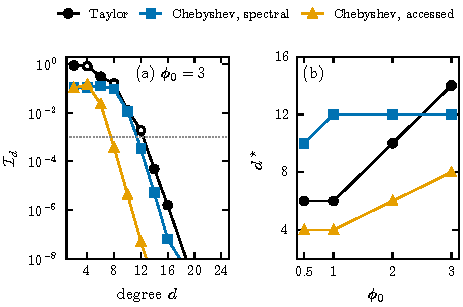
\includegraphics[width=\columnwidth]{figures/fig_sg_polynomial.pdf}
\caption{Polynomial approximation overhead for replacing the native Josephson cosine of one site (\(E_J=1\), \(\omega_b=1\), \(T=1\), \(n_{\rm cut}=64\)). (a) Maximum trajectory infidelity against the native-cosine evolution as a function of polynomial degree for \(\phi_0=3\). Open markers are cutoff-limited, with top-level population above \(10^{-5}\), and the dotted line is the criterion \(10^{-3}\). (b) Minimum degree \(d^\star\) meeting the criterion among the candidates \(2,4,\ldots,16,20,24\), as a function of the initial displacement.}
\label{fig:sg-polynomial-degree}
\end{figure}

\section{Finite representations and numerical methods}
\label{app:numerics}

All calculations use double-precision dense or sparse matrices with Python 3.13.0, NumPy 2.3.4, and SciPy 1.16.3. States from different cutoffs are compared after zero padding in the same Fock basis, and coherent initial states are projected onto each cutoff and normalized, with classical initial data taken from the first moments of the represented state.

\paragraph{Operators.}
For the Duffing oscillator the quartic polynomial is formed in a space of dimension \(N+4\) and then projected, which gives the strict sandwich \(P_N\hat H_{\rm D}P_N\), and trajectories are computed by exact diagonalization on a 401-point grid. For the lattice models we use the finite spectral convention, in which \(\hat\Pi_j^2\) and \(\cos(m\hat\phi_j)\) are matrix functions of the truncated quadratures of Eq.~\eqref{eq:sg-quadratures}, with the cosine evaluated through the eigendecomposition of the truncated \(\hat\phi_j\). Replacing this model by projected infinite-oscillator matrix elements changes the double sine-Gordon target state at local cutoff 128 by at most \(9.9\times10^{-5}\) in projective distance at the outer-step times and \(C_{12}\) by \(5.6\times10^{-9}\).

\paragraph{Integration.}
The sine-Gordon calibration of Sec.~\ref{subsec:sg-classical} uses a Strang split-operator propagator with 1024 steps over the window, a 2048-step refinement, and a 257-point observation grid. The double sine-Gordon reference applies the sparse matrix exponential at 257 times and is checked against an adaptive eighth-order Runge--Kutta integration (DOP853, relative tolerance \(2\times10^{-11}\)). Classical references use DOP853 with relative tolerance \(2\times10^{-10}\). Crossing times \(t_{\rm E}\) are interpolated linearly within the grid interval where the threshold is first exceeded.

\paragraph{Acceptance criteria and margins.}
For a compiled circuit the state error is the maximum of the projective or Bures distance from the reference, plus three empirical margins: the reference margin, given by the change of the reference between two cutoffs, the solver margin, given by the difference from an independent integration, and the padding margin, given by the change of the circuit output between two padding cutoffs with unchanged parameters. The maximum runs over the outer-step times for the double sine-Gordon step scan and over the common times \(t_j=jT/10\) for the Duffing circuits and for the double sine-Gordon comparison at \(r=10\) and 20 of Fig.~\ref{fig:dsg-subdivisions}. The state criterion requires this sum to be at most \(\sqrt{10^{-3}}\). The boundary criterion requires the population of the four highest levels of each mode to stay below \(10^{-6}\) at both padding cutoffs, monitored after every outer step and potential block and, for SNAP+D circuits, after every SNAP gate and displacement. For the double sine-Gordon lattice the observable criteria require \(\max_j|\Delta C_{12}|+u_C\le0.01\) with \(u_C\le10^{-3}\) and \(\max_j|\Delta S_2|+u_S\le0.02\) with \(u_S\le5\times10^{-3}\), where \(u\) denotes the numerical uncertainty of the observable. Duffing reference cutoffs are 64 and 80 with circuit paddings 96 and 112. The double sine-Gordon step scan uses reference and padding cutoffs 128 and 160, with the solver margin of an independent DOP853 integration at cutoff 160, and the comparison of Fig.~\ref{fig:dsg-subdivisions} uses 96 and 128.

\paragraph{Outer splitting errors.}
The splitting errors of Fig.~\ref{fig:dsg-resources}(b) use exact blocks at local cutoff 80. The correction, the retuned correction, and the potentials act as diagonal phases in the eigenbasis of the truncated \(\hat\phi_j\), and the native, kinetic, and Gaussian blocks are applied with the sparse matrix exponential. The error is the maximum projective distance from the exact target at the same cutoff over the outer-step times, for \(r=5\), 7, 10, 14, 20, 28, and 40. At \(r=10\) and 20 the values change by at most 1.4\% between local cutoffs 64 and 80, and on the same time grid they agree with the compiled circuits with second-order blocks and \(s=32\) at cutoff 128 to within 0.6\%. The sweep of Fig.~\ref{fig:dsg-resources}(c) uses local cutoff 64. At \(\kappa=2\) and \(\lambda_2=0.6\) its kinetic--potential value at \(r=20\) changes by 4.8\% at local cutoff 80, and the other values change by less than 0.4\%.

\paragraph{Three-site calculations.}
On three sites every propagation \(e^{-i\tau H}\), for the reference and for the native steps of the hybrid circuit, uses an adaptive Lanczos propagator \cite{Park1986Lanczos,Hochbruck1997Krylov} with full reorthogonalization and an error tolerance of \(10^{-11}\) per propagation, and the two qubit components are propagated separately. On two sites this propagator reproduces the state errors of the step scan at the printed precision. On three sites it agrees with the \texttt{expm\_multiply} propagator of SciPy to \(6\times10^{-14}\) over one native half step at local cutoff 96, and SciPy propagations of the target to \(T\) at local cutoffs 64 and 80 differ from the Lanczos state at cutoff 128 by \(2.8\times10^{-4}\) and \(7.0\times10^{-5}\). The solver margin is the difference from a single propagation to \(T\) with tolerance \(10^{-13}\), \(3\times10^{-8}\). At local cutoff 128 the three-site target has population below \(9\times10^{-8}\) in states with some mode above level 60 at the stored times, against \(3.8\times10^{-5}\) for the two-site target, and it changes by \(1.7\times10^{-6}\) between local cutoffs 128 and 160.

\paragraph{Compiler.}
The SNAP+D parameters minimize \(J=\|e^{-i\gamma}Y_{\rm comp}-Y_{\rm target}\|_F^2/N_{\rm train}+\nu\,{\rm mean}_\ell|\alpha_\ell|^2\) with a single phase \(\gamma\) shared by all \(N_{\rm train}\) training columns and \(\nu=10^{-8}\), where the columns of \(Y_{\rm comp}\) and \(Y_{\rm target}\) are the compiled and exact block outputs. Gradients use the Fr\'echet derivative of the actual finite matrix exponential. We use SciPy's SLSQP with \texttt{ftol} \(10^{-12}\), phase bounds \([-\pi,\pi]\), and bounds \([-1.5,1.5]\) on the real and imaginary parts of each displacement. For the Duffing circuit of Sec.~\ref{subsec:df-compile}, three starts ran to the limit of 5000 iterations in about 210\,s each on one core, and the start with the lowest training objective, \(8.0\times10^{-6}\), was selected before any evaluation. Each start sets the first SNAP layer to the phases of the diagonal of the target block and places pairs of opposite displacements \(D(\alpha)D(-\alpha)=I\) with \(|\alpha|\) uniform in \([0.3,0.8]\) and random phase, so the initial circuit is number diagonal while the displacement gradients do not vanish. The twelve random evaluation states have amplitudes uniform in \([1,2.25]\) and phases uniform in \([0,2\pi)\), drawn with a fixed seed before training.

\section{Duffing compiler: training coverage}
\label{app:duffing-training}

Circuits trained on the trajectories of three real coherent amplitudes, 1, 1.5, and 2.25, for \(r\in\{10,20\}\) and \(L\in\{4,8,12\}\), with three starts each and 1200 iterations, reproduce the two real benchmark states with amplitude errors of at most 0.031. On the ten development inputs of Sec.~\ref{subsec:df-compile}, however, the six selected circuits reach worst distances between 0.85 and 1.38, always at the input \(\ket{2i}\) (Fig.~\ref{fig:df-training}). On the eight development inputs outside the training arc, the compiled circuit is farther from the target than Kerr evolution with the exact Gaussian correction in 45 of 48 cases. Running the \(L=8\) fit to solver convergence, at 2891 iterations, lowers its training objective from \(2.1\times10^{-5}\) to \(4.1\times10^{-6}\), but the circuit then passes only 5 of the 22 inputs of Sec.~\ref{subsec:df-compile}. Over \(T=1\) the harmonic rotation turns a coherent state by about one radian, so the states entering the quartic block from real initial amplitudes cover only an arc of phase space, and \(\hat V_4\), which is not rotation invariant, acts differently elsewhere. The circuit of Sec.~\ref{subsec:df-compile} is trained on eight initial phases with \(L=12\) layers. Its training also uses paired-displacement initialization and up to 5000 iterations, so the comparison does not isolate the contribution of phase coverage.

\begin{figure}[t]
\centering
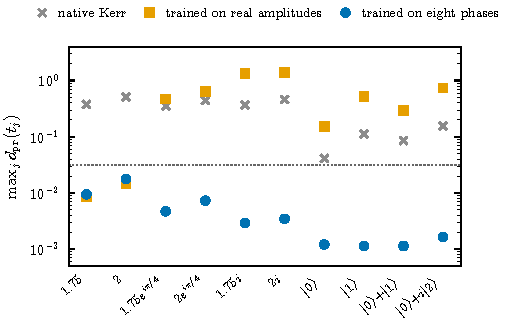
\includegraphics[width=\columnwidth]{figures/fig_duffing_training.pdf}
\caption{Maximum projective distance on the ten development inputs for native Kerr evolution and for two compiled Duffing circuits with \(r=10\) and \(L=12\), one trained on real coherent amplitudes and one trained on eight initial phases. The dotted line is \(\sqrt{10^{-3}}\).}
\label{fig:df-training}
\end{figure}

\section{SNAP-plus-displacement correction of the double sine-Gordon lattice}
\label{app:dsg-snap}

The local SNAP+D correction was fitted to the action of \(e^{-ih\lambda_2(1-\cos2\hat\phi)}\) on the first 16 Fock states at local cutoff 48 with \(d=24\) SNAP levels, and the same circuit acted on both sites between native half steps. Table~\ref{tab:dsg-snap} lists four searches, all evaluated with the full two-site circuit at cutoffs 96/128. The larger fits meet both observable criteria but not the state criterion, and a longer optimization of the larger fit lowers its training loss while its state error rises from 0.057 to 0.059.

The failure of the zero-displacement starts has a symmetry origin. The local target commutes with the parity \(\mathcal P=(-1)^{\hat N}\), and the Fock-state training inputs are parity eigenstates, so the matrices \(X\) of training inputs and \(Y\) of target outputs satisfy \(\mathcal PX=X\Theta\) and \(\mathcal PY=Y\Theta\) with a diagonal sign matrix \(\Theta\). Since \(\mathcal PD(\alpha)\mathcal P=D(-\alpha)\) and SNAP gates commute with \(\mathcal P\), the objective is invariant under reversal of all displacements, and its displacement gradient vanishes at zero displacement for every choice of SNAP phases. Zero-displacement starts therefore remain at number-diagonal circuits, which cannot reproduce the correction (Proposition~\ref{prop:diagonal}). Starts built from opposite displacement pairs, as in Appendix~\ref{app:numerics}, avoid the stationary point but do not reach the state criterion within the tested iteration limits. The reference state of the target also has population \(4.2\times10^{-3}\) outside the first 16 levels of either mode at the final time, so the 16 training columns do not span the states on which the correction acts.

\begin{table}[t]
\caption{SNAP+D searches for the double sine-Gordon correction: zero-displacement starts, starts with paired opposite displacements, a larger training space, and a longer optimization of the larger fit. Dimensions are (local training cutoff, SNAP levels, training columns). The state error \(e_B\) includes numerical margins and spans the selected circuits of each search. No circuit meets \(\sqrt{10^{-3}}\approx0.032\).}
\label{tab:dsg-snap}
\begin{ruledtabular}
\begin{tabular}{lccccc}
Search & Dimensions & \(r\) & \(L\) & Starts & \(e_B\) \\
\hline
Zero displ. & (48,24,16) & 10, 20 & 2, 4, 6 & 18 & 0.103--0.144 \\
Paired & (48,24,16) & 10, 20 & 2, 4, 6 & 18 & 0.080--0.179 \\
Larger & (96,48,32) & 10 & 12 & 3 & 0.057 \\
Longer & (96,48,32) & 10 & 12 & 1 & 0.059 \\
\end{tabular}
\end{ruledtabular}
\end{table}

\section{Trigonometric gate construction and primitive counts}
\label{app:trig}

Operator products act from the right. For site \(j\) and harmonic \(m\), let \(A=m\hat\phi_j\) and, with a qubit that starts in \(\ket0\), define \(\mathcal U=e^{iA\otimes X/2}\), \(\Sigma_+=\mathcal UZ\mathcal U^\dagger=\cos A\otimes Z+\sin A\otimes Y\), and \(\Sigma_-=\mathcal U^\dagger Z\mathcal U=\cos A\otimes Z-\sin A\otimes Y\). Then \(\Sigma_++\Sigma_-=2\cos A\otimes Z\), and the exact exponentials \(E_\pm(v)=e^{iv\Sigma_\pm}\) combine into the first- and second-order blocks
\begin{align}
Q^{(1,s)}(u)&=e^{-iu}\big[E_+(u/2s)E_-(u/2s)\big]^s,\nonumber\\
Q^{(2,s)}(u)&=e^{-iu}\big[E_+(u/4s)E_-(u/2s)E_+(u/4s)\big]^s,
\end{align}
which approximate \(e^{-iu(1-\cos A)}\) on the qubit state \(\ket0\) for \(u=hc\) and a potential coefficient \(c\) \cite{Rainaldi2026TrigonometricCV}. These identities hold for any finite Hermitian \(A\). With \(R_y(\theta)=e^{-i\theta Y/2}\), \(R_z(\theta)=e^{-i\theta Z/2}\), and the qubit-controlled displacement \({\rm CD}_Z(\alpha)=\exp[(\alpha\hat a^\dagger-\alpha^*\hat a)\otimes Z]\) \cite{Eickbusch2022ECD}, the factor \(D_A=e^{iA\otimes Z/2}={\rm CD}_Z\bigl(im/(2\sqrt{2\omega_b})\bigr)\) is a single controlled displacement. The rotation \(B=R_y(\pi/2)R_z(\pi/2)\) maps \(Z\) to \(X\) and \(Y\) to \(Z\) under conjugation, so \(\mathcal U=\mathcal BD_A\mathcal B^\dagger\) with \(\mathcal B=I\otimes B\), and
\begin{align}
E_+(v)&=\mathcal B\,D_A\,R_y(-2v)\,D_A^\dagger\,\mathcal B^\dagger,\nonumber\\
E_-(v)&=\mathcal B\,D_A^\dagger\,R_y(-2v)\,D_A\,\mathcal B^\dagger .
\end{align}
The products \(\mathcal B^\dagger\mathcal B\) between consecutive factors cancel, and \(\mathcal B\) commutes with the native and Gaussian blocks, which act on the system alone. A circuit therefore applies \(\mathcal B^\dagger\) once at the start and \(\mathcal B\) once at the end, an unmerged \(E_\pm\) uses two controlled displacements and one \(R_y\), and a harmonic block uses \(4s\) controlled displacements and \(2s\) \(R_y\) rotations at first order and \(6s\) and \(3s\) at second order before merging. On a finite test space the merged pulse sequences reproduce the exact blocks to \(3\times10^{-15}\), and whole circuits on two and three sites, with a random system unitary in place of the native and Gaussian blocks between the outer steps, reproduce the original construction to \(2\times10^{-14}\). The simulations apply the exact factors \(E_\pm\), which give the same circuit unitary, so the qubit populations quoted in Sec.~\ref{sec:dsg} refer to the frame of these factors, which differs from that of the compiled pulses by \(\mathcal B\) between the first and the last pulse. System observables and oscillator populations do not depend on this frame. The potential circuit applies site 1 with harmonics \(m=1,2\) and then site 2, skipping zero coefficients, and reuses one qubit coherently throughout, so the blocks of different sites run serially. The same qubit is traced out only at the end. Adjacent rotations about the same axis and adjacent controlled displacements are merged exactly. The bond step of the kinetic--potential circuit consists of two local \(\hat\phi_j^2\) phases and one \(e^{ih\kappa\hat\phi_1\hat\phi_2}\) gate, and each kinetic half step of two local \(\hat\Pi_j^2\) phases, so its Gaussian gates number \(5r+2\). Counts in Table~\ref{tab:dsg-resources} include all merges. With \(s=1\) the hybrid circuit uses \(10r+4\) primitives with first-order and \(14r+4\) with second-order blocks, and the trigonometric part of a programmable circuit uses \(18r+4\) and \(26r+4\), or \(22r+4\) with a second-order block for the Josephson harmonic and a first-order block for the \(\lambda_2\) harmonic, where the constant 4 counts the rotations of \(\mathcal B^\dagger\) and \(\mathcal B\). Counting the final \(\mathcal B\), which only returns the qubit to its computational frame before the qubit is traced out, lowers every saving slightly. The Gaussian-block circuit writes each exact Gaussian step as \(e^{-i\tau(H_{\rm kin}+H_{\rm bond})}=\mathcal G_\phi\mathcal G_\Pi\mathcal G_\phi\), with \(\mathcal G_\phi=\exp[-i\tfrac a2(\hat\phi_1-\hat\phi_2)^2]\) and \(\mathcal G_\Pi=\exp\{-i[(\tfrac\tau4+\tfrac b2)(\hat\Pi_1^2+\hat\Pi_2^2)+(\tfrac\tau2-b)\hat\Pi_1\hat\Pi_2]\}\), where \(\omega=\sqrt{2\kappa}\), \(b=\sin(\omega\tau)/(2\omega)\), and \(a=\tfrac\omega2\tan(\omega\tau/2)\). For canonical operators this is the exact shear decomposition of the oscillator formed by the antisymmetric mode, with the free symmetric mode absorbed into \(\mathcal G_\Pi\). The truncated quadratures do not obey the canonical commutation relation, so at finite cutoff the product differs from the truncated block \(e^{-i\tau(H_{\rm kin}+H_{\rm bond})}\). On the 14 states that enter the Gaussian factors of the cheapest circuit at \(\lambda_2=0.3\), the difference has norm at most \(6.7\times10^{-4}\) at local cutoff 128 and \(2.6\times10^{-4}\) at 160, and for the cheapest circuits at \(\lambda_2=0.1\) and 0.6 it is at most \(5.9\times10^{-4}\) at cutoff 128. The circuits apply the factors, so the state errors of Table~\ref{tab:dsg-resources} include this difference. Each factor consists of two local quadratic phases and one two-mode gate, the momentum gate being the Fourier conjugate of the bond gate. Adjacent \(\mathcal G_\phi\) factors commute through the potential block and merge, so the circuit has \(6r+9\) Gaussian primitives. On \(N\) sites the same construction uses the normal modes of the bond Laplacian, and each factor has \(N\) local terms and up to \(N(N-1)/2\) two-mode terms. On three sites the Gaussian-block circuit therefore has \(12r+18\) Gaussian primitives, the kinetic--potential circuit \(8r+3\), and the trigonometric parts use \(15r+4\) primitives for the first-order hybrid circuit and \(33r+4\) for the programmable circuits with mixed block orders. At \(\lambda_2=0\) the correction vanishes, and the exact symmetric split reproduces the target to \(3\times10^{-14}\), which checks the splitting code.

Figure~\ref{fig:dsg-subdivisions} shows the comparison restricted to \(r=10\) and 20 at cutoffs 96/128, with \(s\) from 1 to 32. Larger \(s\) halves the state error of first-order kinetic--potential circuits at \(r=20\), but second-order blocks with \(s=1\) are cheaper and more accurate, and larger \(s\) never lowers the cheapest passing count of any route. At padding cutoff 96 the target state itself has boundary population \(7.7\times10^{-7}\), and the \(r=20\) kinetic--potential circuits and the 104-primitive hybrid circuit exceed \(10^{-6}\) there by up to 8\%. At cutoffs 128/160 every circuit of the step scan at \(\lambda_2=0.1\) and 0.3 meets the boundary criterion. At \(\lambda_2=0.6\) sixteen of the evaluated circuits exceed it at padding 128, among them the three Gaussian-block circuits with mixed block orders and \(r=10\) to 12, which meet the state and observable criteria there and every criterion at cutoffs 160/192 (Sec.~\ref{sec:dsg}).

\begin{figure}[t]
\centering
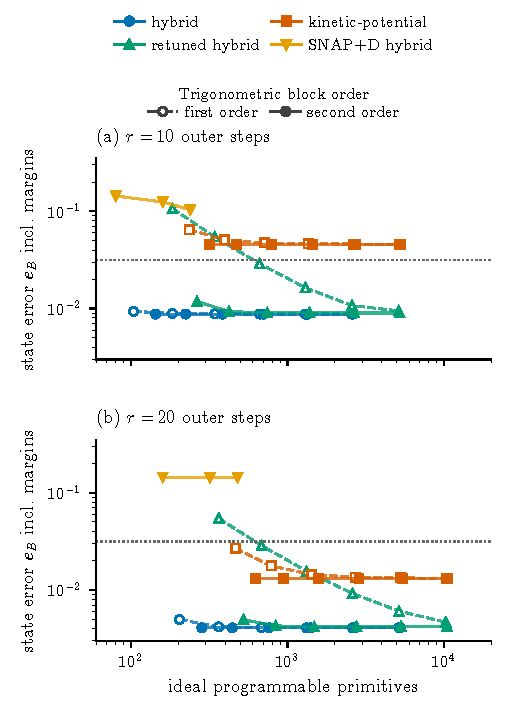
\includegraphics[width=\columnwidth]{figures/fig_dsg_subdivisions.pdf}
\caption{Double sine-Gordon circuits restricted to \(r=10\) (circles) and \(r=20\) (squares) outer steps, at reference and padding cutoffs 96/128. State error including numerical margins against the number of ideal programmable primitives, with open symbols for first-order and filled symbols for second-order blocks and lines connecting \(s=1,2,4,8,16,32\) internal subdivisions. SNAP+D hybrid circuits (triangles) use \(L=2,4,6\) layers. Points below the dotted line \(\sqrt{10^{-3}}\) can fail the boundary criterion at padding cutoff 96.}
\label{fig:dsg-subdivisions}
\end{figure}

\section{Double sine-Gordon reference convergence and acceptance checks}
\label{app:dsg-convergence}

The two-site double sine-Gordon target requires larger local cutoffs for the state than for the observables. Table~\ref{tab:dsg-convergence} lists the maximum changes between adjacent cutoffs. The change between cutoffs 64 and 96 is \(6.9\times10^{-3}\), and the state resolution requirement \(\sqrt{10^{-3}}/10\) is met from the pair 96/128 on, while \(C_{12}\) and \(S_2\) are resolved already at small cutoffs. An independent DOP853 integration at cutoff 128 differs from the sparse-exponential trajectory by at most \(2.7\times10^{-9}\). For the second preparation of Sec.~\ref{sec:dsg}, the reference changes by \(2.5\times10^{-4}\) between cutoffs 128 and 160.

\begin{table}[t]
\caption{Maximum change of the double sine-Gordon target between adjacent local cutoffs, for the state at the times \(t_j=jT/10\) and for \(C_{12}\) and \(S_2\) on the 257-point observation grid.}
\label{tab:dsg-convergence}
\begin{ruledtabular}
\begin{tabular}{lccc}
Cutoffs & State distance & \(|\Delta C_{12}|\) & \(|\Delta S_2|\) \\
\hline
32/48 & \(4.3\times10^{-2}\) & \(8.1\times10^{-4}\) & \(3.1\times10^{-6}\) \\
48/64 & \(1.7\times10^{-2}\) & \(9.0\times10^{-5}\) & \(4.3\times10^{-8}\) \\
64/96 & \(6.9\times10^{-3}\) & \(2.6\times10^{-5}\) & \(6.8\times10^{-11}\) \\
96/128 & \(1.3\times10^{-3}\) & \(1.3\times10^{-6}\) & \(1.4\times10^{-11}\) \\
128/160 & \(2.3\times10^{-4}\) & \(3.6\times10^{-8}\) & \(1.3\times10^{-13}\) \\
\end{tabular}
\end{ruledtabular}
\end{table}

\paragraph{Common readout times.}
Because each circuit is checked at its own outer-step times \(jT/r\), we repeated the test for the cheapest circuits and for the circuits with one outer step fewer at the common times \(t_k=kT/20\), \(k=1,\ldots,20\), which are finer than the outer-step grid of every circuit in Table~\ref{tab:dsg-resources}. Each time \(t_k\) is reached by its own circuit of \(n_k=\lceil t_k/h\rceil\) equal outer steps of length \(t_k/n_k\le h\), so no partial step is needed and no readout circuit has more primitives than the circuit to \(T\). The margins, observable errors, and boundary populations are evaluated with the same rule at these times. At each of the three values of \(\lambda_2\) the cheapest circuits of Table~\ref{tab:dsg-resources} pass again, the Gaussian-block circuit at \(\lambda_2=0.6\) with cutoffs 160/192 as in the table, and the circuits with one outer step fewer fail, so the cheapest counts are unchanged. At \(\lambda_2=0.3\) the state errors of the three cheapest circuits are 0.0271, 0.0286, and 0.0288 at the common times, against 0.0271, 0.0298, and 0.0307 on their own grids, and every other circuit with fewer primitives fails as well, most of them already at \(t=T\), which both grids contain. These checks sample the trajectory at finitely many times and do not bound the error between them.

\paragraph{Tighter thresholds.}
Table~\ref{tab:dsg-thresholds} lists the cheapest circuit of each route when the state criterion is tightened from \(\sqrt{10^{-3}}\) to \(\sqrt{\mathcal I_\star}\), with the reference margin required to stay below a tenth of that value and the boundary, \(C_{12}\), and \(S_2\) criteria unchanged. Each entry is the cheapest passing circuit among those evaluated, and for each entry the circuit with the same block orders and one outer step fewer was evaluated and fails. The hybrid circuit is the cheapest route at every threshold, and its saving relative to the Gaussian-block circuit ranges from 2.6 to 4.6.

\begin{table}[t]
\caption{Cheapest two-site double sine-Gordon circuits of each route at infidelity threshold \(\mathcal I_\star\) (cutoffs 128/160, \(E_J=\kappa=1\), \(s=1\)), given as the number of ideal programmable primitives with the number \(r\) of outer steps in parentheses. The last two columns are the ratios of the Gaussian-block (GB) and kinetic--potential (KP) counts to the hybrid count. Entries marked \(\ast\) exceed the boundary limit only at padding 128 and are evaluated at cutoffs 160/192.}
\label{tab:dsg-thresholds}
\begin{ruledtabular}
\begin{tabular}{llccccc}
\(\lambda_2\) & \(\mathcal I_\star\) & Hybrid & GB & KP & GB & KP \\
\hline
0.1 & \(10^{-3}\) & 54 (5) & 181 (6) & 330 (12) & 3.4 & 6.1 \\
  & \(5\times10^{-4}\) & 54 (5) & 209 (7) & 384 (14) & 3.9 & 7.1 \\
  & \(2.5\times10^{-4}\) & 54 (5) & 237 (8) & 465 (17) & 4.4 & 8.6 \\
  & \(10^{-4}\) & 64 (6) & 293 (10) & 573 (21) & 4.6 & 9.0 \\
0.3 & \(10^{-3}\) & 64 (6) & 209 (7) & 330 (12) & 3.3 & 5.2 \\
  & \(5\times10^{-4}\) & 74 (7) & 237 (8) & 411 (15) & 3.2 & 5.6 \\
  & \(2.5\times10^{-4}\) & 84 (8) & 293 (10) & 465 (17) & 3.5 & 5.5 \\
  & \(10^{-4}\) & 94 (9) & 349 (12) & 600 (22) & 3.7 & 6.4 \\
0.6 & \(10^{-3}\) & 94 (9) & 293 (10)\(^\ast\) & 357 (13) & 3.1 & 3.8 \\
  & \(5\times10^{-4}\) & 104 (10) & 321 (11)\(^\ast\) & 411 (15) & 3.1 & 4.0 \\
  & \(2.5\times10^{-4}\) & 134 (13) & 349 (12)\(^\ast\) & 492 (18) & 2.6 & 3.7 \\
  & \(10^{-4}\) & 172 (12) & 461 (16) & 627 (23) & 2.7 & 3.6 \\
\end{tabular}
\end{ruledtabular}
\end{table}

\section{Formal verification}
\label{app:lean}

Several statements of this work are formalized in Lean~4 (version 4.33.0-rc1, with Mathlib at revision 79d0395), and the formal proofs contain no unproved steps. The formalized statements include the exact split of Eq.~\eqref{eq:df-split} for the strict-cutoff Duffing Hamiltonian and its Hermiticity, the phase-aligned bounds of Eqs.~\eqref{eq:df-duhamel} and \eqref{eq:df-bound}, the squeezing identity of Eq.~\eqref{eq:df-squeezing}, the number-diagonal ceiling of Proposition~\ref{prop:diagonal}, the Gaussian expectation of Eq.~\eqref{eq:debye-waller}, the Kerr first-moment formula and collapse time of Sec.~\ref{subsec:encoding}, the Hermiticity of the finite sine-Gordon Hamiltonian, and the telescoping inequality underlying Eq.~\eqref{eq:action-sum} as an abstract norm bound. Theorem~\ref{thm:native-residual}, Eq.~\eqref{eq:classical-transfer}, and the physical gate identities of Appendix~\ref{app:trig} are proved on paper.


\end{document}
